% Full instructions available at:
% https://github.com/elauksap/focus-beamertheme

\documentclass[aspectratio=169]{beamer}
\usetheme{focus}
\usepackage{colortbl}
\usepackage{hyperref}
\usepackage{xcolor}
\usepackage[export]{adjustbox}
\usepackage{tikz}
\usepackage{amsmath} % for \boxed and \smash[b] macros
\usepackage{booktabs}% for \midrule and \cmidrule macros
\newcommand\headercell[1]{%
   \smash[b]{\begin{tabular}[t]{@{}c@{}} #1 \end{tabular}}}
\usepackage{float}

\usetikzlibrary{positioning,shapes}
\newcommand{\Lumi}{ \mathcal{L}}

\newcommand*{\myfont}{\fontfamily{lmtt}\selectfont}


\title{\Large{Towards a Deeply Virtual Neutral Pion Production\newline Cross Section Measurement at CLAS12}}
\subtitle{Fall 2022 DNP Meeting}
\institute{Massachusetts Institute of Technology \\ CLAS12 Collaboration}
\usepackage{caption}
\captionsetup[figure]{labelformat=empty}
\titlegraphic{
\includegraphics[scale=.15]{Pics/Intro/mit-clas12-combined.PNG}}
\author{R. Johnston\texorpdfstring{\\}{,}}
%\date{\today}
\date{Friday, October 28, 2022}


\usepackage{array}
\newcolumntype{P}[1]{>{\centering\arraybackslash}p{#1}}

\definecolor{mygreen}{RGB}{14, 176, 9}
\definecolor{myyellow}{RGB}{204, 204, 10}
\definecolor{mypink}{RGB}{255, 51, 255}
\definecolor{mypurp}{RGB}{153, 21, 255}


\definecolor{lightred}{RGB}{255, 132, 145}
\definecolor{darkred}{RGB}{201, 49, 2}
\definecolor{lightorange}{RGB}{255, 200, 84}
\definecolor{darkorange}{RGB}{225, 150, 0}

\definecolor{lightgreen}{RGB}{85, 255, 91}
\definecolor{darkgreen}{RGB}{0, 170, 6}
\definecolor{lightblue}{RGB}{88, 200, 255}
\definecolor{darkblue}{RGB}{0, 81, 203}


\definecolor{sigmaT}{RGB}{0, 0, 0}
\definecolor{sigmaL}{RGB}{0, 0, 0}
\definecolor{sigmaLT}{RGB}{252, 3, 3}
\definecolor{sigmaTT}{RGB}{3, 32, 252}




% Chiral Even GPDs
\newcommand{\GPDH}{\textcolor{lightred}{${H}$}}
\newcommand{\GPDHEQ}{\textcolor{lightred}{{H}}}

\newcommand{\GPDE}{\textcolor{lightgreen}{${E}$}}
\newcommand{\GPDEEQ}{\textcolor{lightgreen}{{E}}}

\newcommand{\GPDHtilde}{\textcolor{lightorange}{$\tilde{H}$}}
\newcommand{\GPDHtildeEQ}{\textcolor{lightorange}{\tilde{H}}}

\newcommand{\GPDEtilde}{\textcolor{lightblue}{$\tilde{E}$}}
\newcommand{\GPDEtildeEQ}{\textcolor{lightblue}{\tilde{E}}}



%Chiral Odd GPDs

\newcommand{\GPDHT}{\textcolor{darkred}{$H_T$}}
\newcommand{\GPDHTEQ}{\textcolor{darkred}{H_T}}

\newcommand{\GPDET}{\textcolor{darkgreen}{$E_T$}}
\newcommand{\GPDETEQ}{\textcolor{darkgreen}{E_T}}

\newcommand{\GPDHTtilde}{\textcolor{darkorange}{$\tilde{H}_T$}}
\newcommand{\GPDHTtildeEQ}{\textcolor{darkorange}{\tilde{H}_T}}


\newcommand{\GPDETtilde}{\textcolor{darkblue}{$\tilde{E}_T$}}
\newcommand{\GPDETtildeEQ}{\textcolor{darkblue}{\tilde{E}_T}}


\newcommand{\GPDETbar}{\textcolor{mypurp}{$\bar{E}_T$}}
\newcommand{\GPDETbarEQ}{\textcolor{mypurp}{\bar{E}_T}}


    
    


\begin{document}


%\begin{frame}
%    \maketitle
%\end{frame}


\begin{frame}{Process Background}

    %\vspace{-.5cm}
         \begin{columns}[t, onlytextwidth]
         
          \column{0.35\textwidth}
            \centering Deeply Virtual $\pi^0$ Production\\
            \centering(\textcolor{alert}{DV$\pi^o$P})
            \begin{center}
                
                $e+p \rightarrow$ \\
                $e'+p' + \pi^0 \rightarrow$\\
                $e' + p' + \gamma_1 + \gamma_2$ 
            \end{center}
            
            
            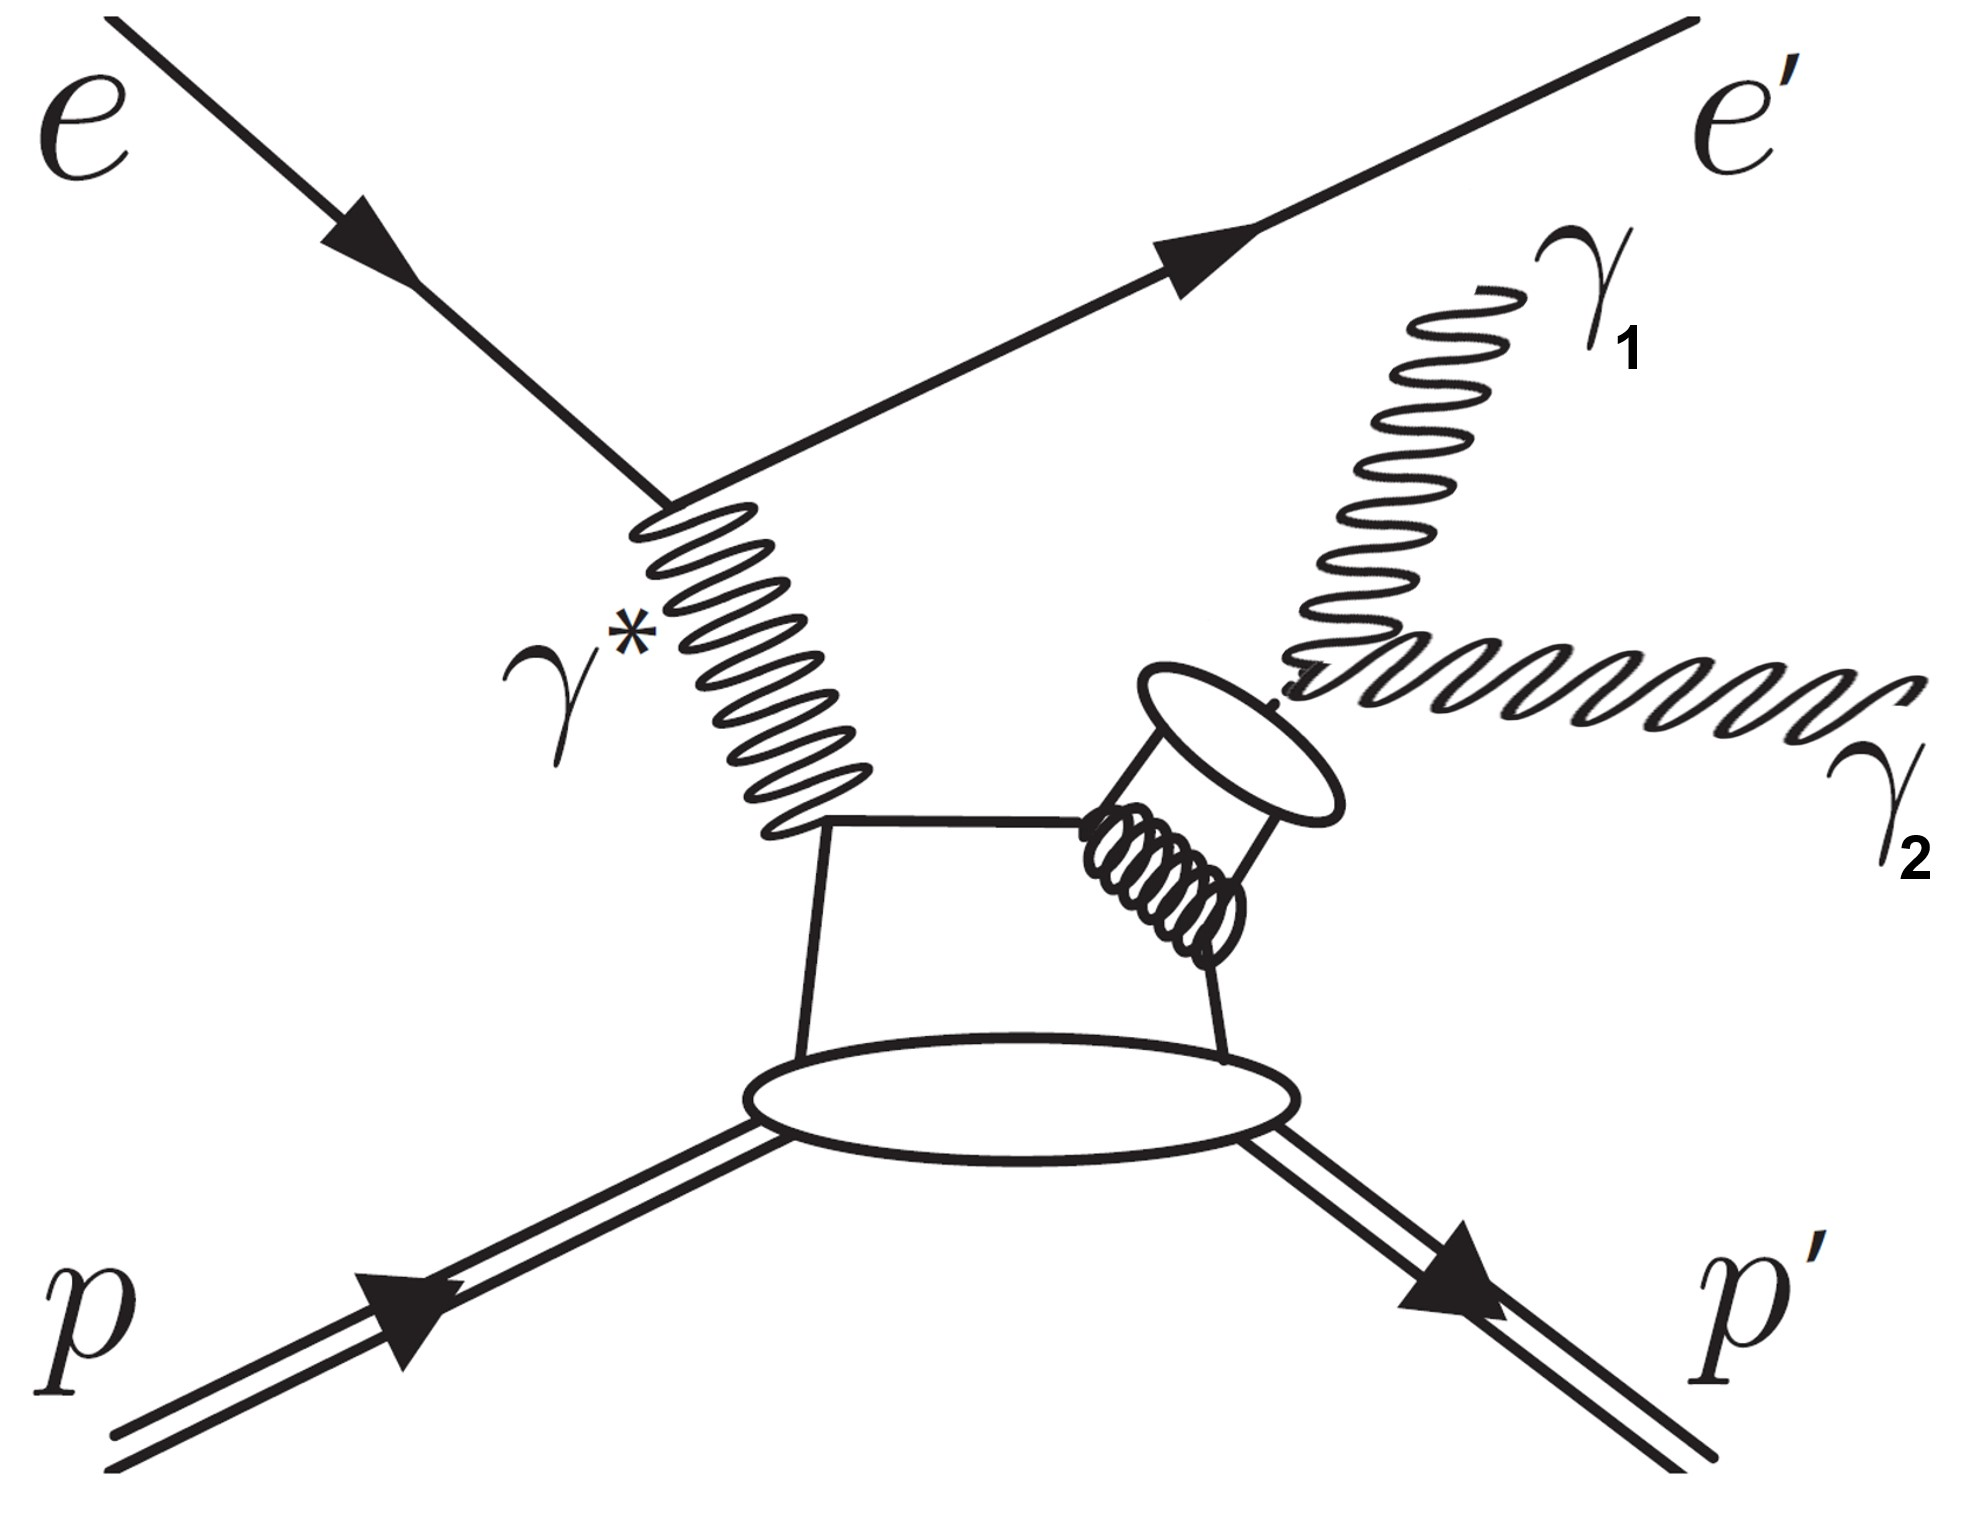
\includegraphics[trim={0 0 0 0cm} ,clip,width=.95\textwidth]{DNP/dvPiP_Feynman_diagram_2.jpg}
            
            
            
            \column{0.65\textwidth}
                \begin{itemize}
                    \setlength\itemsep{1em}
                    \item 4-fold differential cross section $\frac{d\sigma}{d\textcolor{alert}{Q^2}d\textcolor{alert}{x_B}d\textcolor{alert}{t}d\textcolor{alert}{\phi}}$ expressed in terms of:
                        \begin{itemize}
                        \setlength\itemsep{0.5em}
                            \item Virtual photon 4-momentum:  \textcolor{alert}{$Q^2$} $\equiv$  $-(p_e-p_{e'})^2$
                            \item Bjorken x: \textcolor{alert}{$x_B$} $\equiv$ $\frac{Q^2}{2p_p\cdot(p_{e}-p_{e'})}$
                            \item Momentum transfer: \textcolor{alert}{-t} $\equiv$ $-(p_{p'}-p_p)^2$
                            \item Angle between lepton \& hadron planes: \textbf{\textcolor{alert}{$\phi$}} = 
                            
                             \begin{columns}[t, onlytextwidth]
         
          \column{0.6\textwidth}
             \begin{center}
                            
                            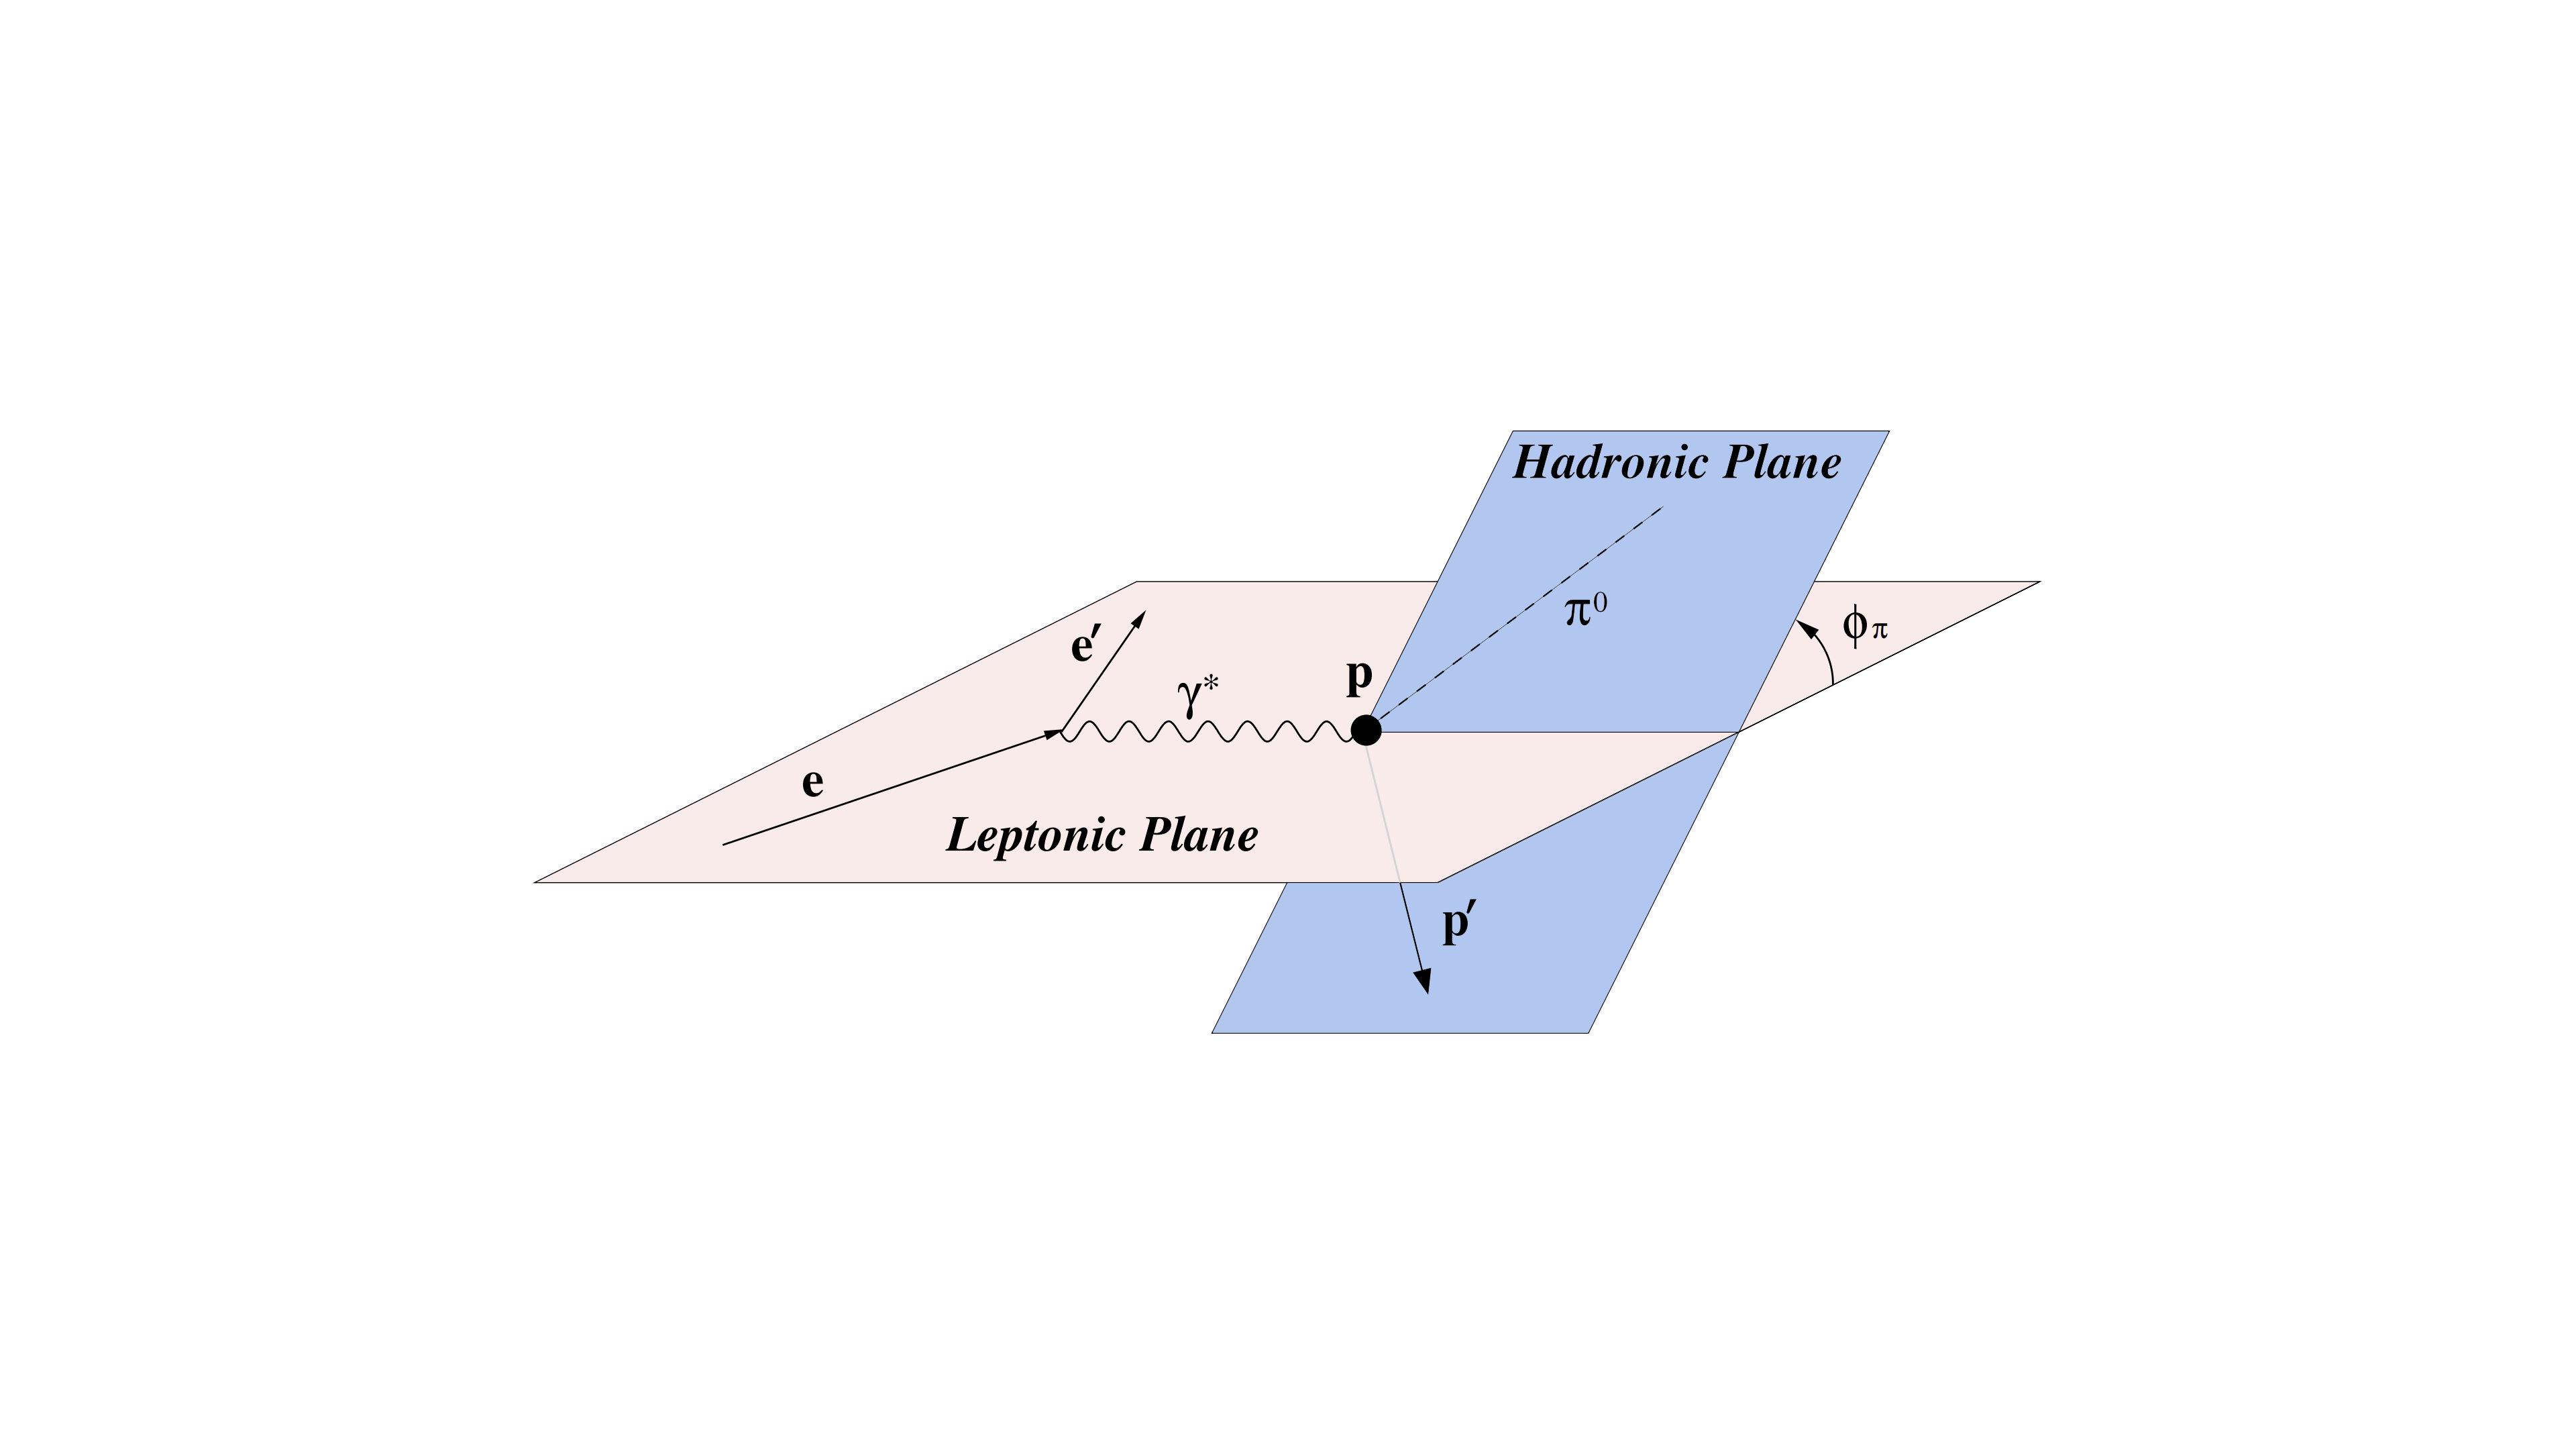
\includegraphics[trim={10cm 8cm 10cm 8cm} ,clip,width=.96546725995\textwidth]{DNP/lept_had_planes.png}
                            \end{center}
            \column{0.4\textwidth}
            \footnotesize{$\cos^{-1} \left( \frac{ \left(p_{e} \times p_{e'} \right) \cdot \left( p_{p'} \times p_{\gamma^*} \right) }{ \lVert p_{e} \times p_{e'} \rVert \: \lVert p_{p'} \times p_{\gamma^*} \rVert} \right)$}
          
          \vspace{1.5cm}
          {\myfont{\tiny     \textcolor{white}{lllllll} Images from S. Lee, A. Kim   }}
         \end{columns}
                            
                        \end{itemize}
                                            
                    \item In DIS regime: W$>2$GeV, $Q^2$> 1GeV$^2$
                \end{itemize}
                
     
                               
        \end{columns}
\end{frame}    




\begin{frame}{Physics Motivation: $DV\pi^0P$ and GPDs}



    \vspace{-.01cm}
   
    The cross section for DV$\pi^0$P has theoretically linked to Generalized Parton Distributions (GPDs), which describe the 3D structure of the nucleon:\\
    \vspace{0.1cm}
 \scalebox{0.735}{%
    $
         \frac{d^4\sigma_{\gamma^*p \rightarrow p'\pi^0}}{dQ^2dx_Bdtd\phi_{\pi}} =
         \Gamma (Q^2, x_B, E)
         \frac{1}{2\pi}
         \left\{ \left(  \textcolor{sigmaT}{\frac{d\sigma_T}{dt}}+\epsilon  \textcolor{sigmaL}{\frac{d\sigma_L}{dt}} \right)+
         \epsilon cos(2\phi)  \textcolor{sigmaTT}{\frac{d\sigma_{TT}}{dt}} + 
         \sqrt{2\epsilon(1+\epsilon)} cos(\phi)  \textcolor{sigmaLT}{\frac{d\sigma_{LT}}{dt}} \right\}
         \quad | \quad
         \Gamma (Q^2, x_B, E) = \frac{\alpha}{8\pi} \frac{Q^2}{m^2_pE^2}\frac{1-x_B}{x_B^3}\frac{1}{1-\epsilon}
    $
    }
    %\vspace{0.05cm}

    \begin{columns}
            \column{0.5\textwidth}
    

    \begin{center}
         The structure functions can be expressed in terms of GPDs:
    \end{center}
   
    %\vspace{0.05cm}
   
    \scalebox{0.80}{%   
    $      \textcolor{sigmaL}{\frac{d\sigma_{L}}{dt}} = 
    \frac{4\pi\alpha}{kQ^2}\left\{ \left( 1 - \xi^2 \right) 
    \lvert \langle \GPDHtildeEQ \rangle \rvert ^2 
    -2\xi^2 \Re \left[  \langle \GPDHtildeEQ \rangle ^* \langle \GPDEtildeEQ \rangle    \right] - \frac{t'}{4m^2}\xi^2
    \lvert \langle \GPDEtildeEQ \rangle \rvert ^2  \right\}$
    }\\
    
    \scalebox{0.80}{%   
    $      \textcolor{sigmaT}{\frac{d\sigma_{T}}{dt}} = 
    \frac{2\pi\alpha \mu_{\pi}^2}{kQ^4}
    \left\{ \left( 1 - \xi^2 \right) 
    \lvert \langle \GPDHTEQ \rangle \rvert ^2
    - \frac{t'}{8m^2}
    \lvert \langle \GPDETbarEQ \rangle \rvert ^2  \right\}$
    }\\
    
    \scalebox{0.80}{%   
    $     \textcolor{sigmaLT}{\frac{d\sigma_{LT}}{dt}} = 
    \frac{4\pi\alpha \mu_{\pi}}{\sqrt{2}kQ^3}
    \xi\sqrt{1-\xi^2}
    \frac{\sqrt{-t'}}{2m}
    \Re \left\{ 
     \langle \GPDHTEQ \rangle ^*
    \langle \GPDEtildeEQ \rangle   
    \right\}$
    }\\
    
    \scalebox{0.80}{%   
    $      \textcolor{sigmaTT}{\frac{d\sigma_{TT}}{dt}} = 
    \frac{4\pi\alpha \mu_{\pi}^2}{kQ^4}
    \frac{-t'}{16m^2}
    \langle \GPDETbarEQ \rangle^2   
    $
    }\\
    

   
 
    
    \column{0.5\textwidth}
    
    \centering 
    %\vspace{0.3cm}
    GPD Classification:\\\tiny{\textcolor{white}{lll}}\\
         %\vspace{0.1cm}
         \footnotesize
    \scalebox{0.95}{%  
    \begin{table}[H]
        \centering
        \begin{tabular}{@{} *{4}{c} @{}}
                \headercell{Nucleon \\ Polarization} & \multicolumn{3}{c@{}}{Quark Polarization}\\
                \cmidrule(l){2-4}
                & U & \textcolor{white}{lllll}L & T    \\ 
                \midrule
                  U  & \GPDH &                                   &  \GPDETbar \\
                  L  &                    &  \textcolor{white}{llll}\GPDHtilde &                                   \\
                  T  & \GPDE &                                   &  \GPDHT,\GPDHTtilde \\
            \end{tabular}\\
            
    \end{table}
    }
            
        \vspace{0.1cm}
        \footnotesize{\GPDETbar = 2*\GPDHTtilde+\GPDET\\}
    
    \end{columns}
    \vspace{0.2cm}
    
     \begin{columns}
            \column{0.15\textwidth}
            \column{0.7\textwidth}
   \centering
   In contrast to DVCS, DV$\pi^0$P allows access to chiral-odd GPDs, making it a distinct and valuable probe
   
             \column{0.15\textwidth}
   \end{columns}
   
   \vspace{0.1cm}
   \begin{columns}
            \column{0.6\textwidth}
            \column{0.4\textwidth}

   \end{columns}
               

\end{frame}


    
    




    
\begin{frame}{\textbf{Analysis Goal}: Extract DV$\pi^o$P Cross Section}
    Extracting the cross section for the process will extend the CLAS6 work to a larger kinematic range with higher statistics
        \begin{columns}
            \column{0.5\textwidth}
            \begin{figure}[H]
            \centering
            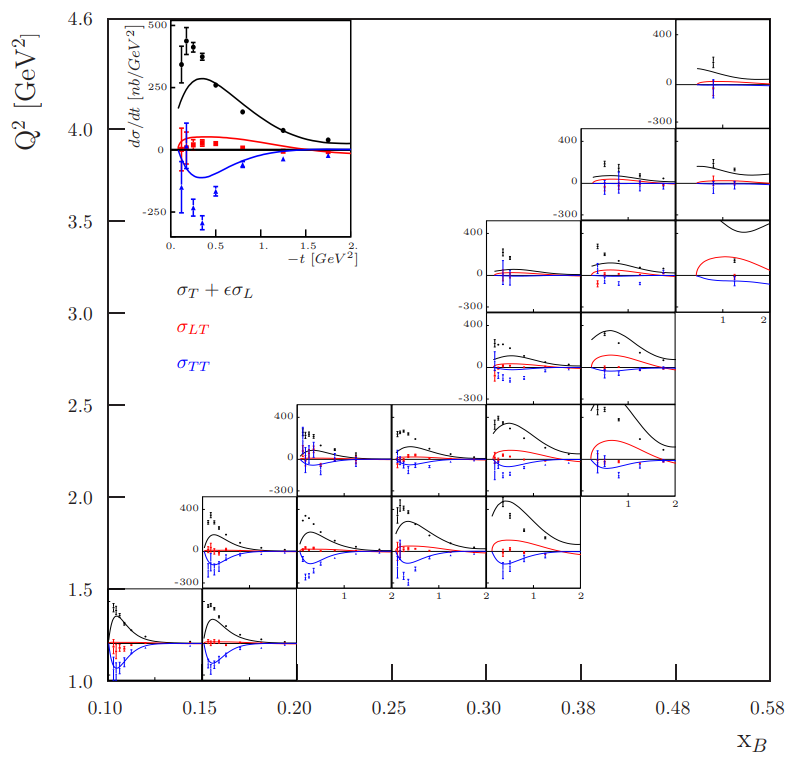
\includegraphics[width=.8\textwidth]{Pics/Goal/clas6CrossSection.png}
            \label{fig:clas6}
            \end{figure}
            
             \column{0.5\textwidth}
             \centering$Q^2$ vs. $x_B$ - CLAS12
             %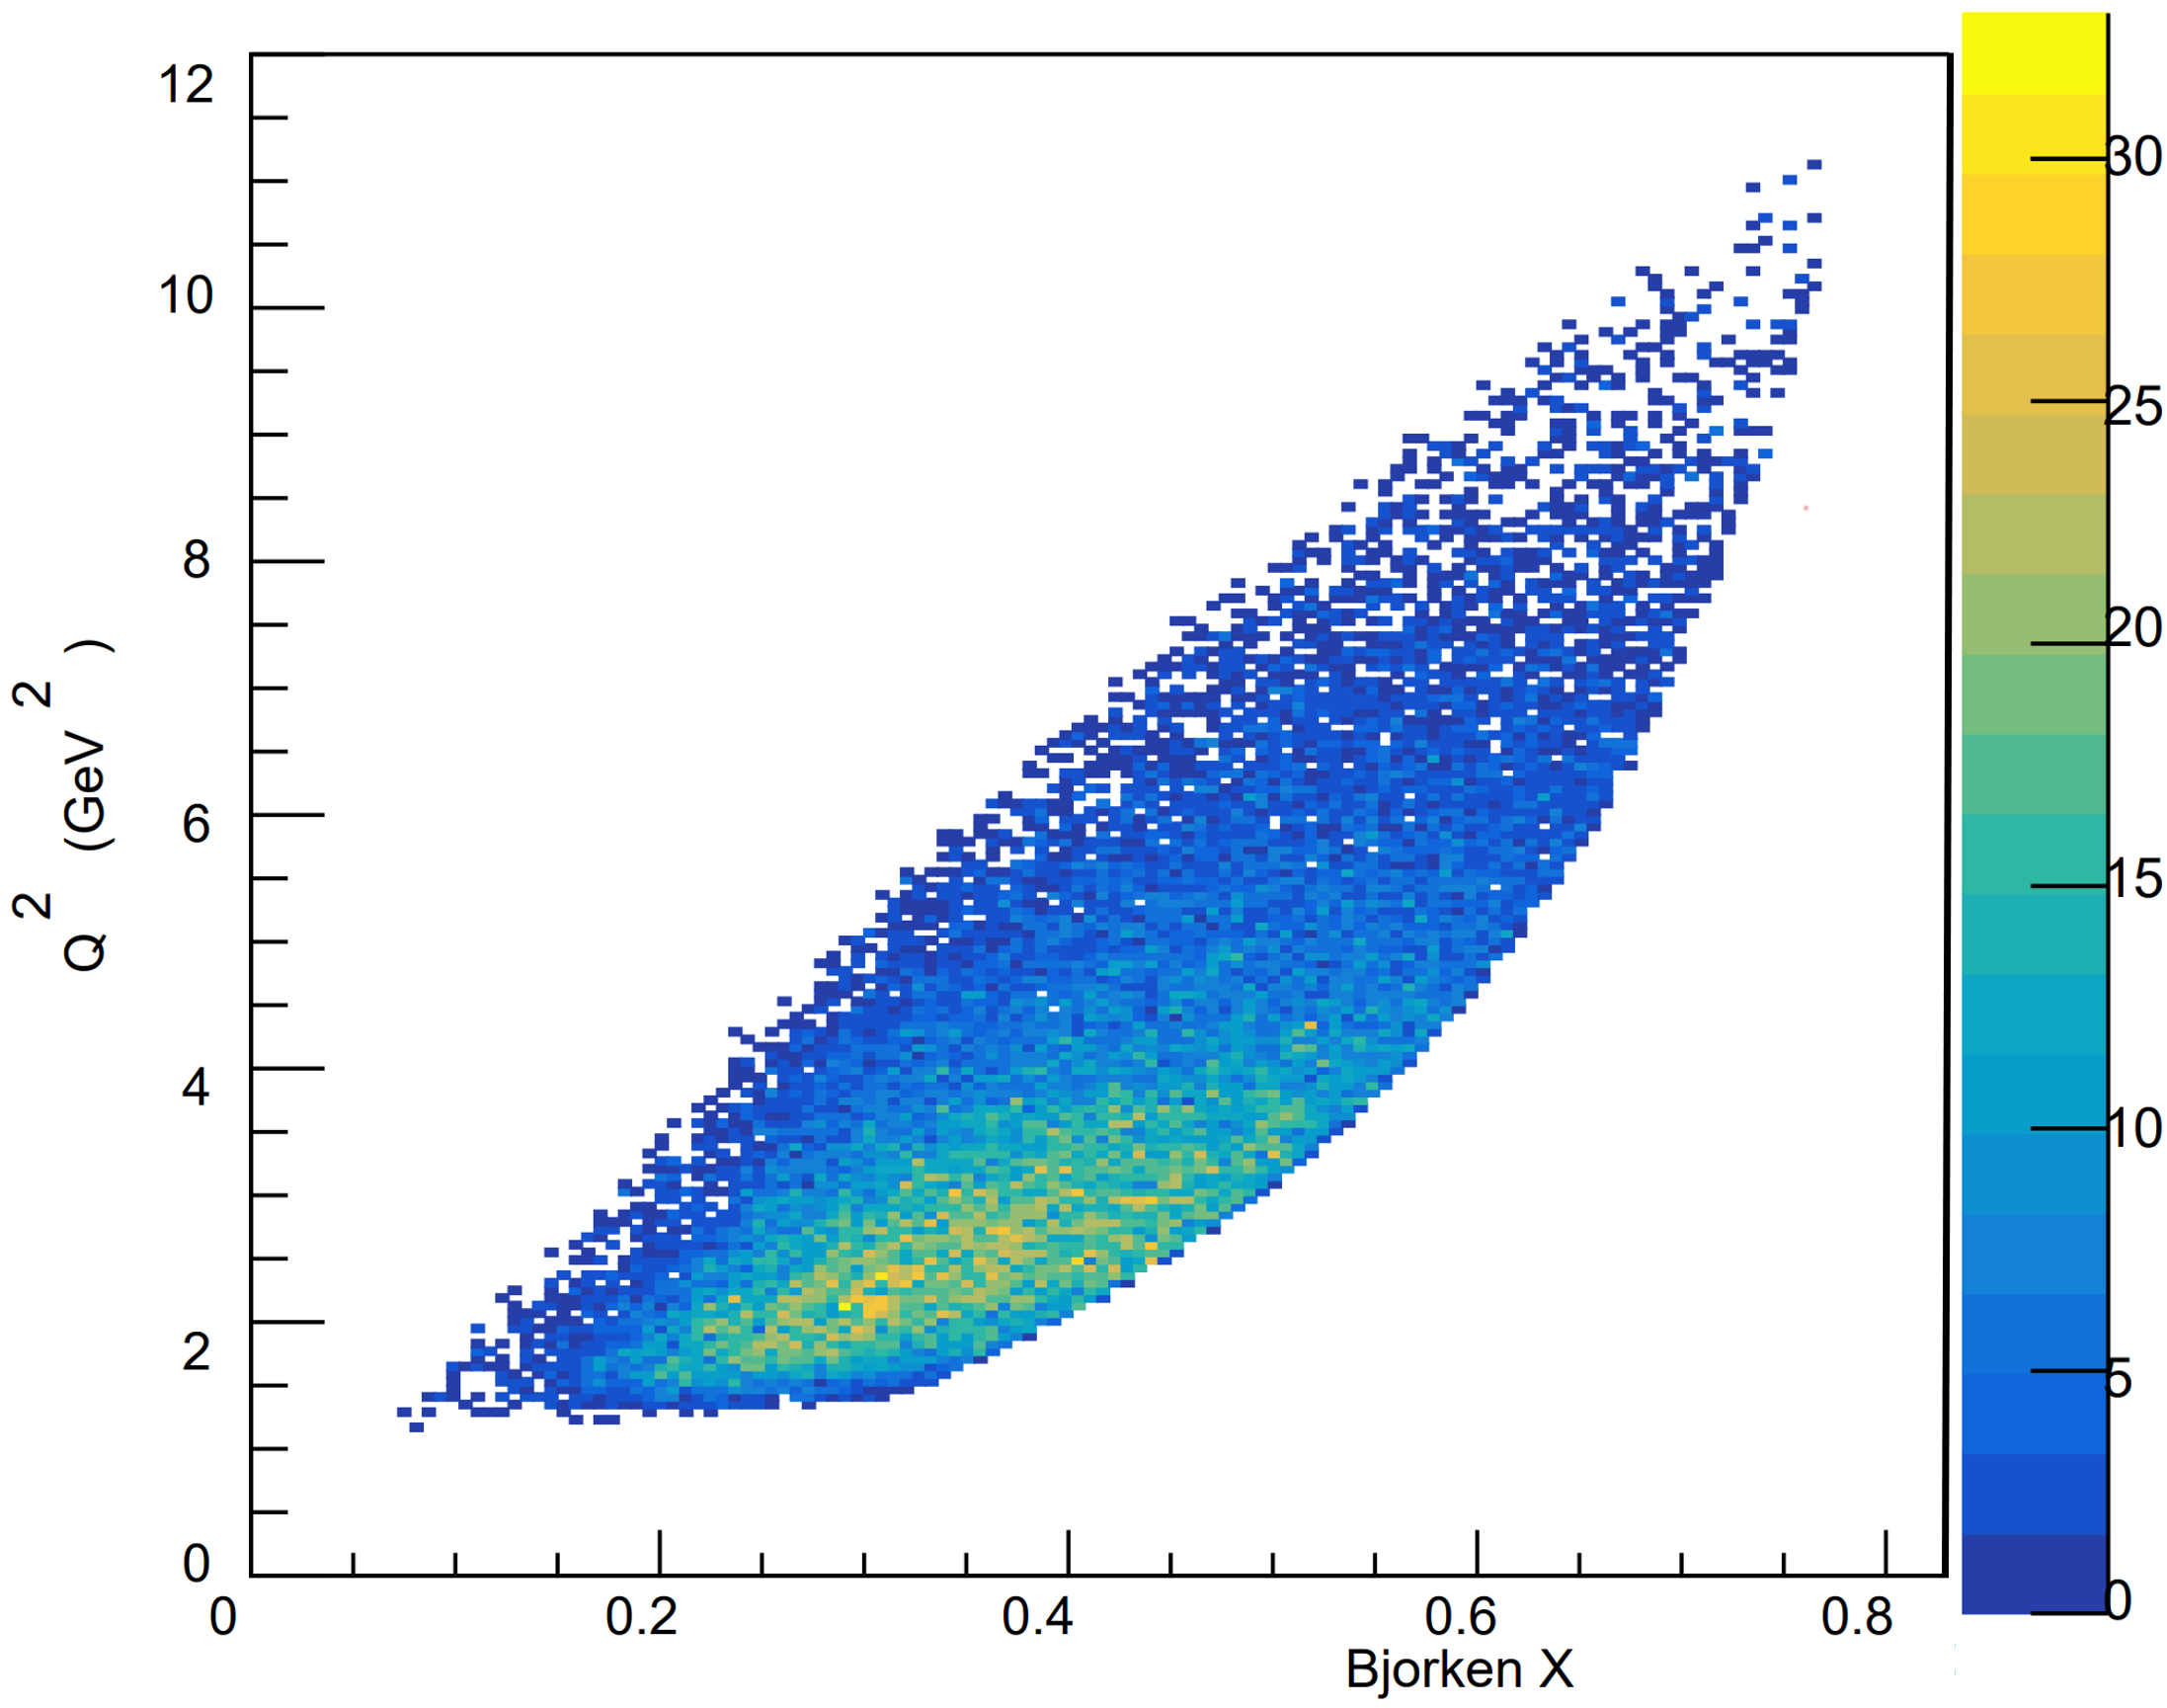
\includegraphics[width=.9\textwidth]{Pics/kinreach/bjorken_x_cropped.png}
             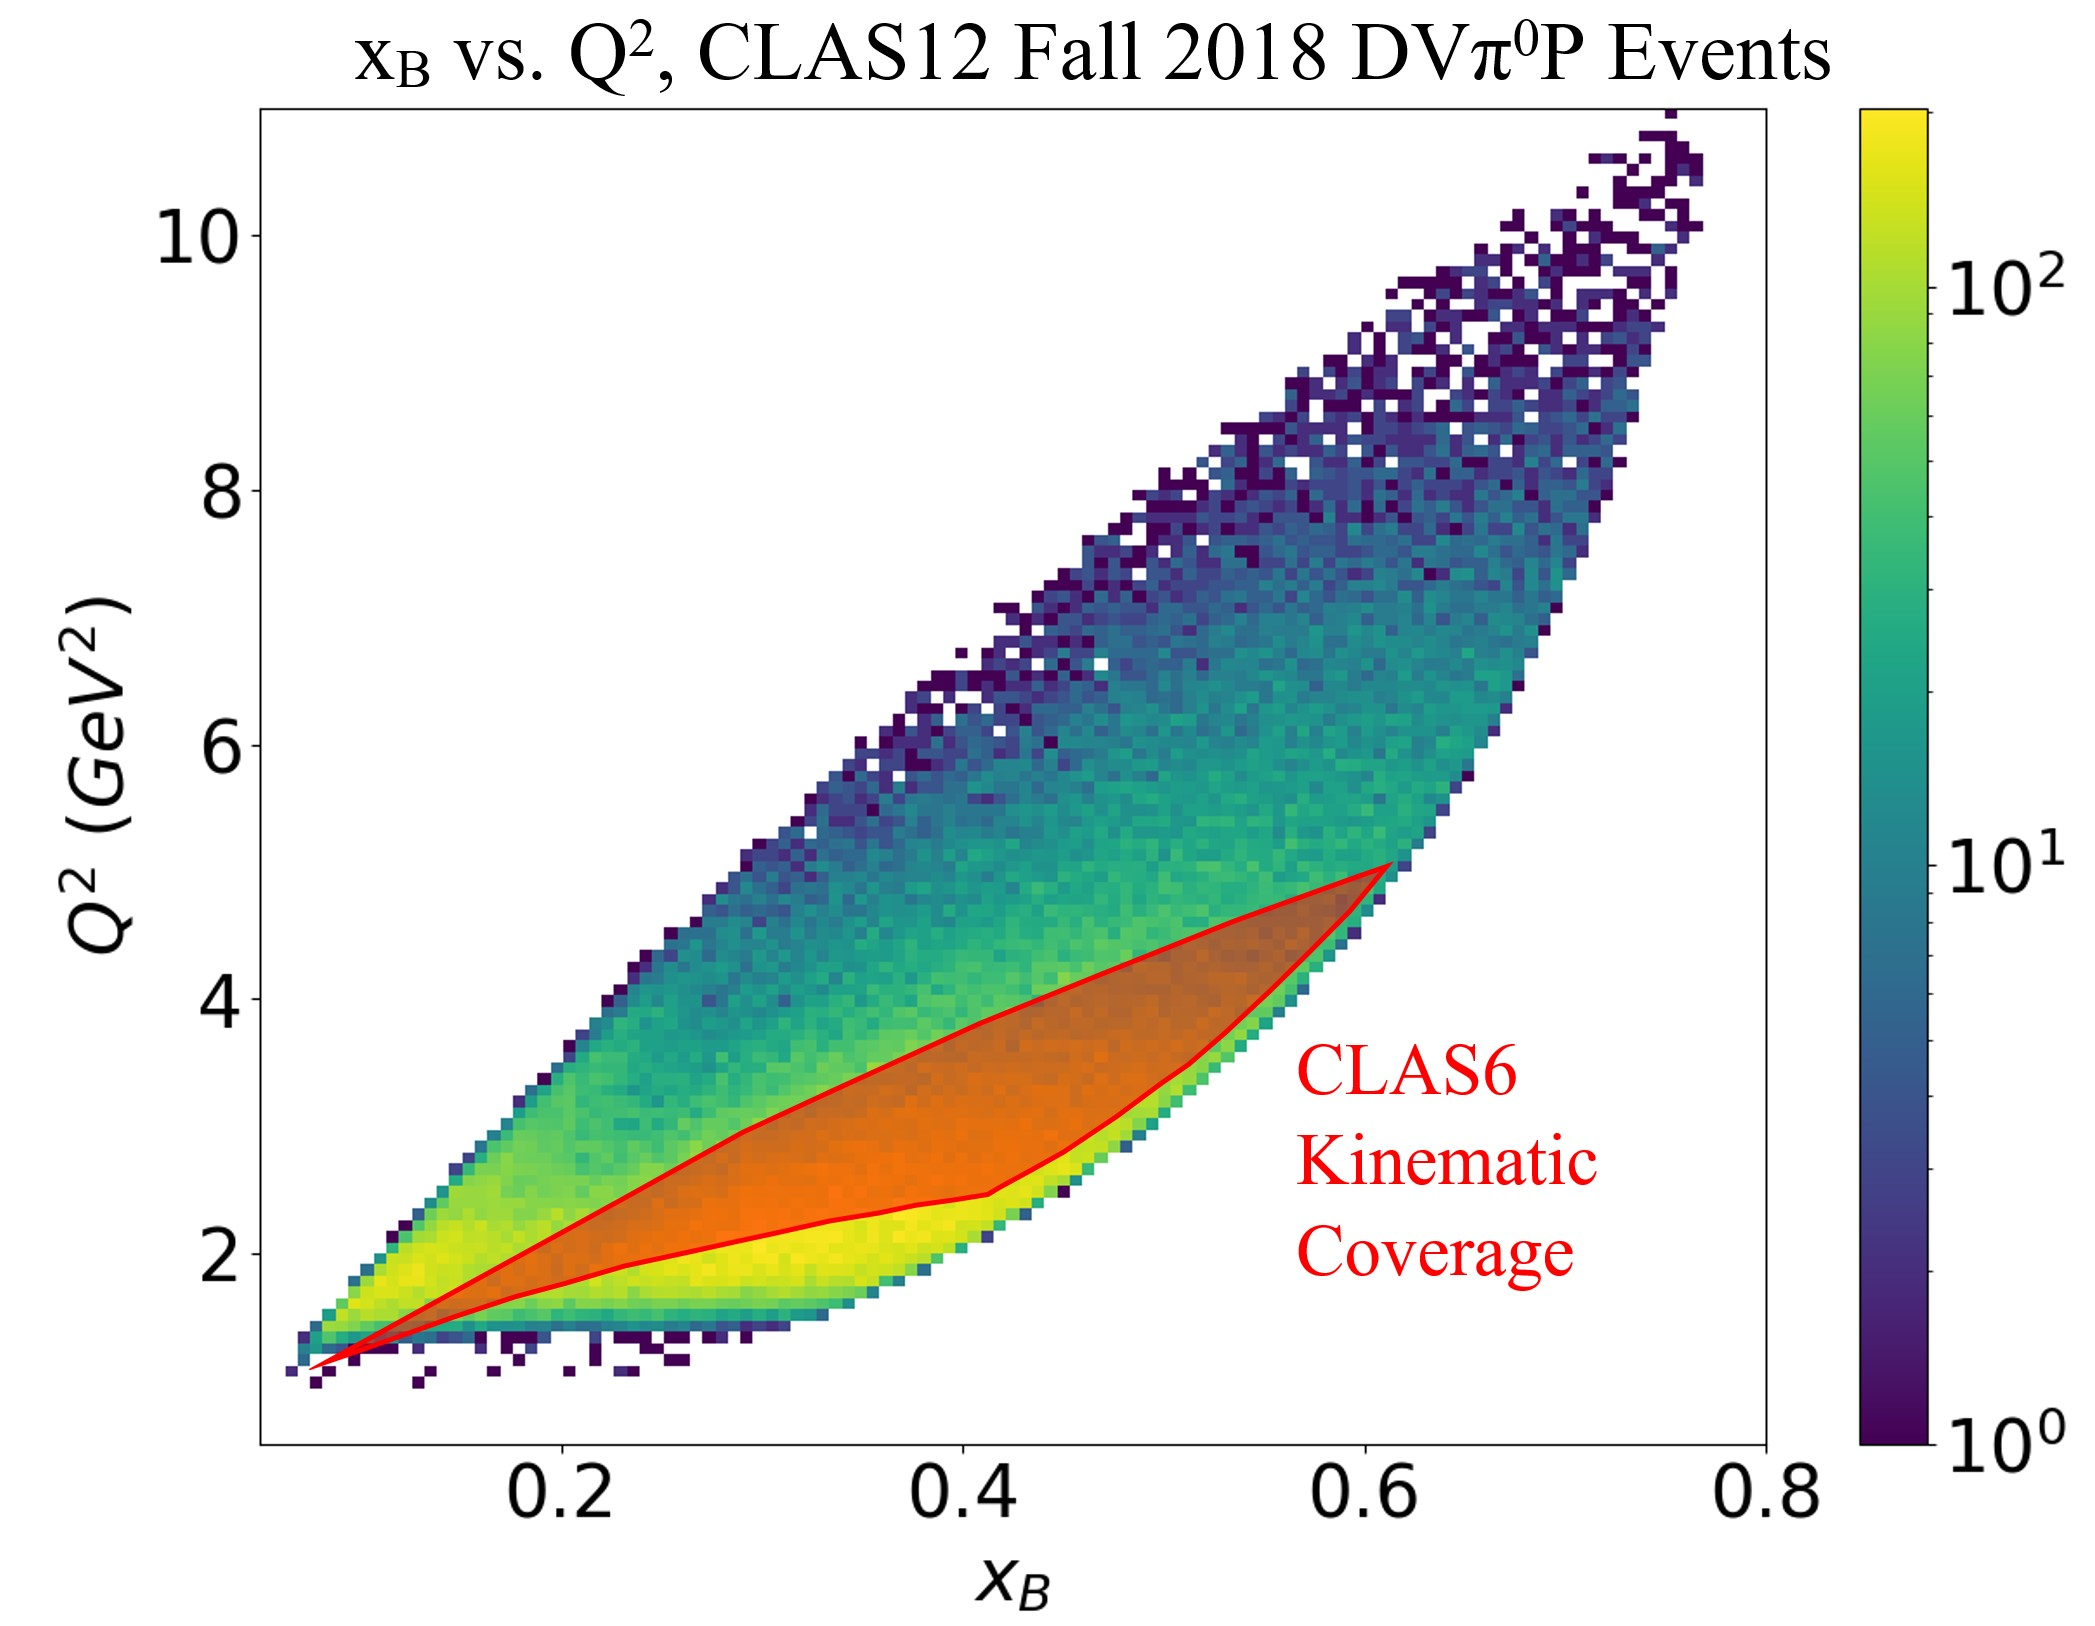
\includegraphics[trim={0 0 0 1.8cm} ,clip,width=.9725995\textwidth]{APS_2022/clas12_vs_clas6_kinematic_coverage.jpg}
    \end{columns}
    
    {\myfont{\tiny     I. Bedlinskiy et al., PRC, 90, 025205     (2014)   }}

\end{frame}



\begin{frame}{CLAS12 Detector at Jefferson Lab Hall B} \label{frame:datasets1}
        \vspace{-0.5cm}
        \begin{columns}[t, onlytextwidth]
            \column{0.5\textwidth}
                %\vspace{1cm}
                \begin{figure}[t!]
                    %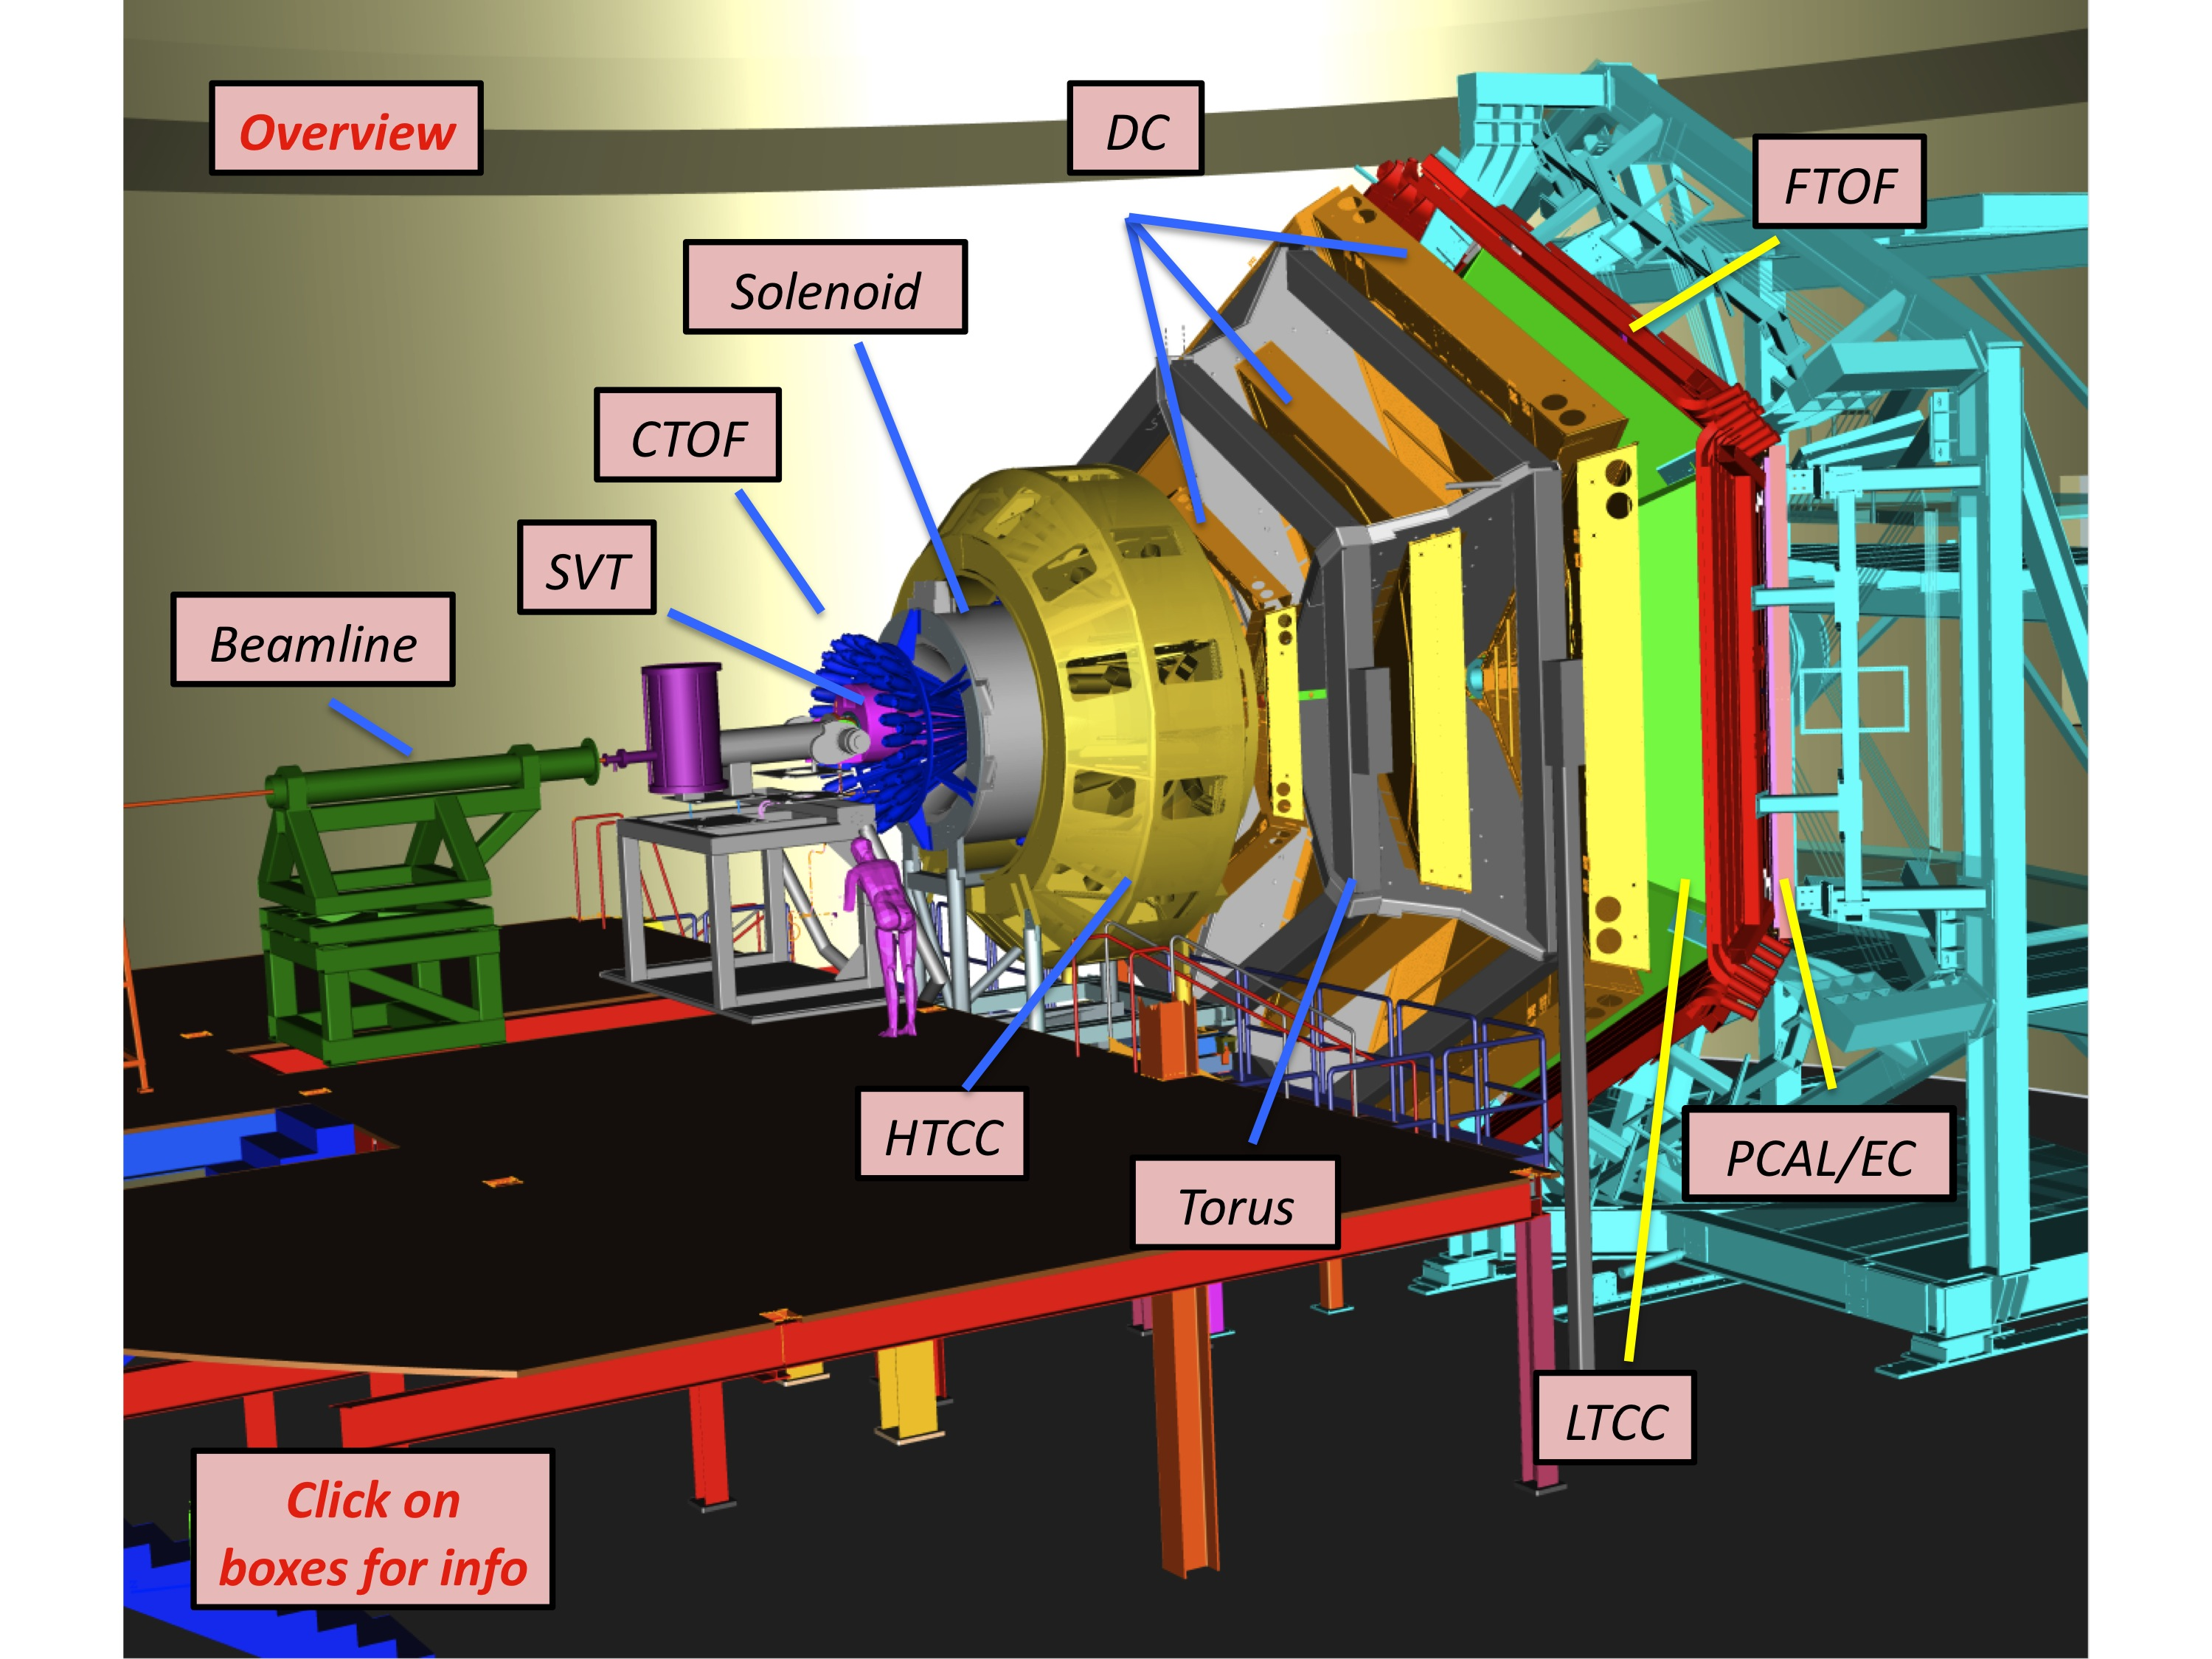
\includegraphics[height=\dimexpr0.5\textheight-0.5in]{Pics/dnp/clas12-overview.jpg}
                    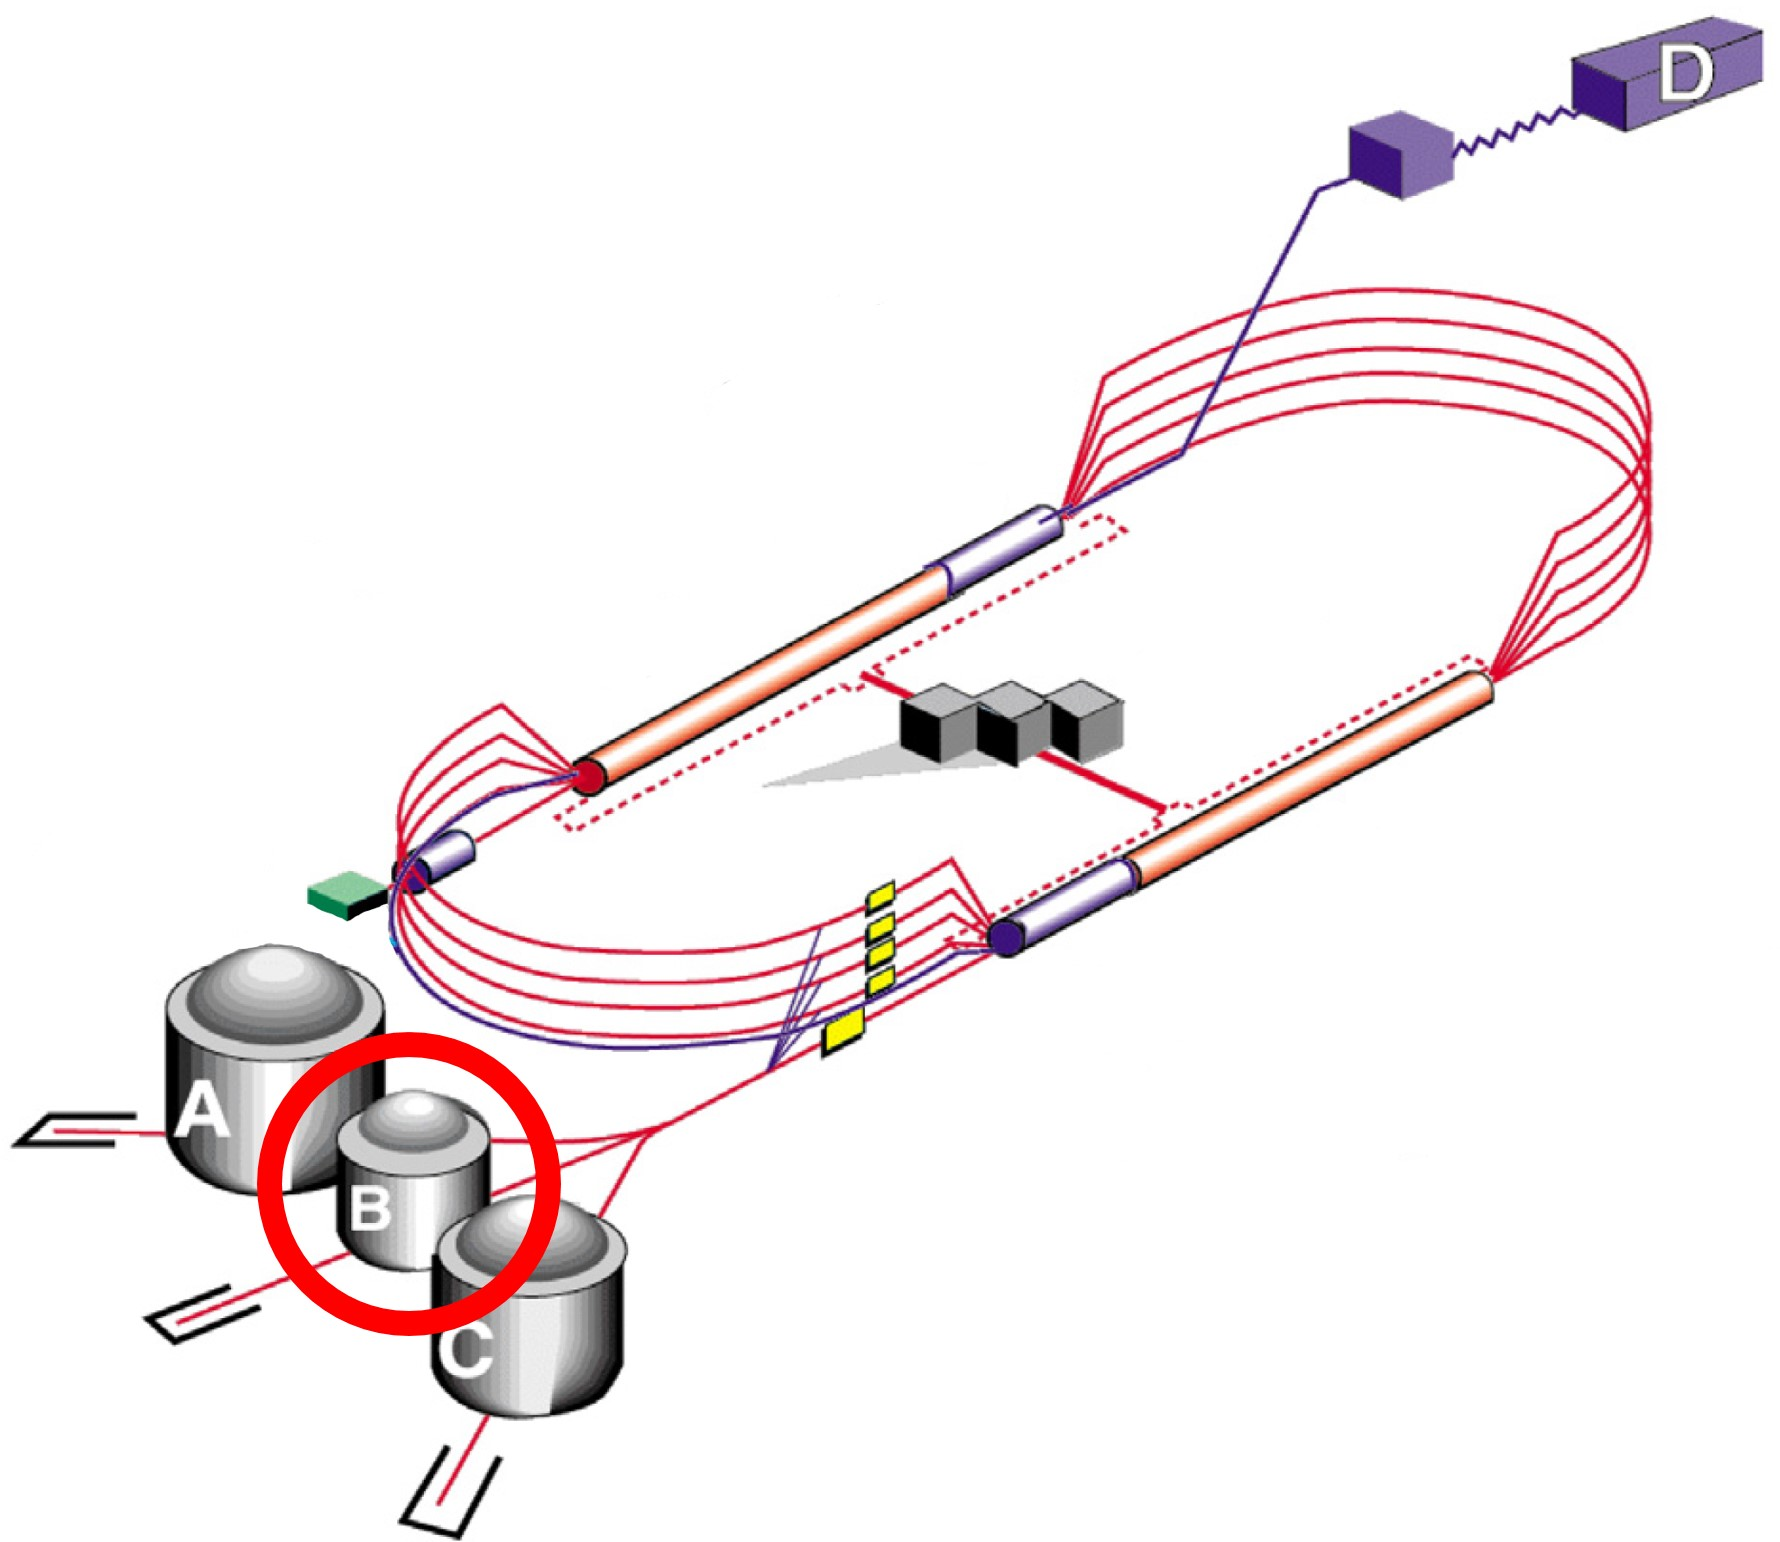
\includegraphics[width=.6349\textwidth]{DNP/jlab_hall_b_circled.jpg}
                    
                    
                \end{figure}
                \vspace{-0.45cm}
                  \begin{itemize}
                    \setlength\itemsep{1em}
                    \item CEBAF Large Acceptance Spectrometer in Jefferson Lab Hall B
                    \item 10.6 GeV, $\sim$ 50 nA e$^-$ 86\% polarized beam on unpolarized LH$_2$ target
                    \end{itemize}
                    
            \column{0.5\textwidth}
                \begin{figure}[t!]
                    %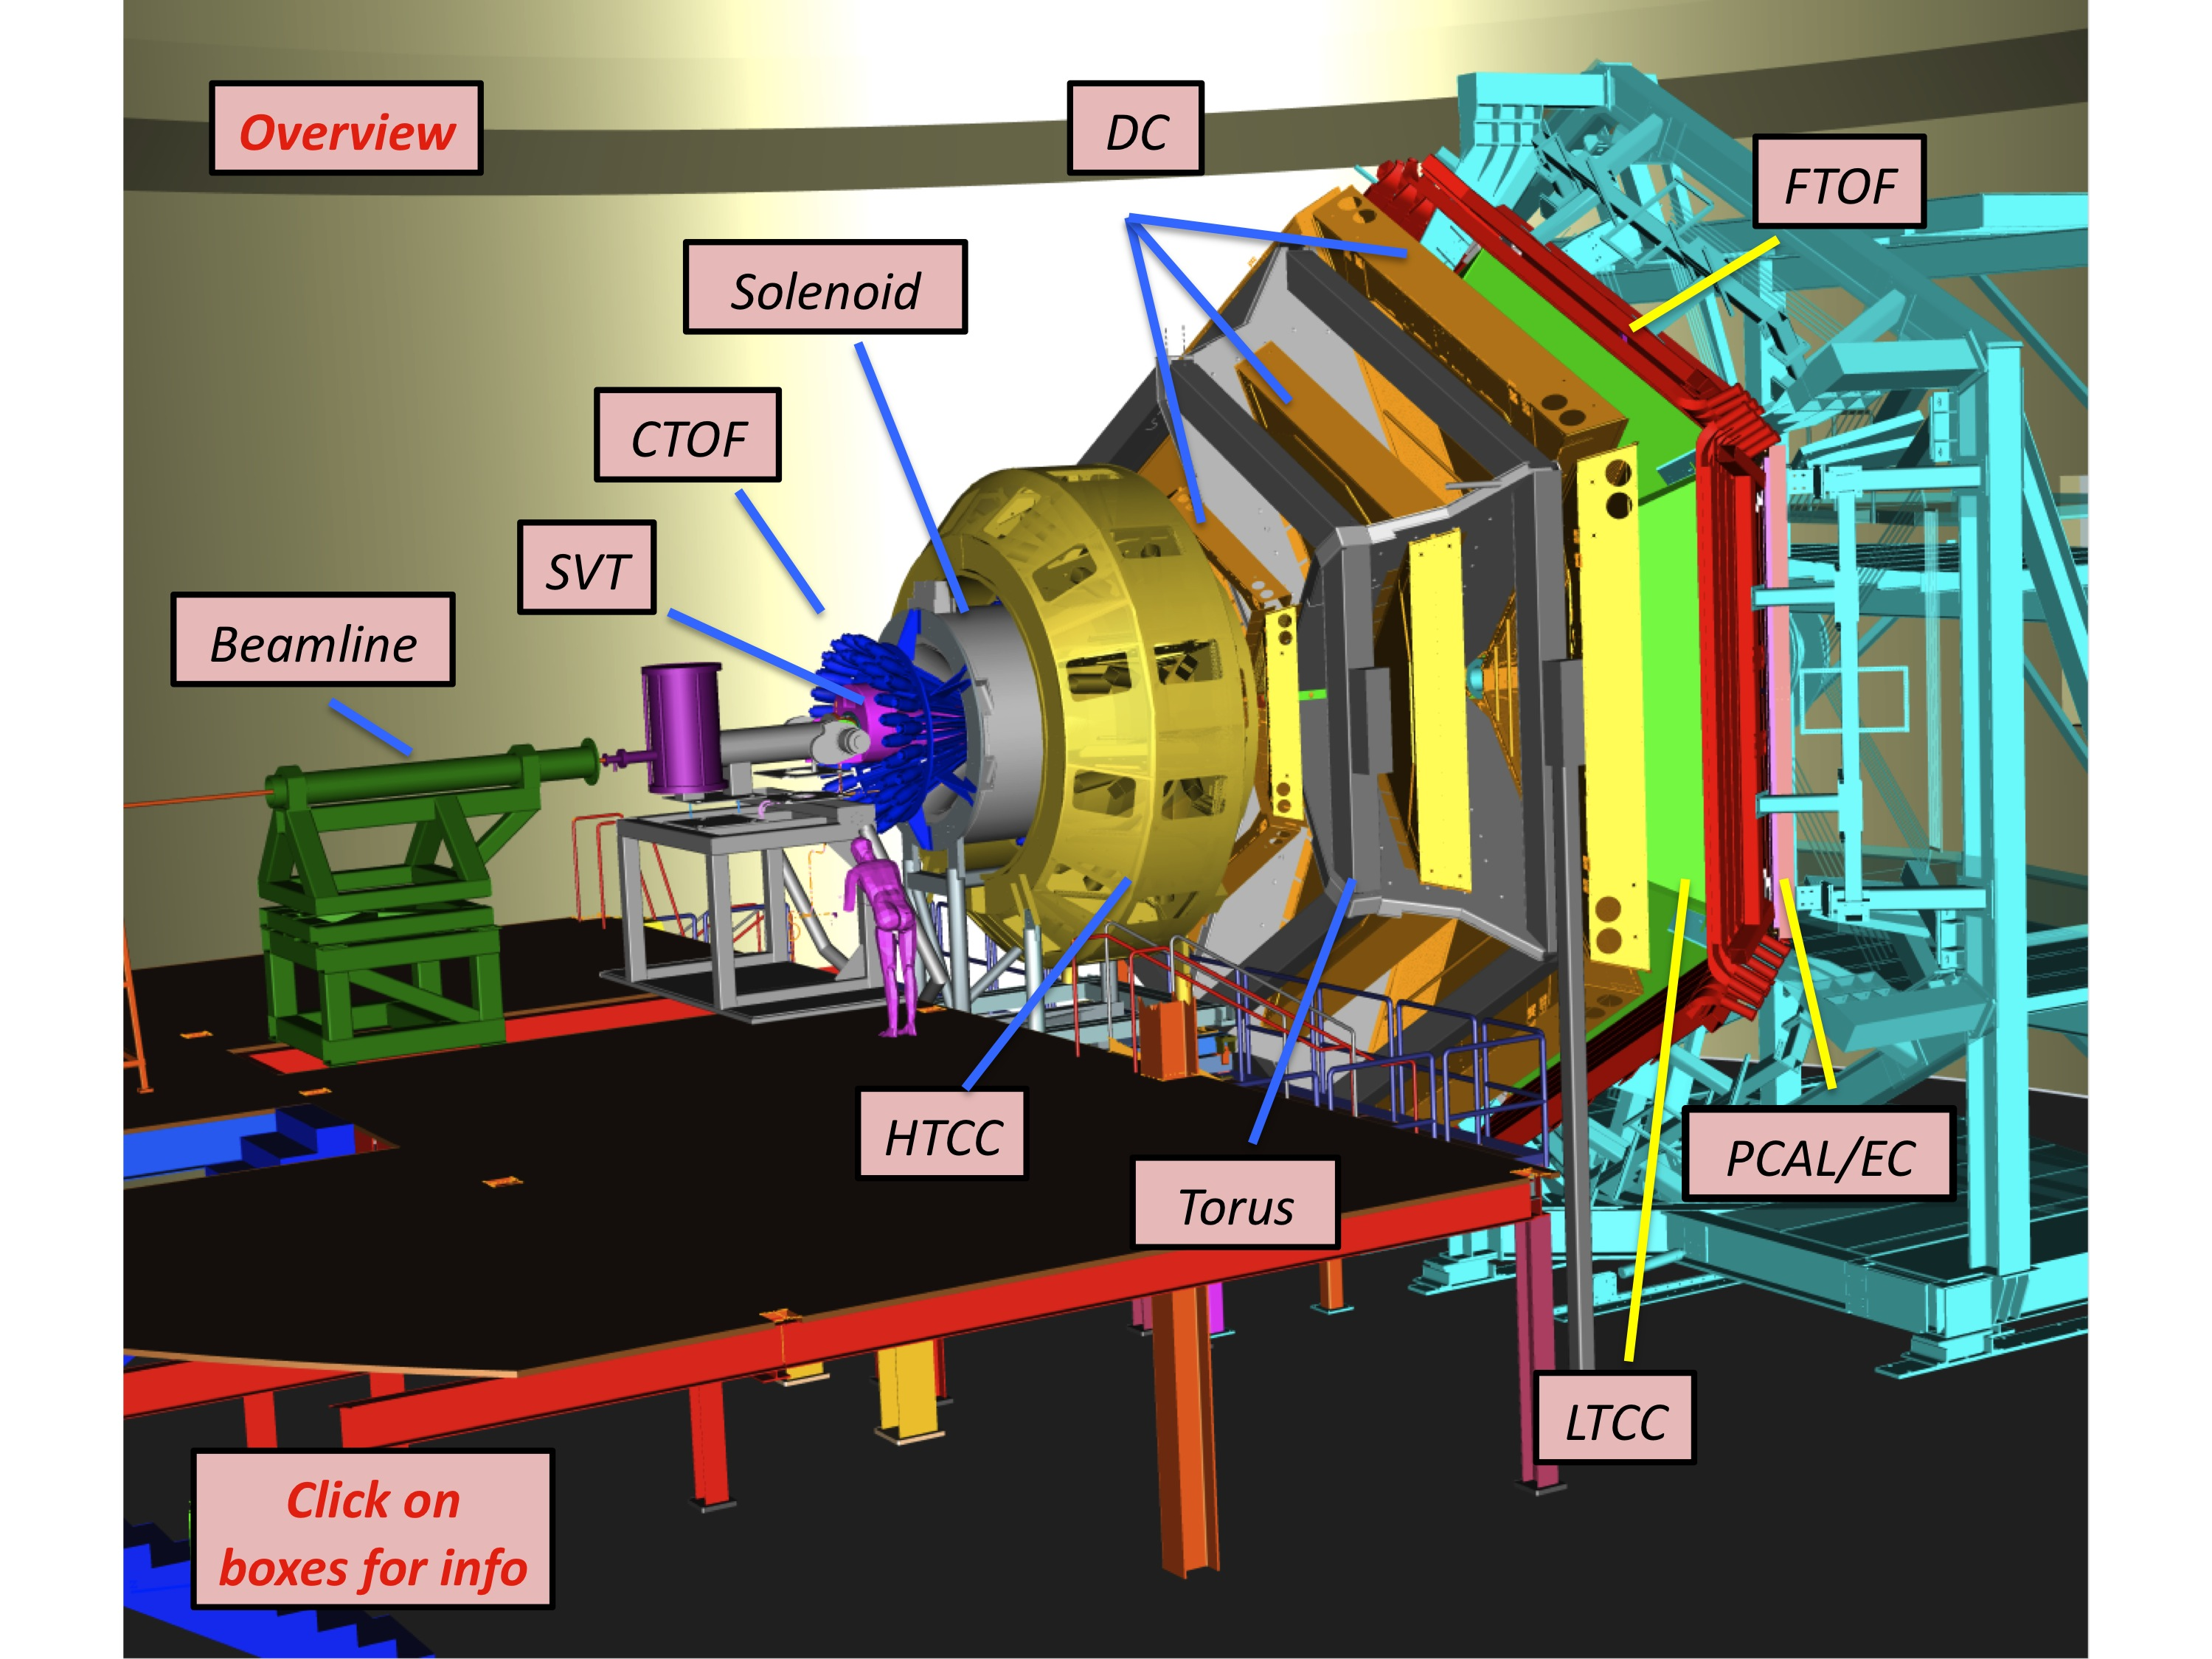
\includegraphics[height=\dimexpr0.5\textheight-0.5in]{Pics/dnp/clas12-overview.jpg}
                    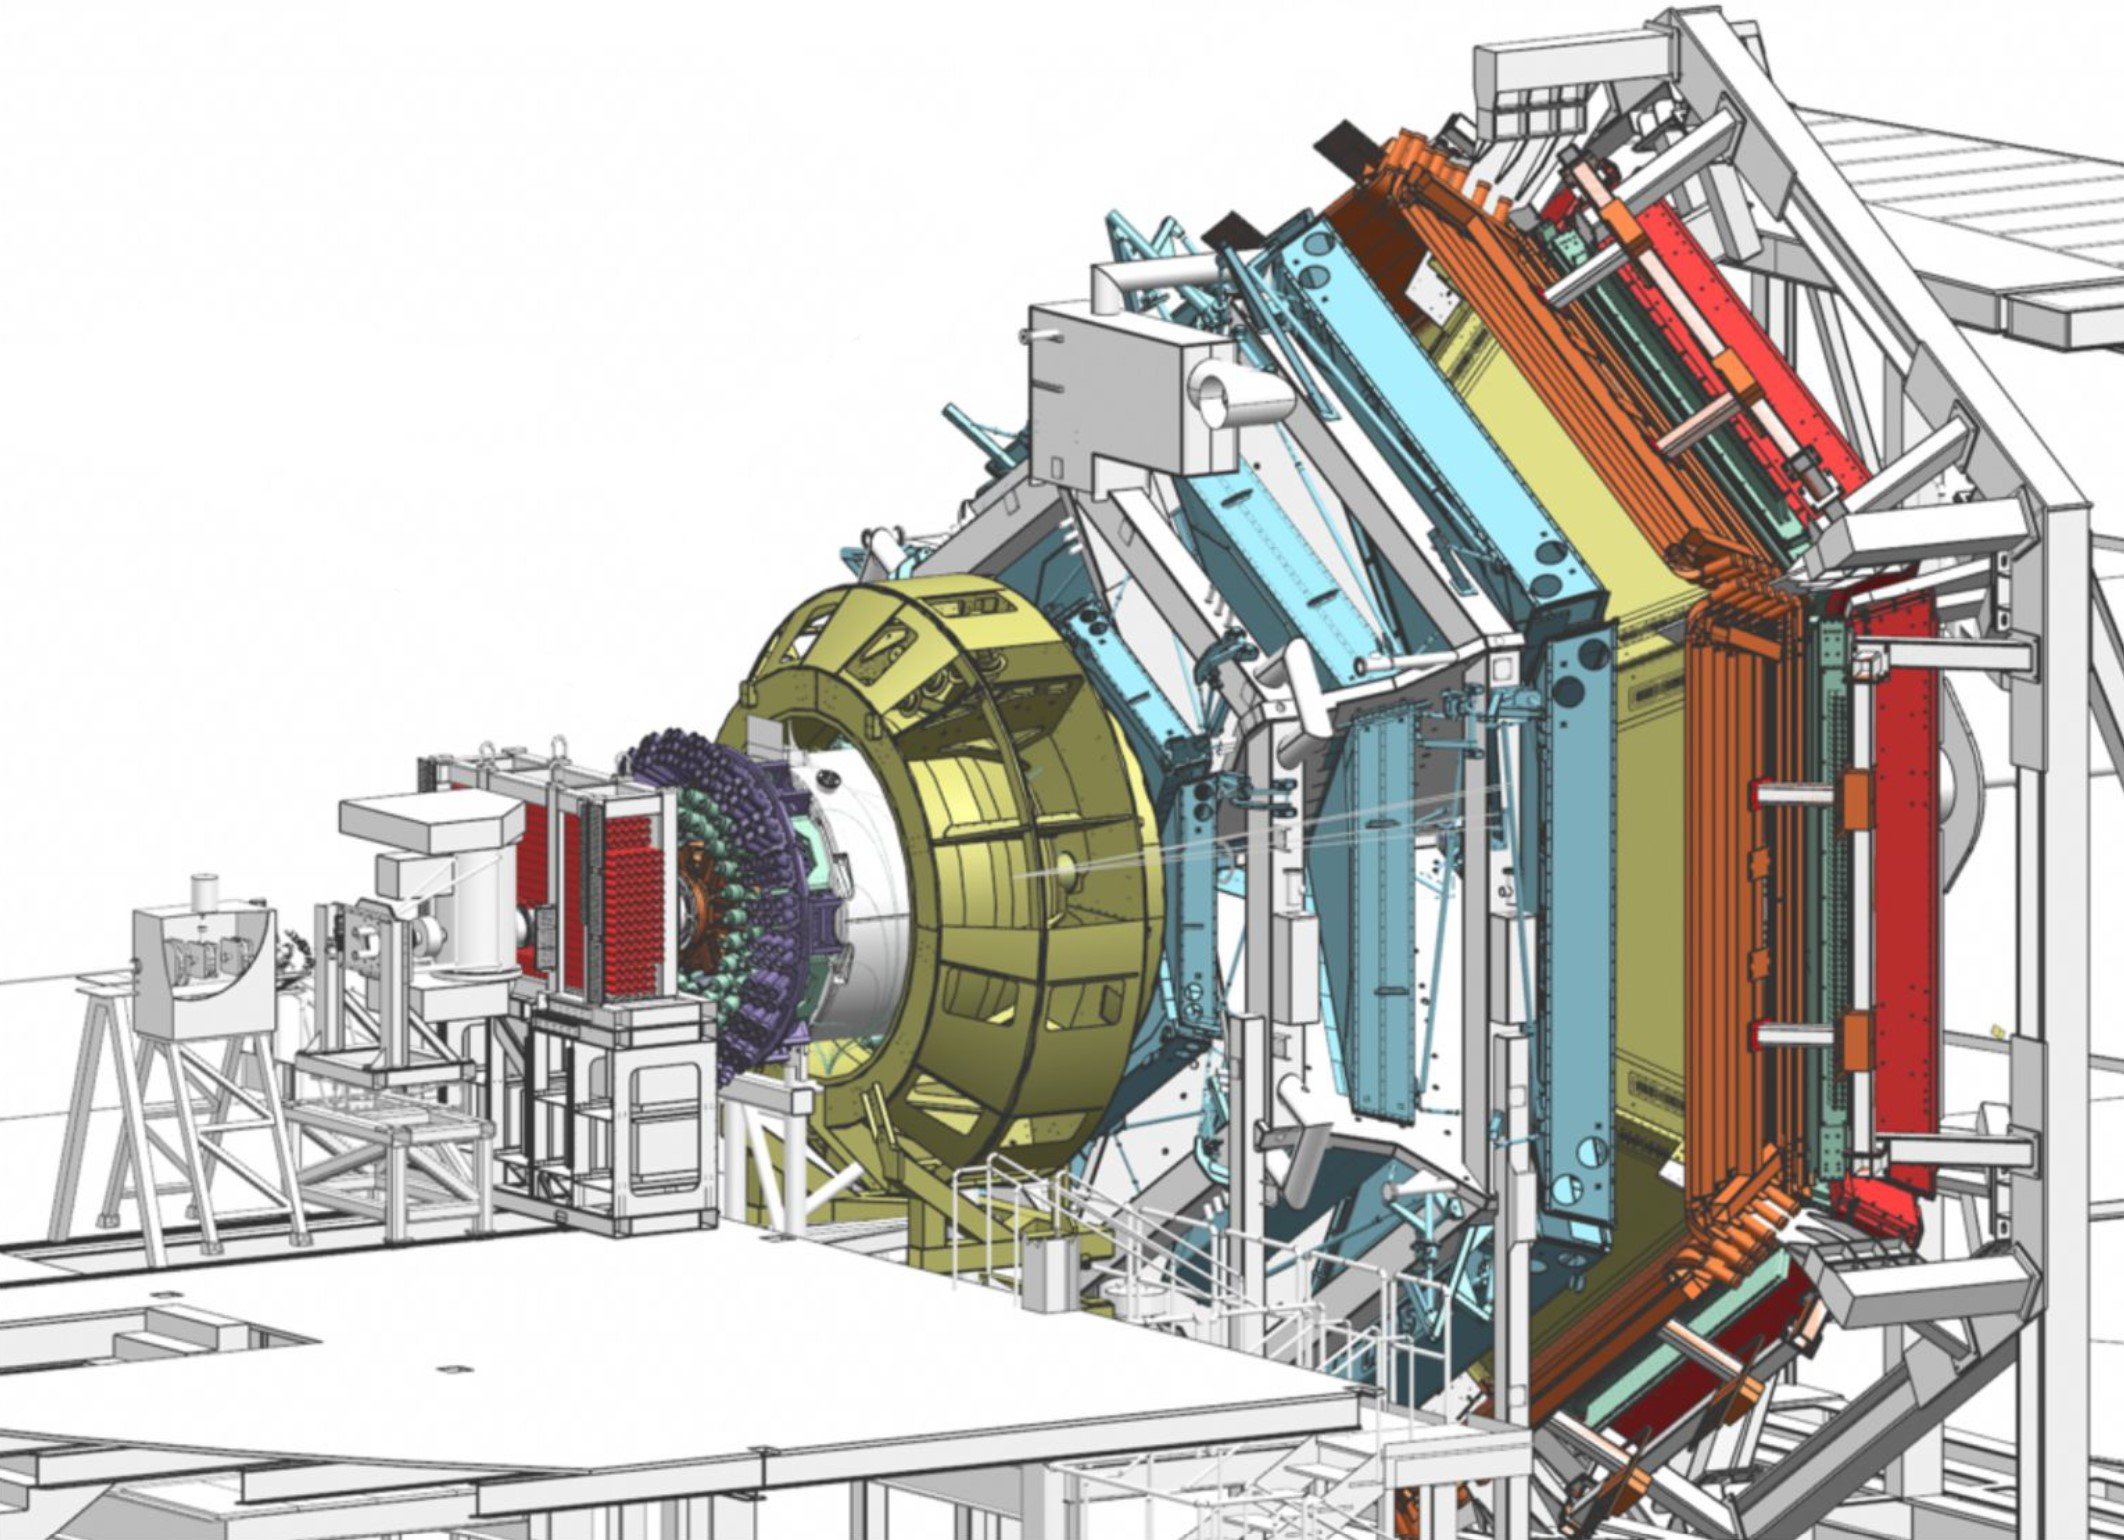
\includegraphics[width=.765899\textwidth]{DNP/CLASdetector.jpg}
                    
                    
                \end{figure}
                \vspace{-0.45cm}
                \begin{itemize}
                    \setlength\itemsep{1em}

                    \item Large Acceptance:\\
                     \begin{itemize}
                            \item $\sim$ 2$\pi$ coverage in $\phi$\\
                        \item  $5^\circ$ - $125^\circ$ coverage in $\theta$
                        \item Full 4 particle final state reconstruction for this process
                    \end{itemize}
                    
                    
                \end{itemize}
                \vspace{0.3cm}
                {\myfont{\tiny V. Burkert et al., NIMA, 959, 163419 (2020) }}
        \end{columns}
\end{frame}    


\begin{frame}{Experiment Layout And Particle Detection} \label{frame:datasets}
\vspace{-0.5cm}
        \begin{columns}[t, onlytextwidth]
            \column{0.55\textwidth}
                \begin{itemize}
                    \setlength\itemsep{.35em}
                    \item 6-fold symmetric Forward Detector ($\theta < \sim 40 ^{\circ}$) with torodial field
                     \begin{itemize}
                    \setlength\itemsep{.25em}
                        \item Cherenkov Counters
                        \item Drift Chambers
                        \item Time-of-Flight Detectors
                        \item EM Calorimeters
                    \end{itemize}
                      \item Central Detector ($\sim40 < \theta < \sim 125 ^{\circ}$) inside solenoid
                     \begin{itemize}
                    \setlength\itemsep{.25em}
                        \item Silicon Vertex Tracker
                        \item Micromegas
                        \item ToF Detector

                    \end{itemize}
                    
                    \item Forward Tagger, Backward Angle Neutron Detector
                    \item Faraday Cup for luminosity measurement
                
            
                \end{itemize}
            
                \vspace{0.1cm}
                
            \column{0.45\textwidth}
                %\vspace{1cm}
                \vspace{0.3cm}
                \begin{figure}[t!]
                    %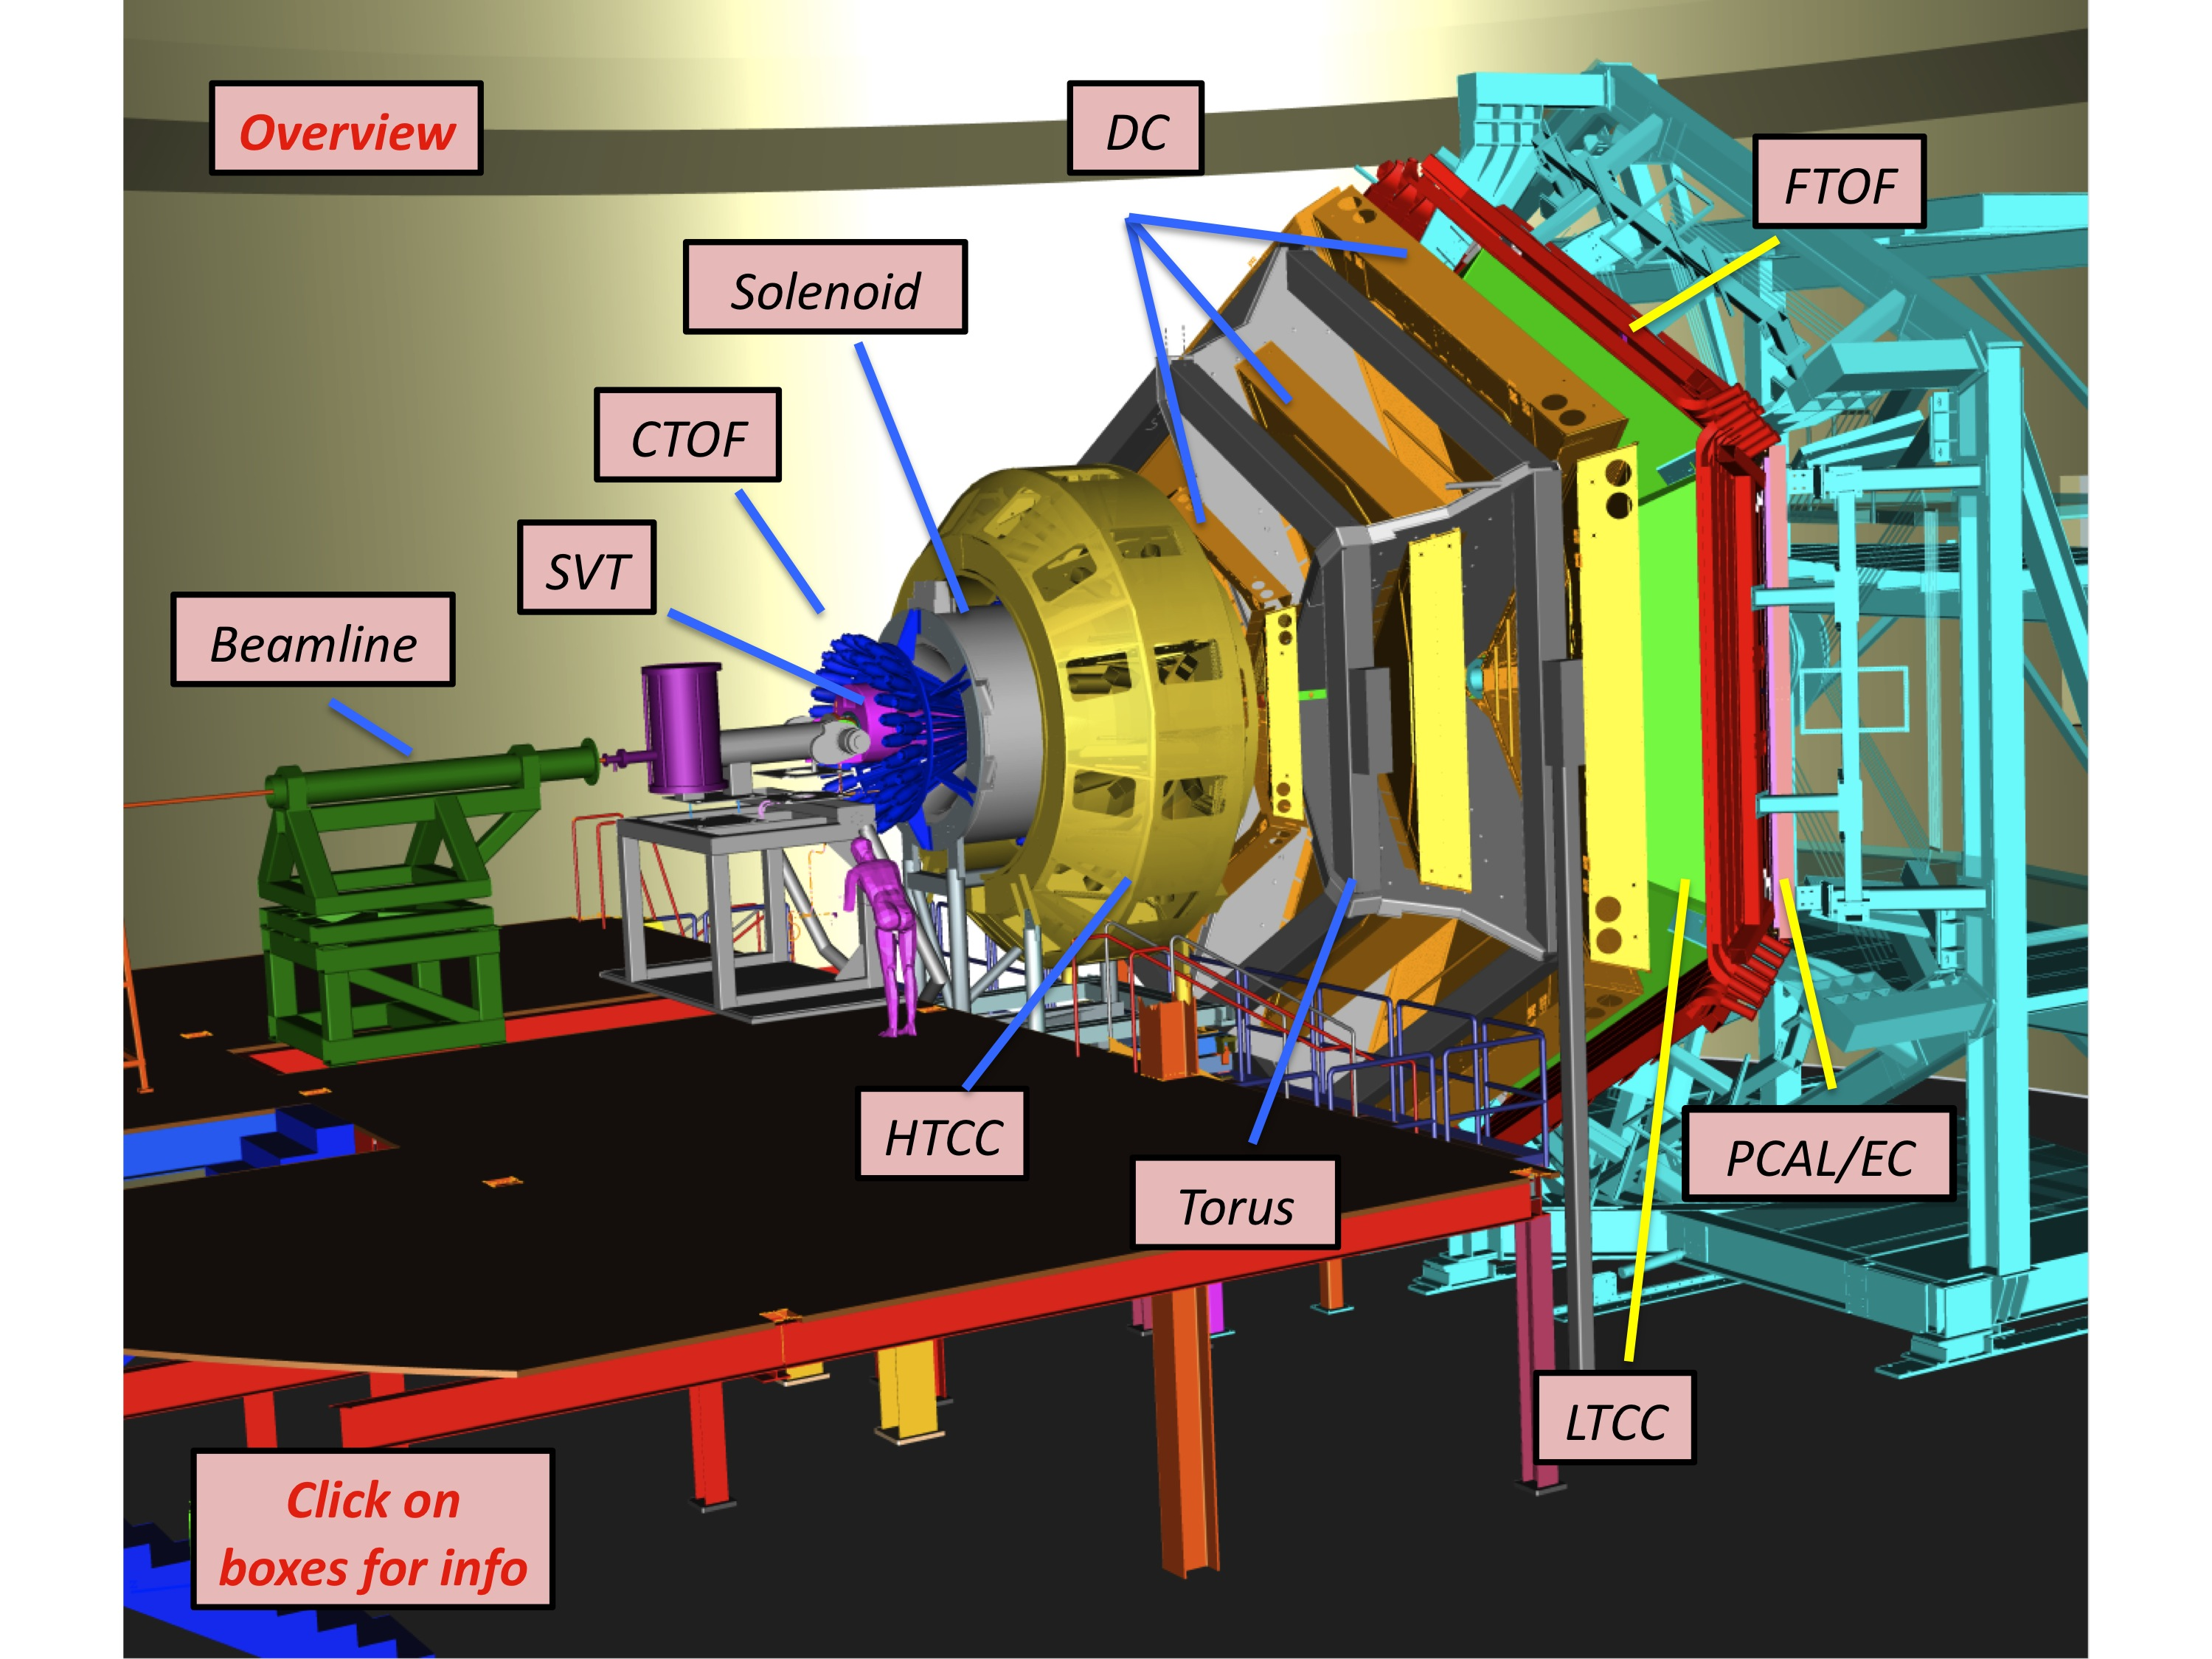
\includegraphics[height=\dimexpr0.5\textheight-0.5in]{Pics/dnp/clas12-overview.jpg}
                    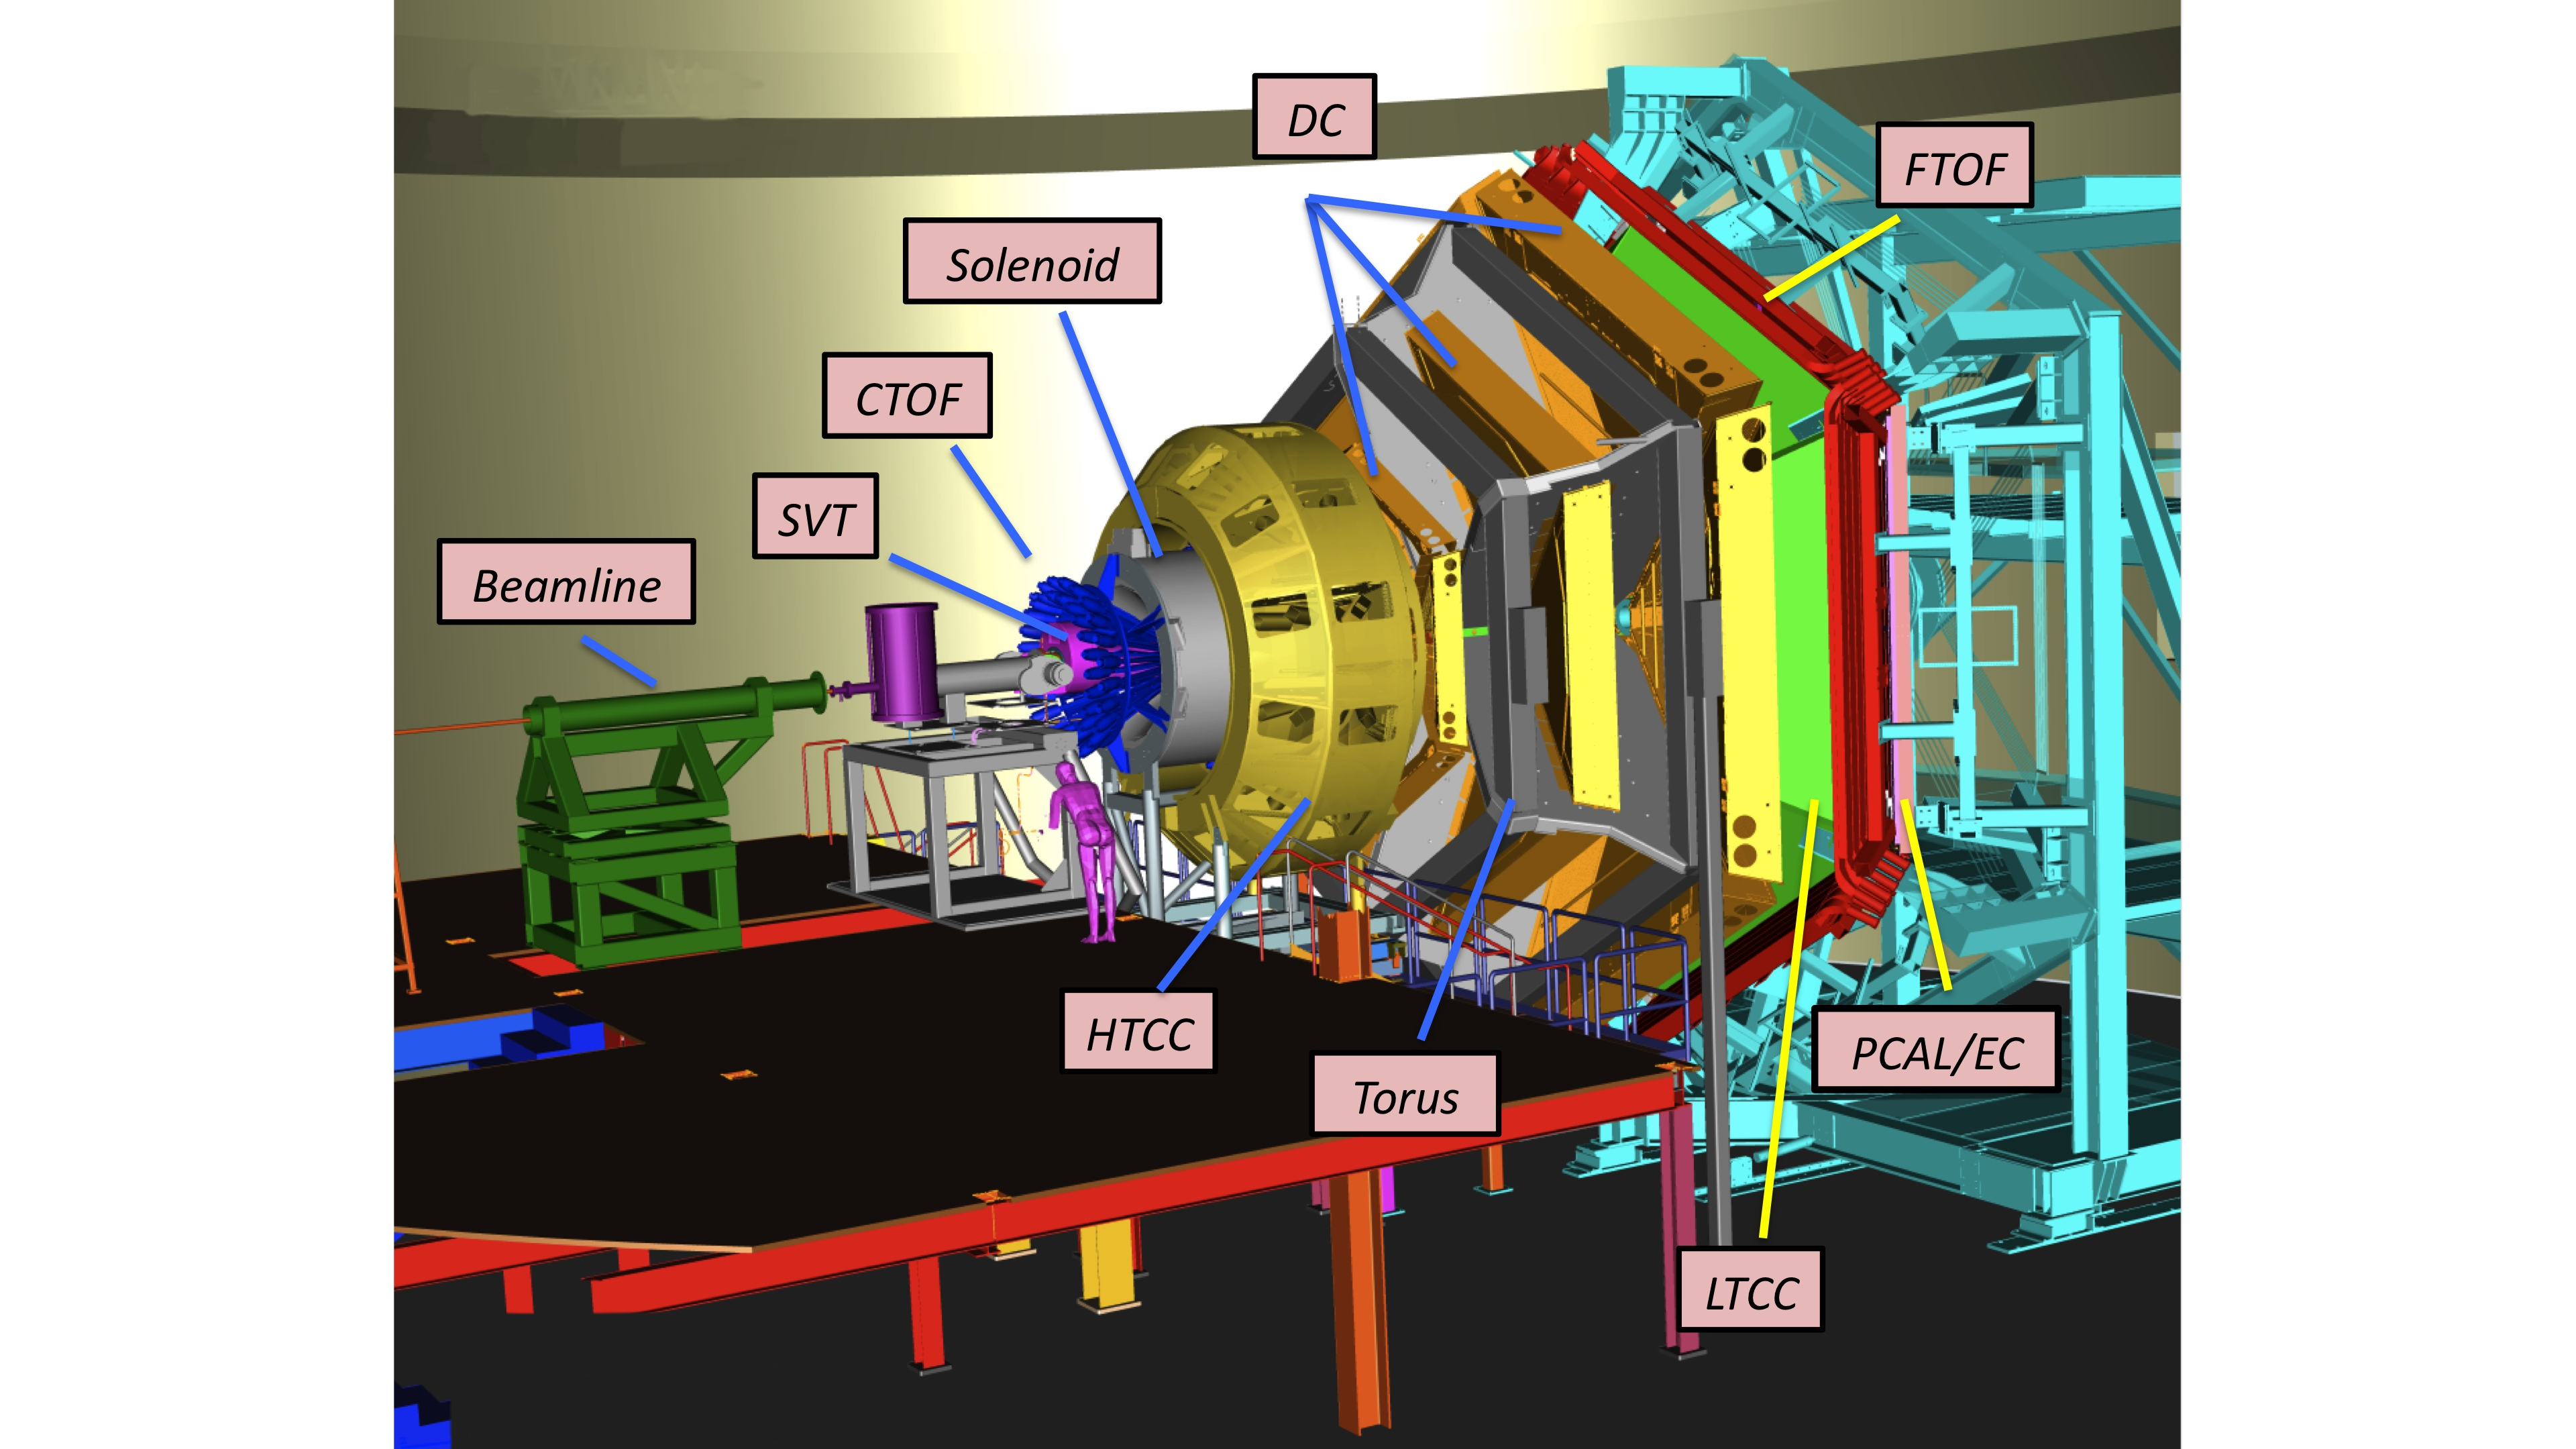
\includegraphics[trim={8cm 1cm  8cm 1cm},width=.899\textwidth]{DNP/jlab_clas_layout_1.png}
                    

                    
                \end{figure}
                \begin{itemize}
                    \setlength\itemsep{.35em}
                    \item This analysis examines data taken in Fall 2018
                    \end{itemize}
                {\myfont{\tiny V. Burkert et al., NIMA, 959, 163419 (2020) }}
        \end{columns}
\end{frame}    




\begin{frame}{Analysis Overview: Components of Cross Section}

                %\textcolor{white}{blank space}
                \centering 
                %#---------------------------------------------
                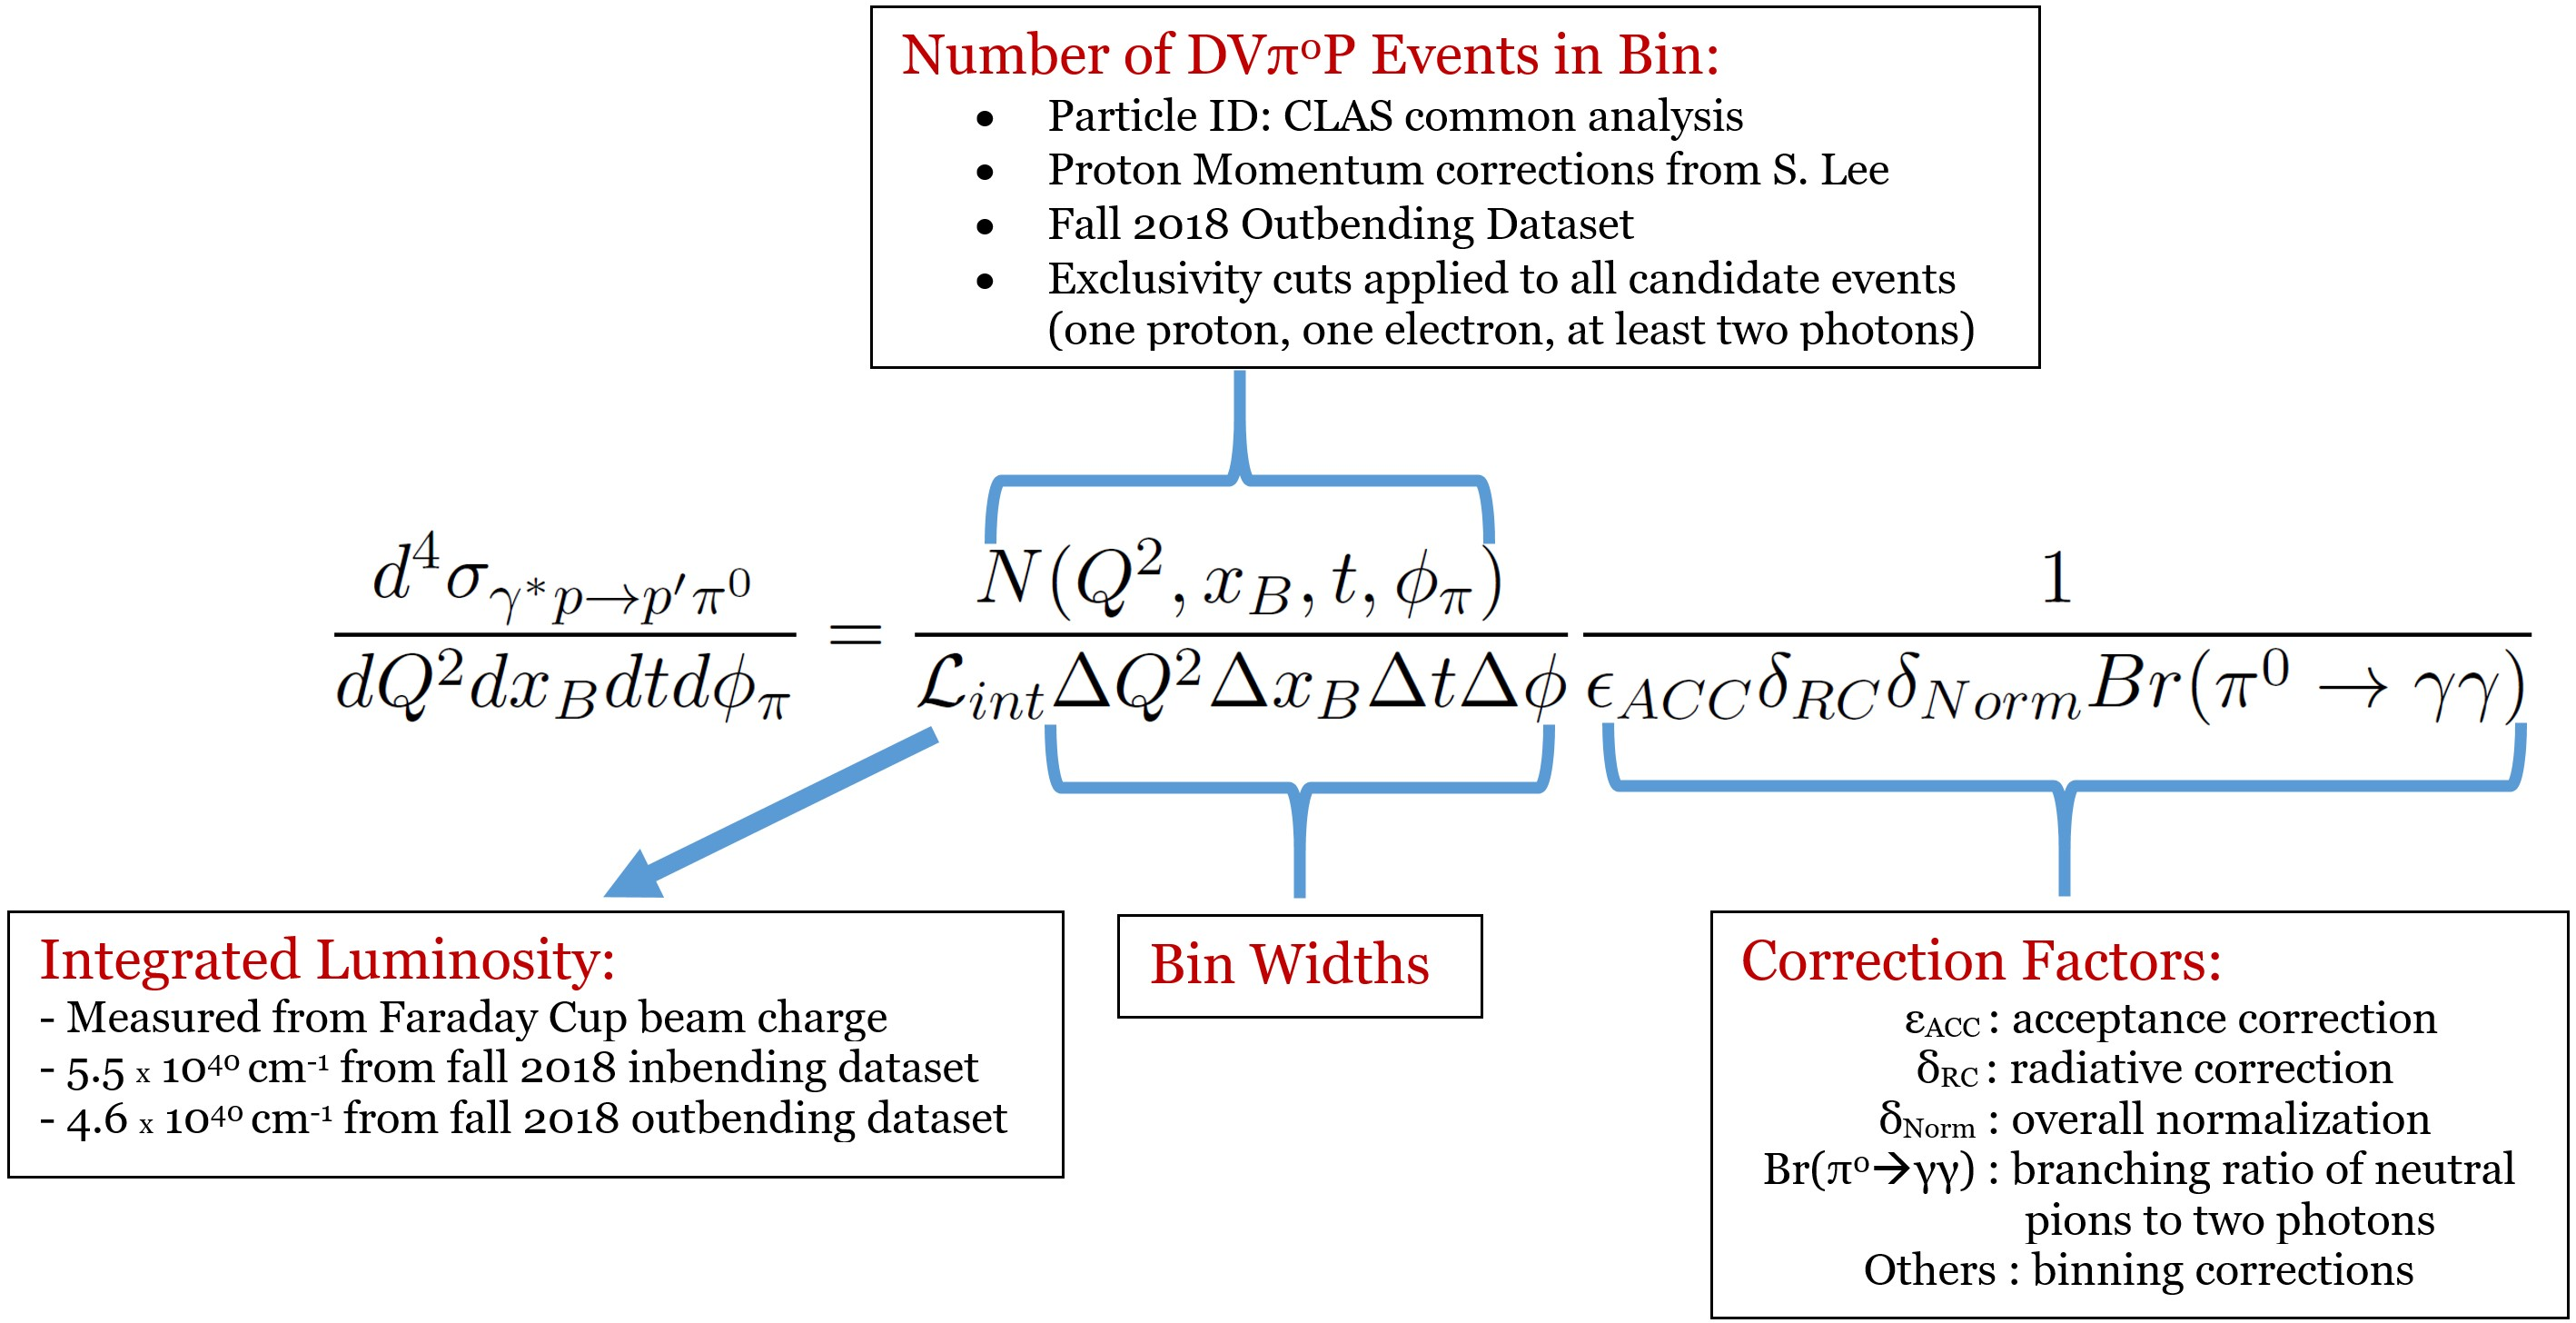
\includegraphics[trim={0 0  0 0cm} ,clip,width=.91725995\textwidth]{extra/steps3.jpg}

\end{frame}


\begin{frame}{Event Selection - Particle Identification and Exclusivity Cuts}

        
        \begin{columns}[c]
           \begin{column}{0.35\textwidth}
            \centering \textbf{\underline{Particle Kinematics}}
                %\vspace{1cm}
                \begin{itemize}
                    \item Electron
                        \begin{itemize}
                            \item Cherenkov Counter (PID)
                            \item Drift Chamber (momentum)
                            \item Time-of-flight (PID)
                            \item EM Calorimeter (energy)
                        \end{itemize}
                    \item Proton
                        \begin{itemize}
                            \item Time-of-flights (PID)
                            \item Micromegas, SVT, DCs (momentum)
                        \end{itemize}
                    \item Neutral Pion
                        \begin{itemize}
                            \item EM Calorimeter ($\gamma_1, \gamma_2$)
                            \item $ |M_{\pi^0} - M_{\gamma\gamma}| <$ 40 MeV
                        \end{itemize}
                \end{itemize}
                \end{column}
           %\hspace{-50pt}
            \vrule{}
            \begin{column}{0.65\textwidth}
            
            \centering  \textbf{\underline{Event Cuts}}
                    \begin{columns}[t, onlytextwidth]
            \column{0.45\textwidth}
                
                \begin{itemize}
                 \setlength\itemsep{0.5em}
                \item DIS Cuts
                   
                     \begin{itemize}
                     \setlength\itemsep{0.5em}
        
                    	\item  $Q^2 >$ 1 GeV$^2$
                    	\item W$^2 >$ 4 GeV$^2$
                		\end{itemize}
                		
                	\item Exclusivity Cuts
                	 \begin{itemize}
                     \setlength\itemsep{0.5em}	
                	\item $MM^2_{epX}<0.7$ GeV$^2$
                	
                	\item $M E_{ep \gamma \gamma}<0.7$ GeV

                	
                	\item $\theta_{X\pi}<2^\circ$
                	                	
                	\item $\Delta p_{x,y} <0.3$ GeV
                	\end{itemize}
                	\end{itemize}

        \column{0.55\textwidth}
                    %\textcolor{white}{blank space}

                
                        %#---------------------------------------------
                       	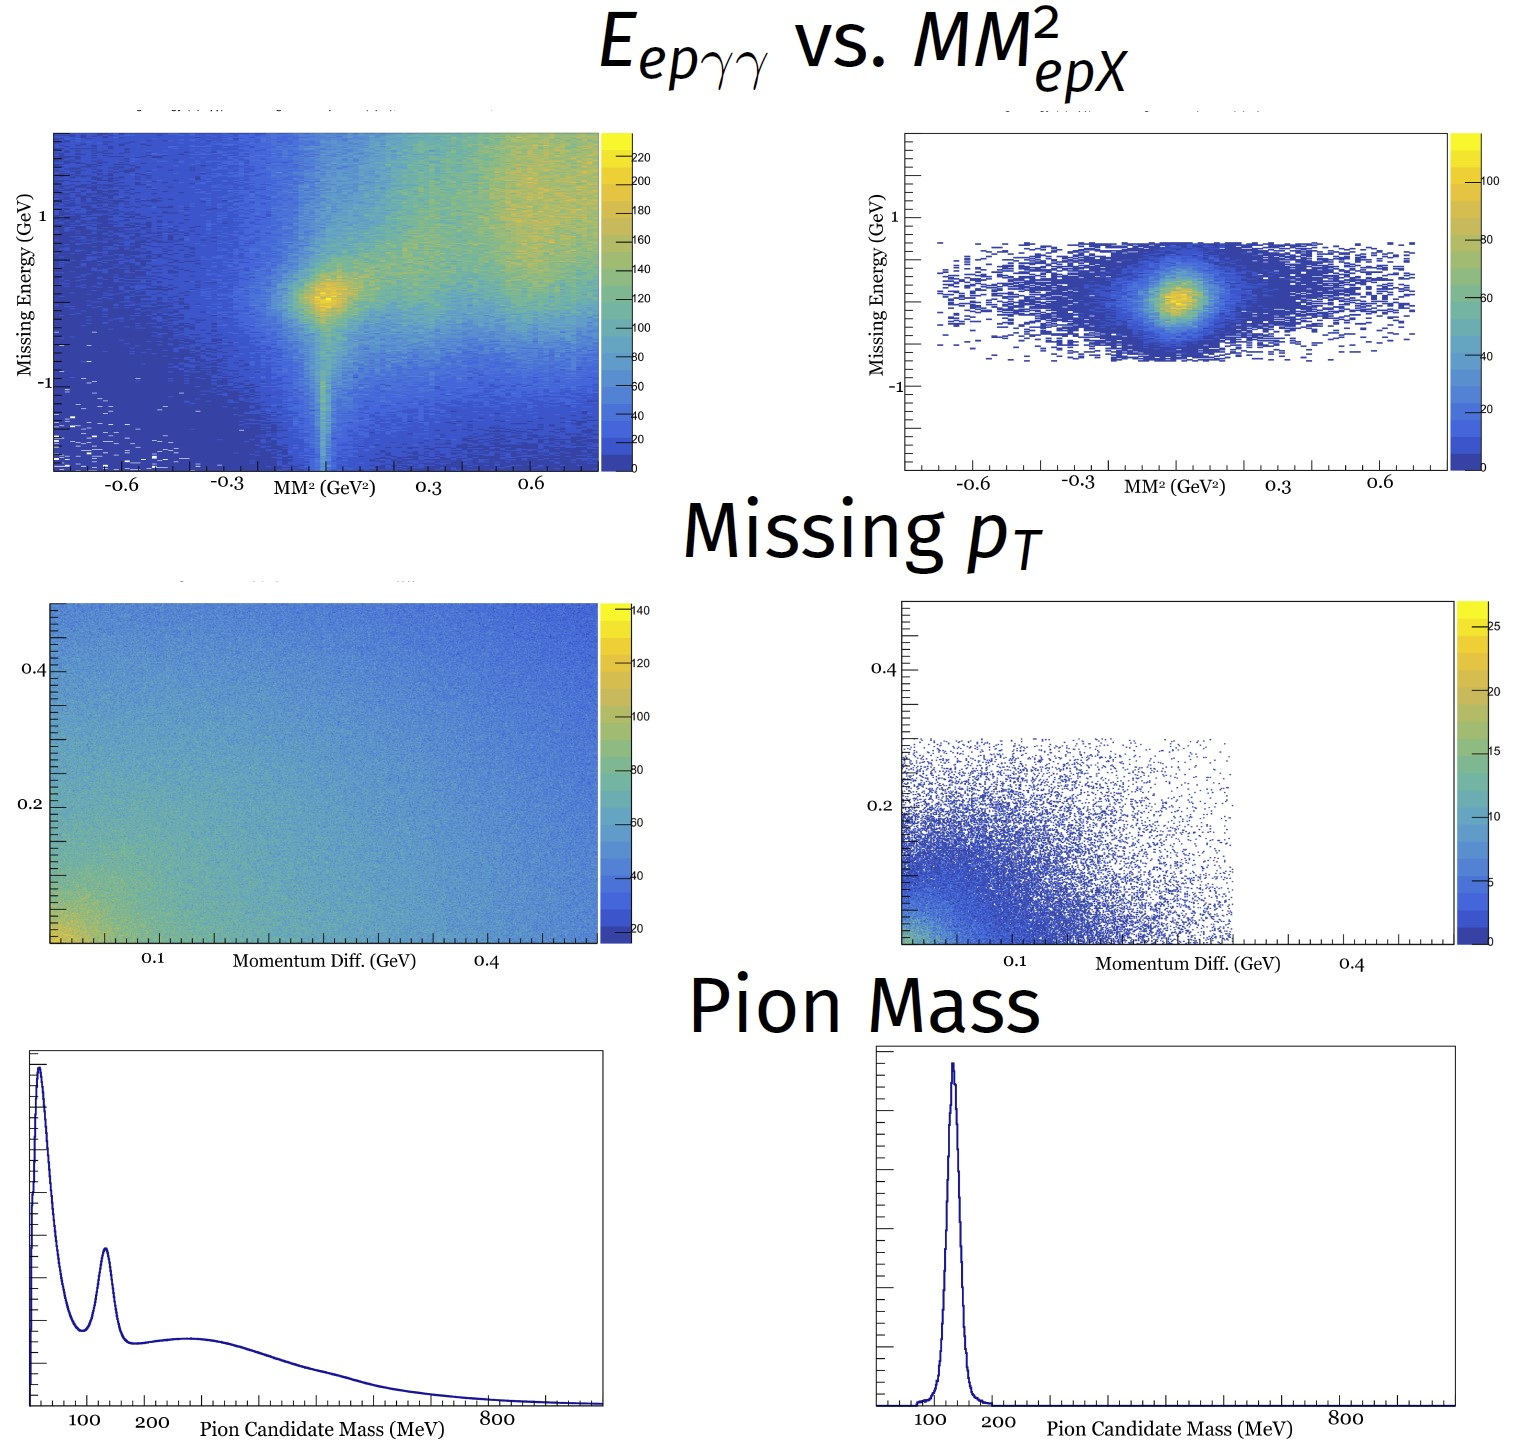
\includegraphics[trim={0 0  0 0cm} ,clip,width=.92\textwidth]{extra/exclusivity.jpg}

                	


        \end{columns}
        \end{column}   
        \end{columns}
\end{frame}


\begin{frame}{Acceptance Correction - Event Generator and Simulation}
     \begin{columns}[c]
               \begin{column}{0.5\textwidth}

                    %\vspace{1cm}
                    \begin{itemize}
                        \item Event Generator - aao\_norad
                            \begin{itemize}
                                \item Nonradiative $DV\pi^0P$ generator validated on CLAS6 and COMPASS data
                            \end{itemize}
                        \item Simulation - GEMC
                            \begin{itemize}
                                \item GEANT4 based simulation developed by CLAS collaboration
                            \end{itemize}
                        \item Computing Power
                            \begin{itemize}
                                \item Through OSG pipeline, CLAS has access to supercomputing clusters around the world, including dedicated nodes at MIT Tier 2, UConn, INFN, GRIDPP, and more
                            \end{itemize}
                    \end{itemize}
                    \end{column}
                    
                    
    \begin{column}{0.5\textwidth}
                
                \centering Generated \\
        \begin{columns}
                    
                    \column{0.5\textwidth}
                        %\textcolor{white}{blank space}
                             
                    
                            %#---------------------------------------------
                           	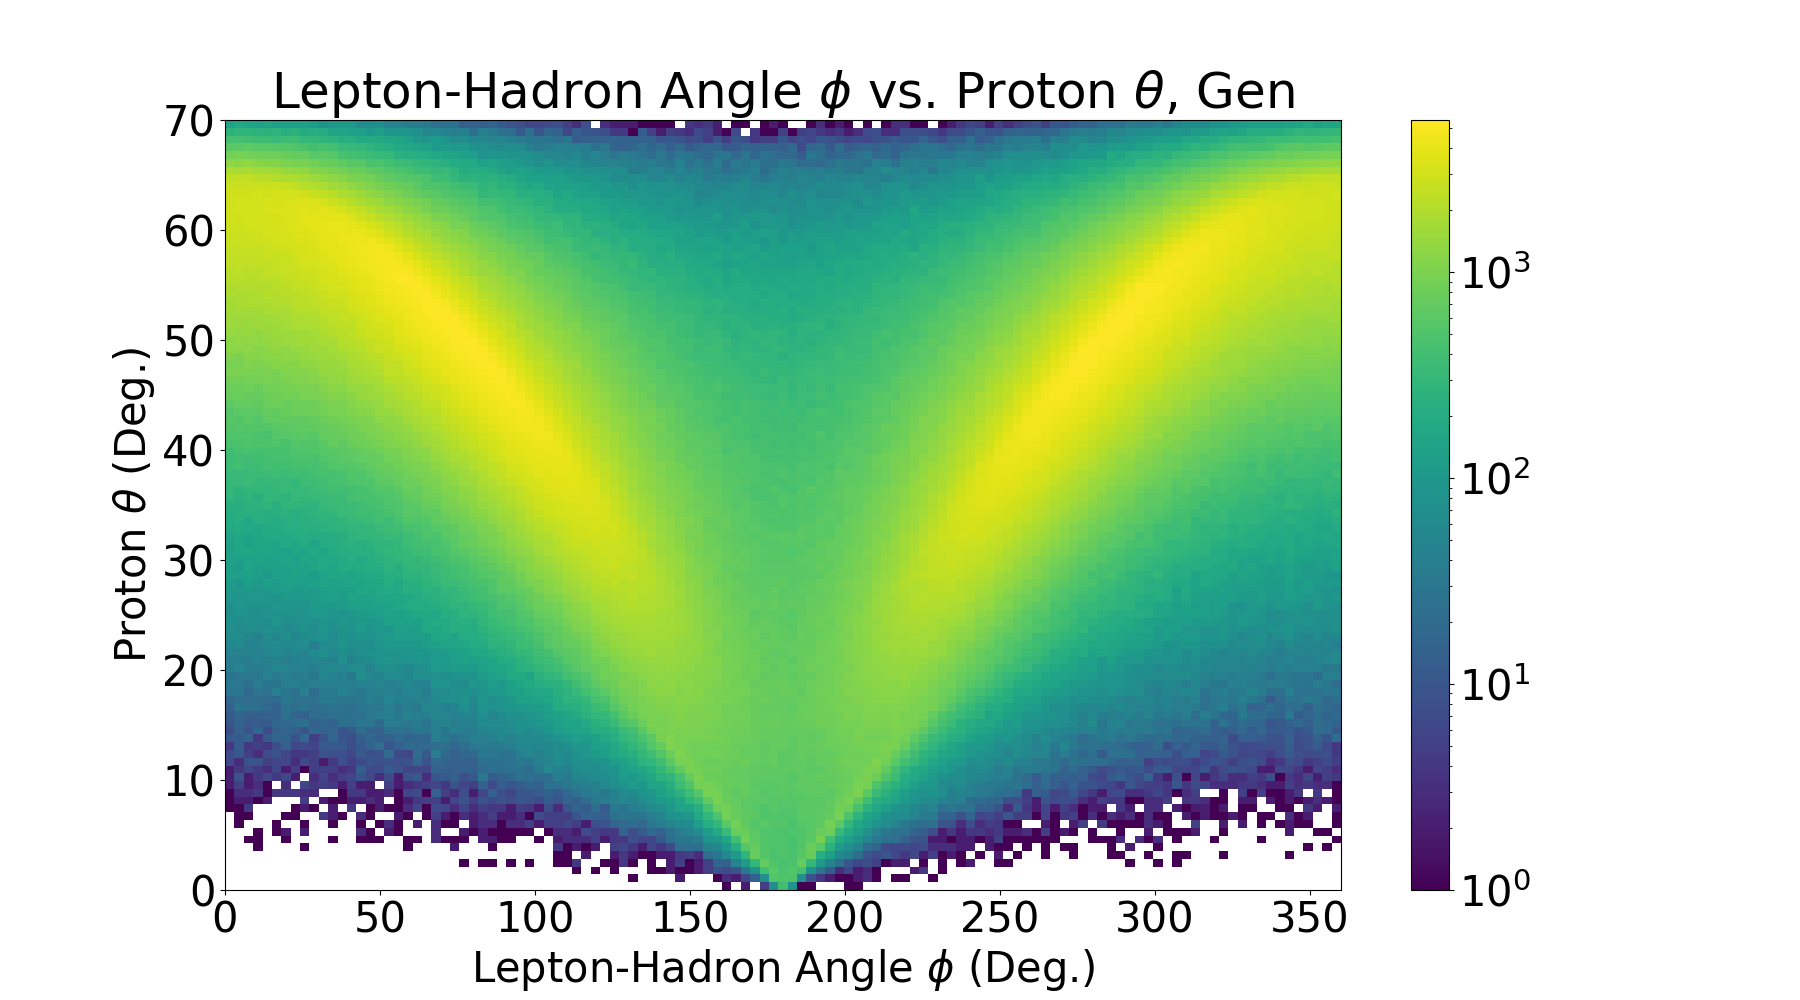
\includegraphics[trim={0 0  0 0cm} ,clip,width=.982\textwidth]{extra/generator/Lepton-Hadron_Angle_phi_vs_Proton_theta,_Gen.png}
                           	   
                  \column{0.5\textwidth}          	   
                           	
                        	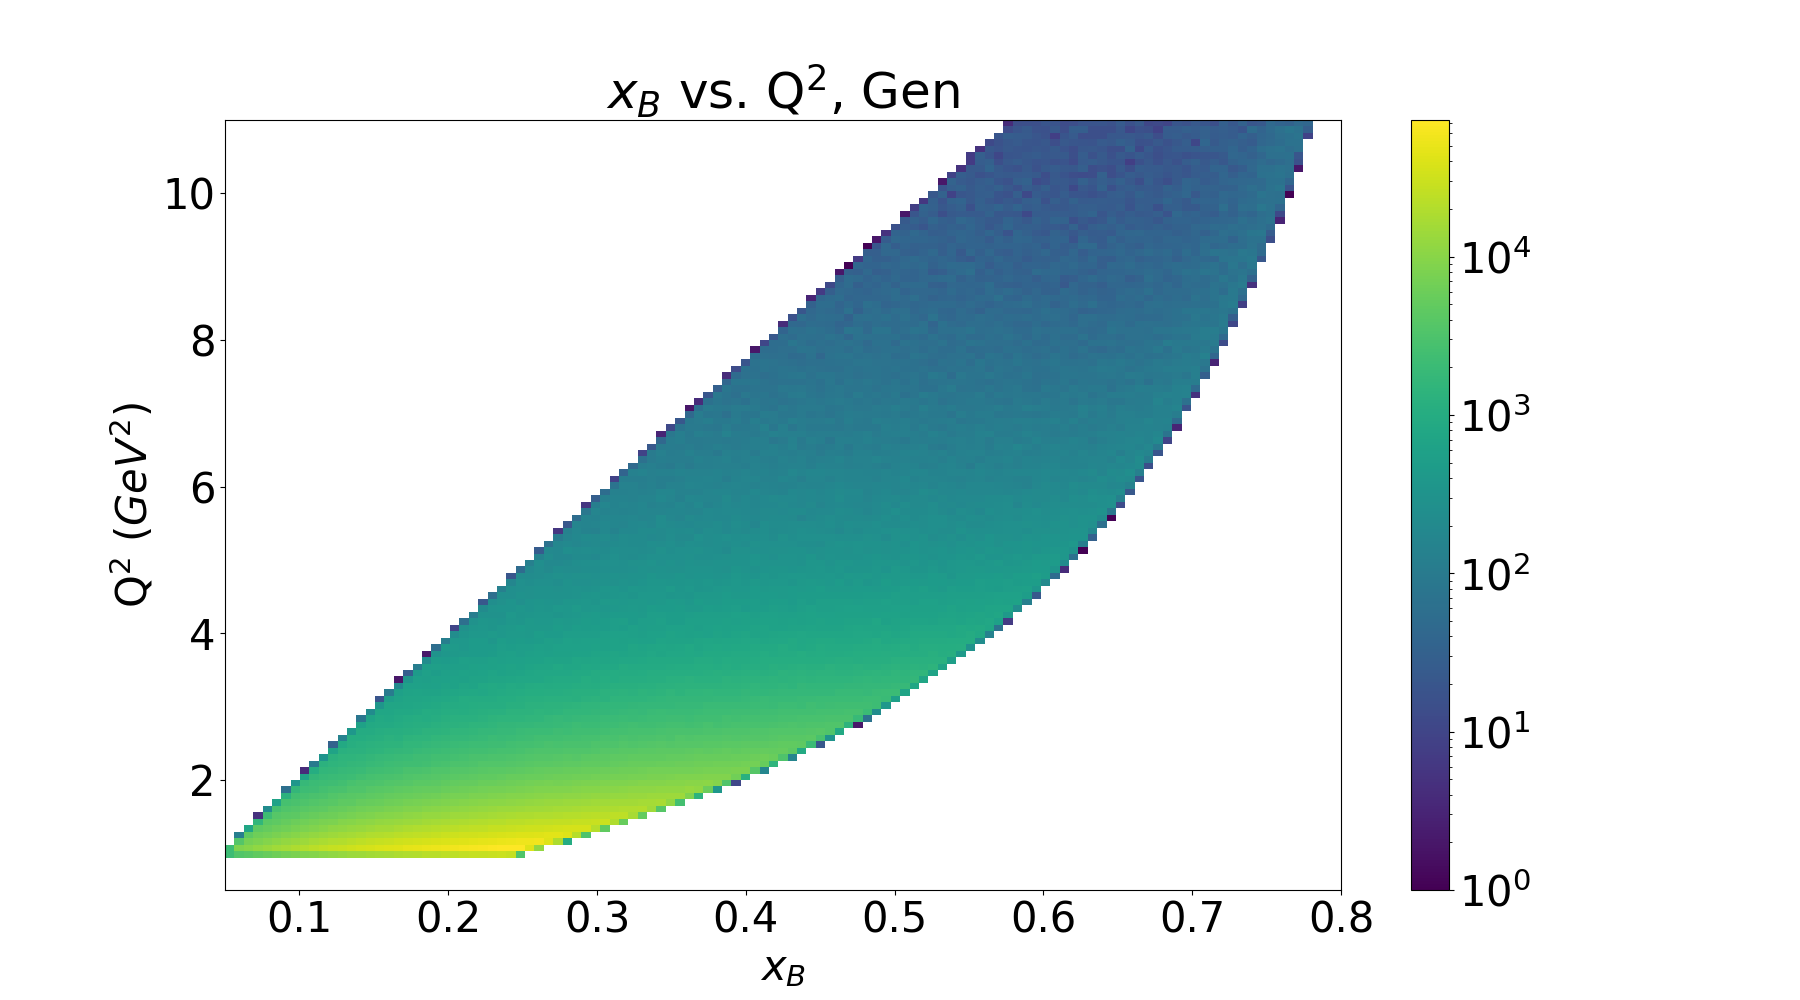
\includegraphics[trim={0 0  0 0cm} ,clip,width=.982\textwidth]{extra/generator/x_B_vs_Q2,_Gen.png}
            
                        \end{columns}
                        \vspace{0.3cm}
              \centering Reconstructed \\      
          \begin{columns} 
            
            
                        \column{0.5\textwidth}
             
                               
                           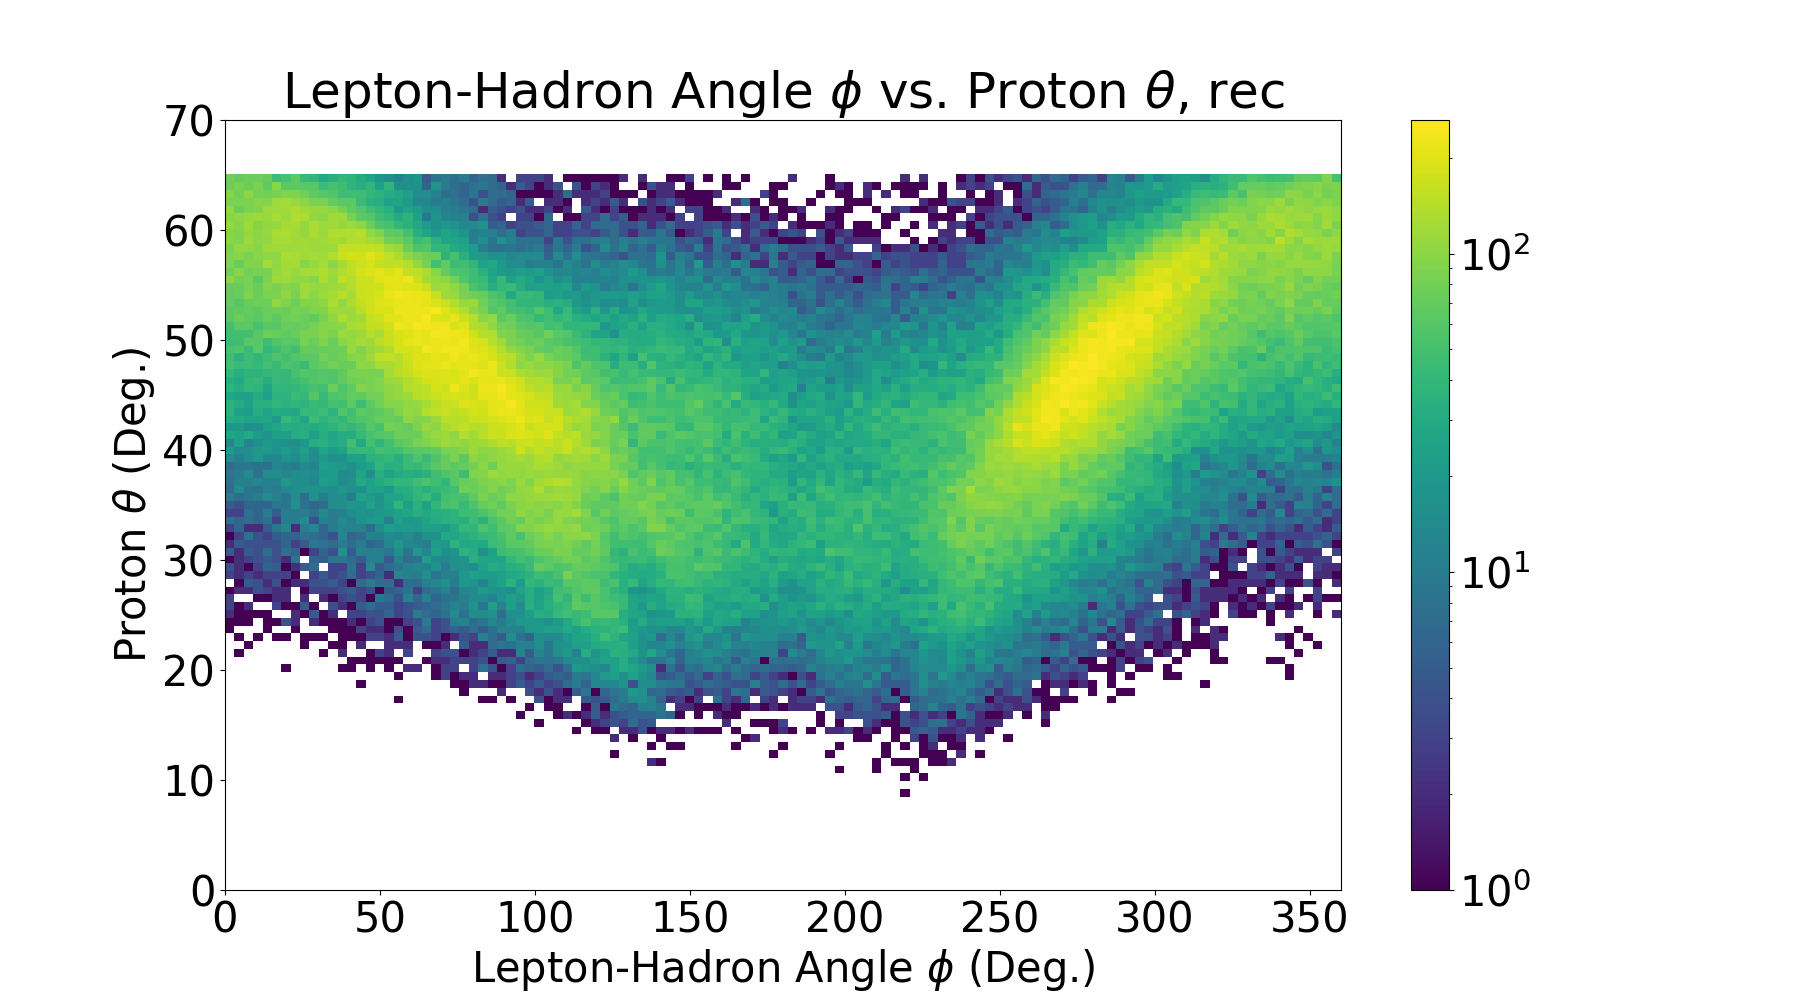
\includegraphics[trim={0 0  0 0cm} ,clip,width=.982\textwidth]{extra/generator/Lepton-Hadron_Angle_phi_vs_Proton_theta,_rec.png}
           \column{0.5\textwidth}
                              
                        	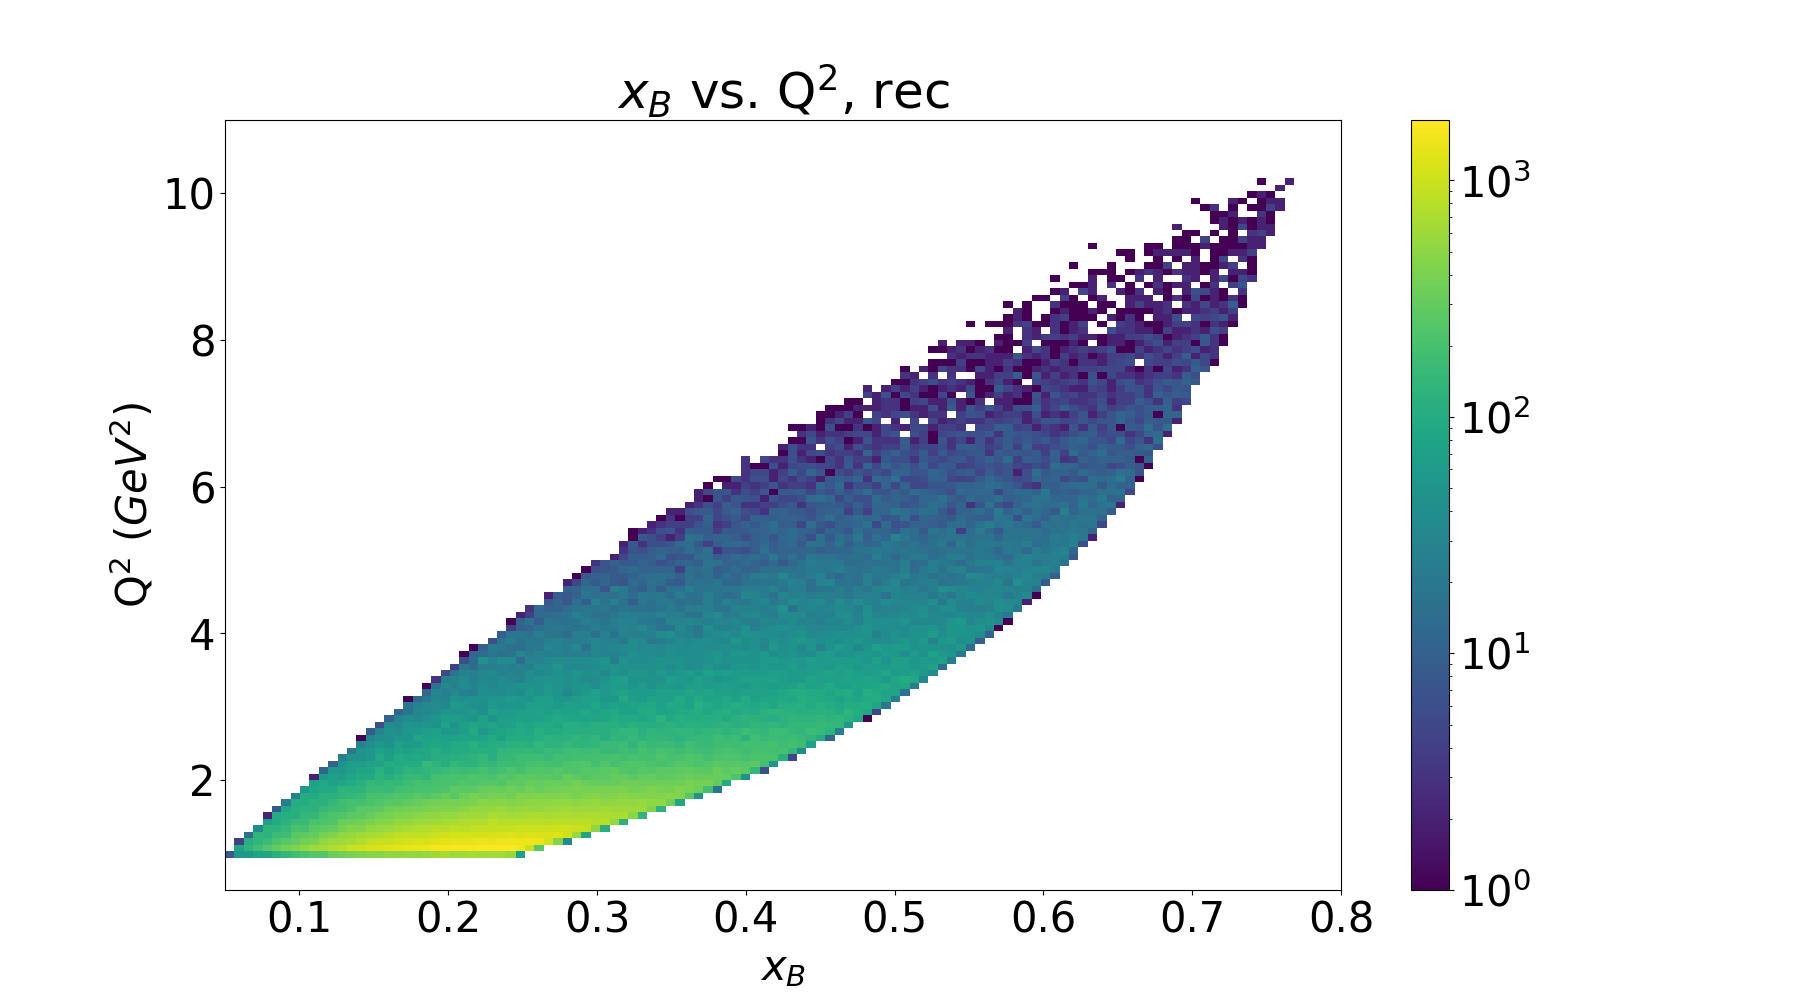
\includegraphics[trim={0 0  0 0cm} ,clip,width=.982\textwidth]{extra/generator/x_B_vs_Q2,_rec.png}
        
                \end{columns}
    \end{column}
                    
    \end{columns}
\end{frame}

\begin{frame}{Acceptance Correction - Simulation : Experiment Matching}

With the addition of smearing factors to simulated particle reconstruction values, the simulation matches experimental distributions well.  {\myfont{\footnotesize [Collaborator S. Lee]}}




\vspace{0.2cm}
\begin{columns}
            \column{0.32\textwidth}
                %\textcolor{white}{blank space}
                     \centering $ME_{ep\gamma\gamma}$ \\
                        % trim={<left> <lower> <right> <upper>}
                    %#---------------------------------------------
                   	\includegraphics[trim={0 1.75cm  0 3.05cm} ,clip,width=.82\textwidth]{simcomp/yessmear/outbending_rad_All_All_All_for_aps_2022_plots_sangcutsME_epgg_exp_vs_sim.png}
                   	   \centering  $MM^2_{e\gamma\gamma}$ \\
                	\includegraphics[trim={0 1.75cm  0 3.05cm} ,clip,width=.82\textwidth]{simcomp/yessmear/outbending_rad_All_All_All_for_aps_2022_plots_sangcutsMM2_egg_exp_vs_sim.png}


                \column{0.32\textwidth}
     
                       \centering  $MM^2_{ep\gamma\gamma}$ \\
                	\includegraphics[trim={0 1.75cm  0 3.05cm} ,clip,width=.82\textwidth]{simcomp/yessmear/outbending_rad_All_All_All_for_aps_2022_plots_sangcutsMM2_epgg_exp_vs_sim.png}
   
                      \centering   $MM^2_{ep}$ \\
                	\includegraphics[trim={0 1.75cm  0 3.05cm} ,clip,width=.82\textwidth]{simcomp/yessmear/outbending_rad_All_All_All_for_aps_2022_plots_sangcutsMM2_ep_exp_vs_sim.png}

            
            \column{0.32\textwidth}

                    %#---------------------------------------------
                      \centering   $M_{\gamma\gamma}$ \\
                	\includegraphics[trim={0 1.75cm  0 3.05cm} ,clip,width=.82\textwidth]{simcomp/yessmear/outbending_rad_All_All_All_for_aps_2022_plots_sangcutsMpi0_exp_vs_sim.png}
 
                       \centering  $\Delta p_{t}$ \\
                	\includegraphics[trim={0 1.75cm  0 3.05cm} ,clip,width=.82\textwidth]{simcomp/yessmear/outbending_rad_All_All_All_for_aps_2022_plots_sangcutsMPt_exp_vs_sim.png}

    \end{columns}
\end{frame} 

\begin{frame}{Progress on Preliminary Cross Section}

\begin{columns}
\column{0.4\textwidth}

    \begin{itemize}
        \item Acceptance corrected data follows functional form expected from structure function decomposition
                        
    \end{itemize}



            \column{0.3\textwidth}
                %\textcolor{white}{blank space}
                    
            
                    %#---------------------------------------------
                   	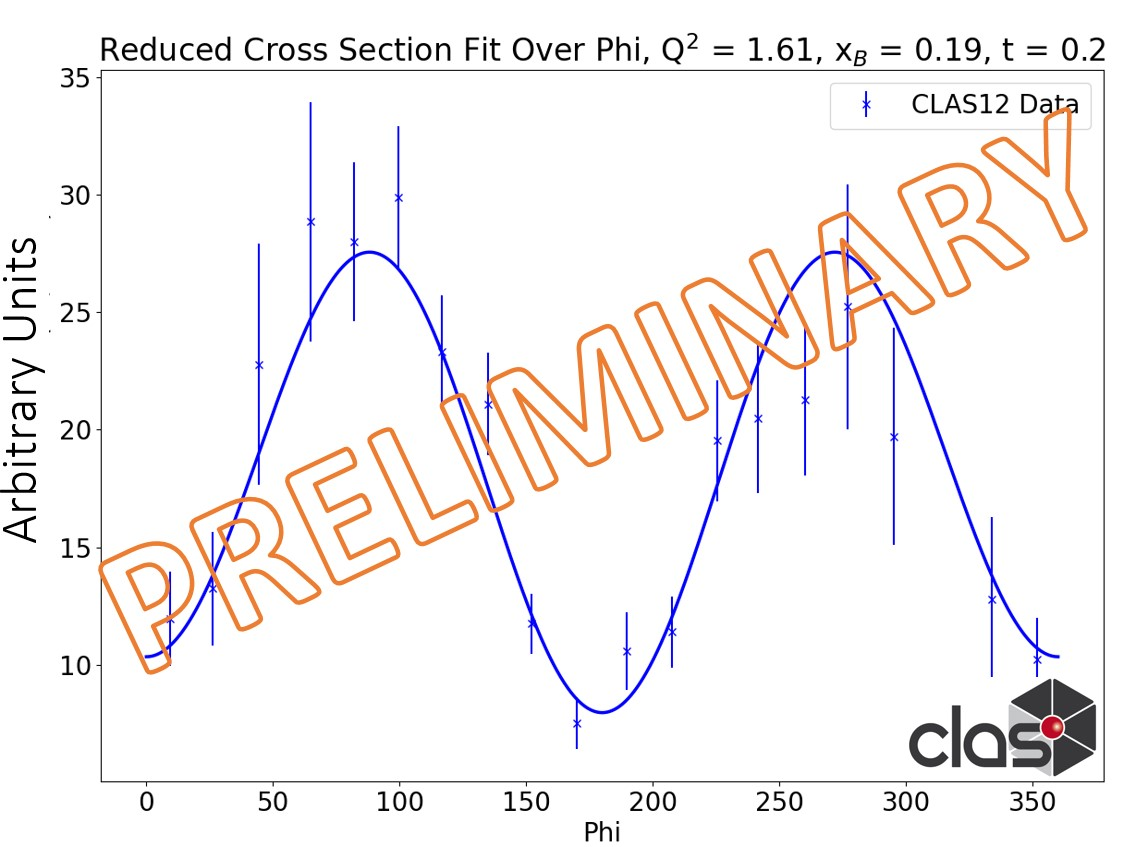
\includegraphics[trim={0 0  0 0cm} ,clip,width=.882\textwidth]{extra/xsec/fit1.jpg}
                   	\vspace*{-1.1cm}  % Tune this to the image height.
                    \begin{center}
                    \scalebox{.4}{\color{gray}*Err. bars stat. only          }
                    \end{center}
                    \vspace*{.2cm} 
                   	  
                	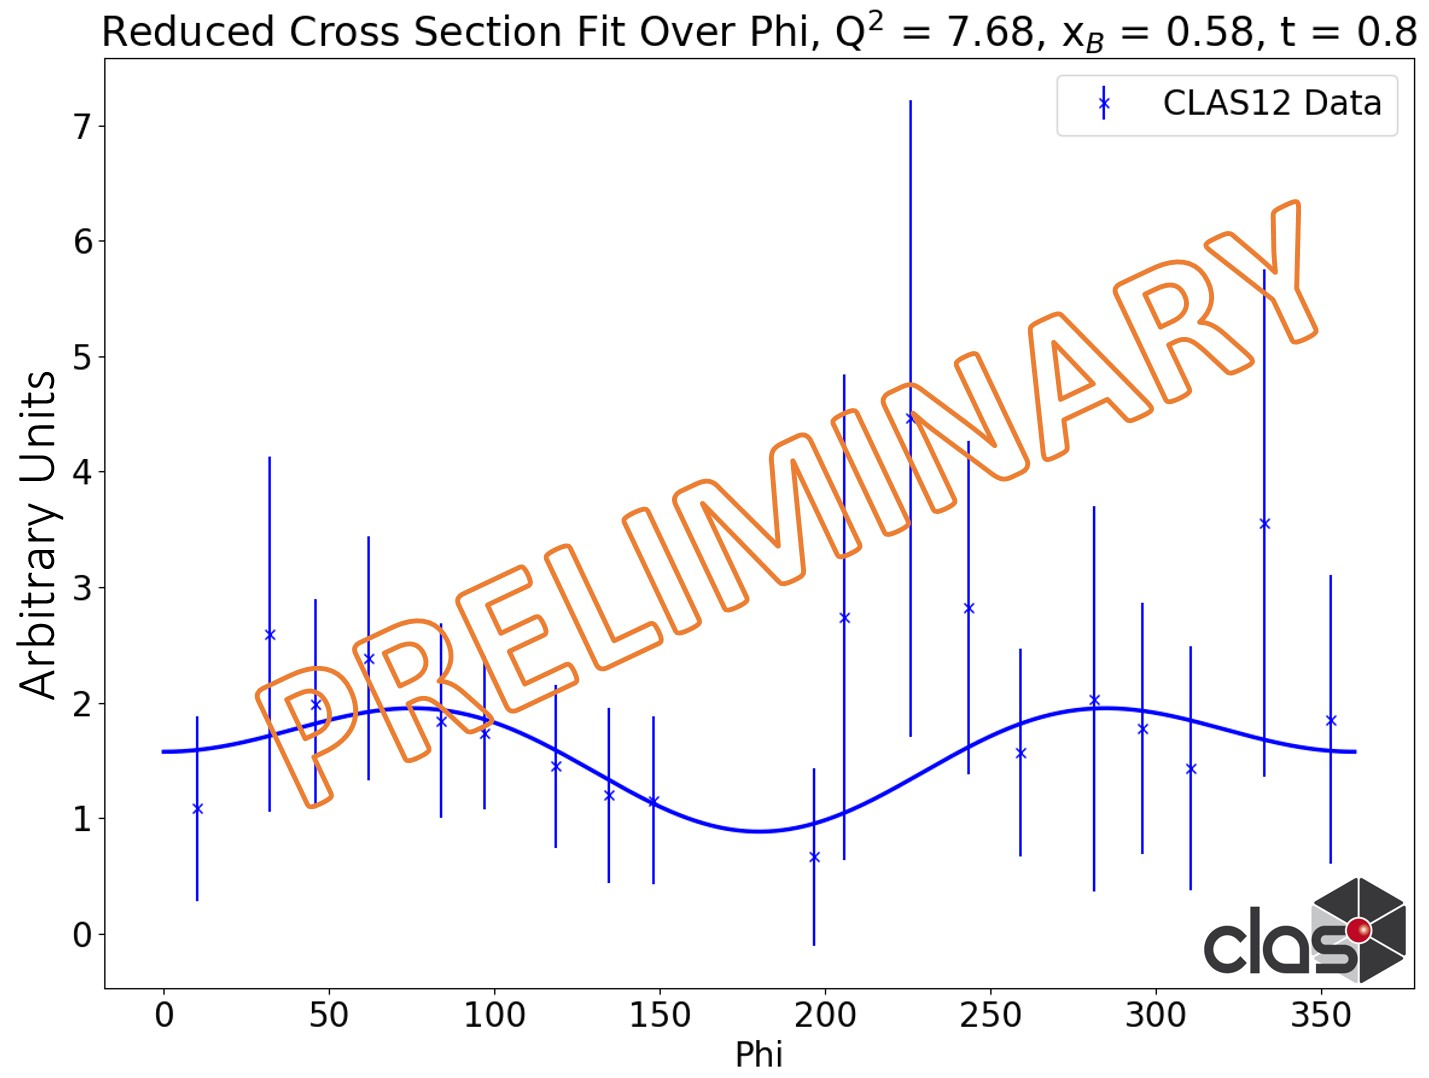
\includegraphics[trim={0 0  0 0cm} ,clip,width=.882\textwidth]{extra/xsec/xsec_7.jpg}
                	                   	\vspace*{-1.1cm}  % Tune this to the image height.
                    \begin{center}
                    \scalebox{.4}{\color{gray}*Err. bars stat. only          }
                    \end{center}
                    \vspace*{.2cm} 
       
                   \column{0.3\textwidth}
                %\textcolor{white}{blank space}
                     
            
                    %#---------------------------------------------
                   	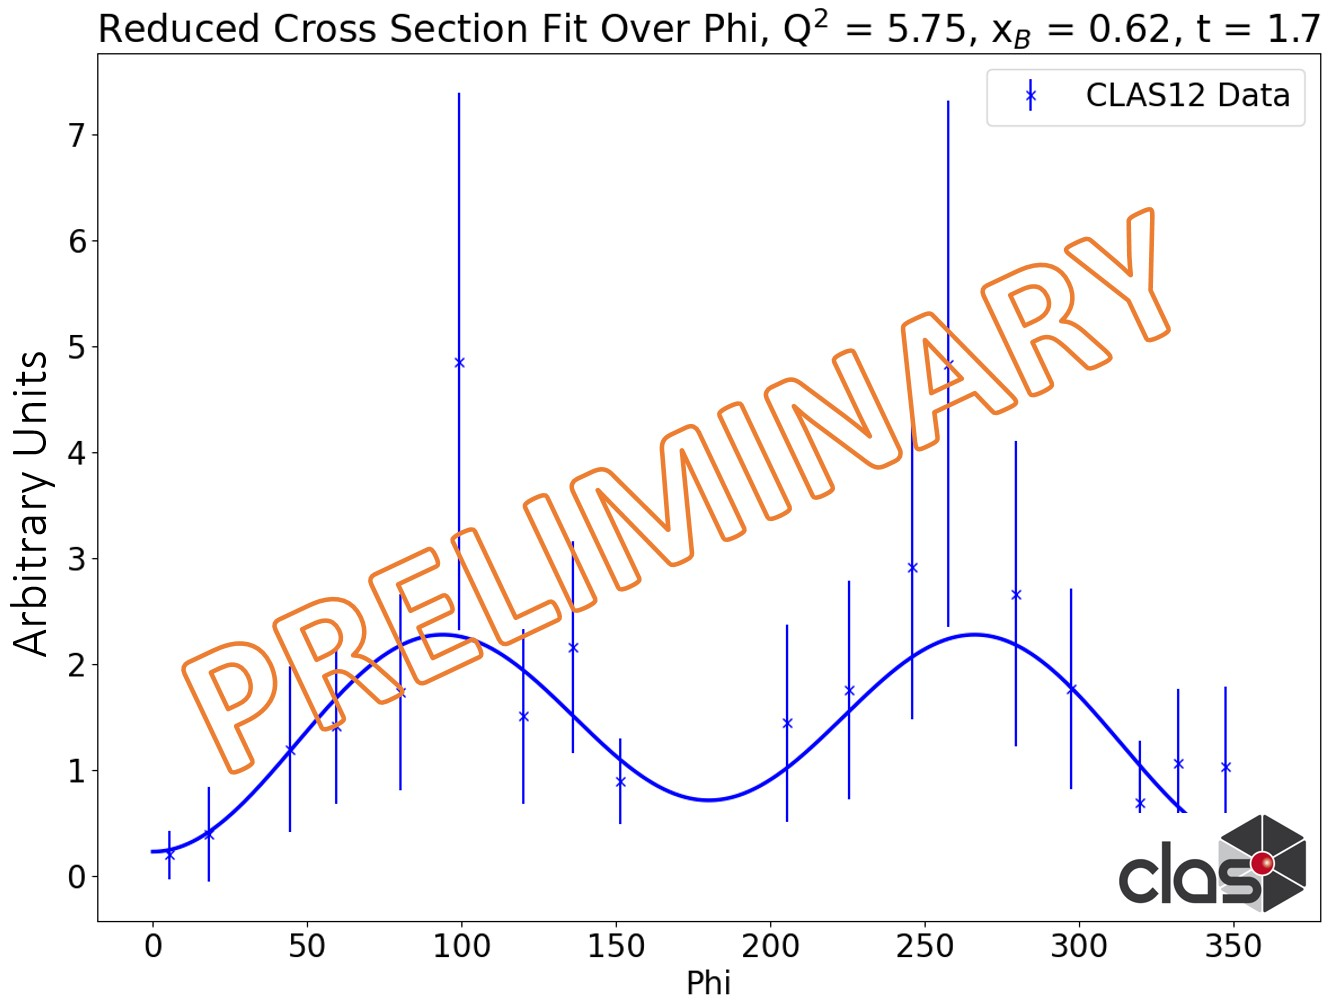
\includegraphics[trim={0 0  0 0cm} ,clip,width=.882\textwidth]{extra/xsec/xsec_5.jpg}
                   	                      	\vspace*{-1.1cm}  % Tune this to the image height.
                    \begin{center}
                    \scalebox{.4}{\color{gray}*Err. bars stat. only          }
                    \end{center}
                    \vspace*{.2cm} 
                    
                	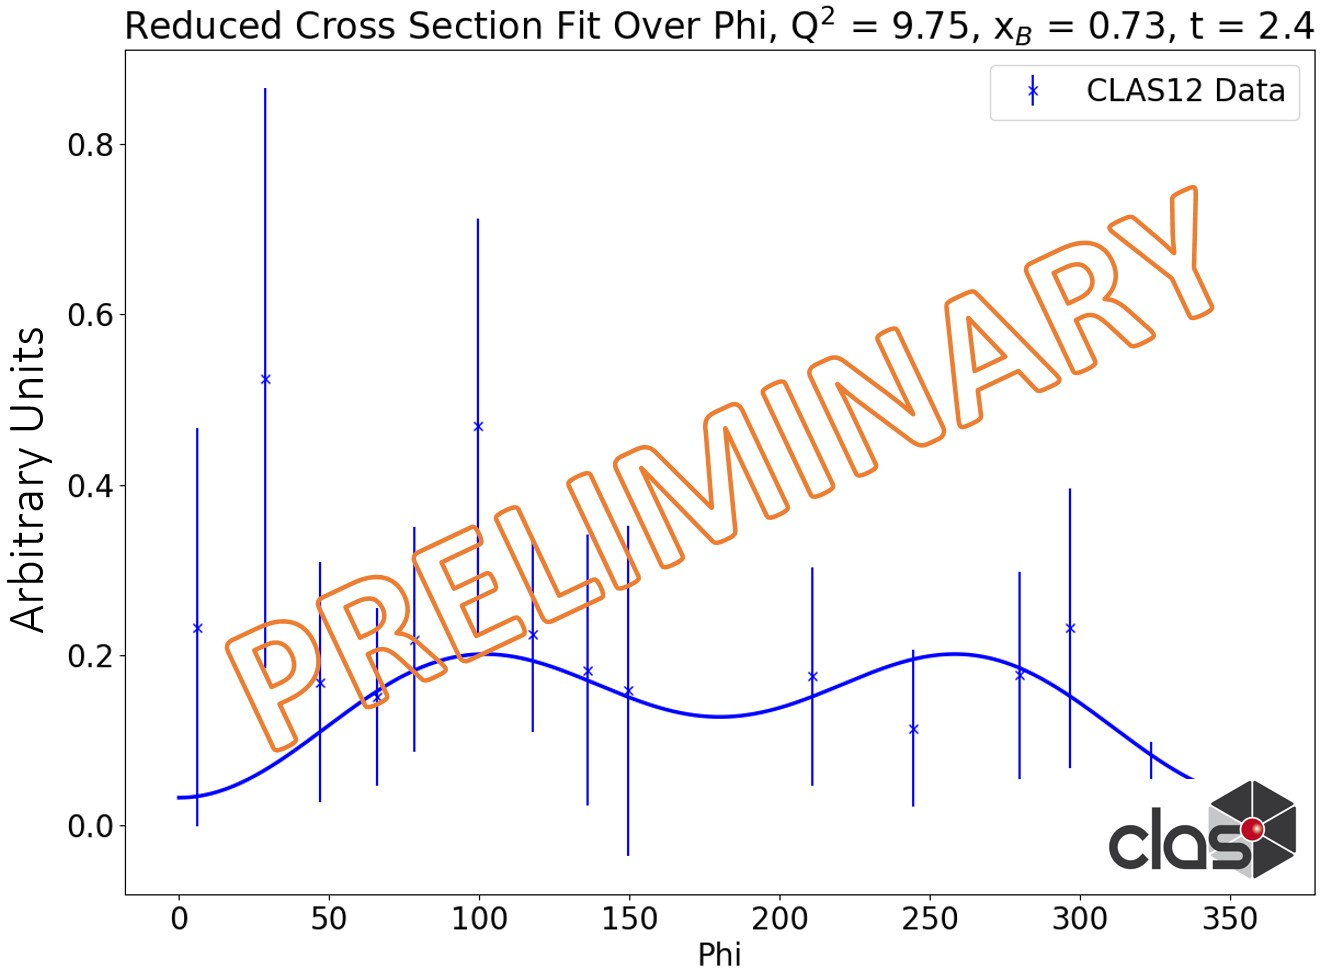
\includegraphics[trim={0 0  0 0cm} ,clip,width=.882\textwidth]{extra/xsec/xsec_9.jpg}
                	                   	\vspace*{-1.1cm}  % Tune this to the image height.
                    \begin{center}
                    \scalebox{.4}{\color{gray}*Err. bars stat. only          }
                    \end{center}
                    \vspace*{.2cm} 
       
       
       \end{columns}         	

\end{frame}



\begin{frame}{Theory Predictions - GK Model}
\begin{columns}[t, onlytextwidth]
            \column{0.4\textwidth}
            
                \begin{itemize}
                    \setlength\itemsep{1em}
                    \item \footnotesize Goloskokov-Kroll (GK) model predicts exclusive $\pi$ electroproduction cross sections using handbag approach\\
                    {\myfont{\tiny [S.V. Goloskokov $\&$ P. Kroll, EPJC, 65,137 (2010)]}}

                    \item Model parameters chosen to best describe recent CLAS $\pi^+$ BSA result\\
                    {\myfont{\tiny [S. Diehl et al., PRL 125 182001 (2020)]}}
                    
                    \item Software implementation from\\
                    K. Tezgin / PARTONS Framework\\
                    {\myfont{\tiny [B. Berthou et al., EPJC, 78, 478 (2018)]}}
                    
                    \end{itemize}
                    
                    \vspace{0.1cm}
                    \footnotesize Note: 
                    \vspace{0.1cm}
                     
                     \scalebox{0.835}{
                        W $>$ 2 GeV $\implies \frac{Q^2\left( 1-x_B\right)}{x_B} > 3.12$ GeV$^2$
                        }\\
                     
                     \scalebox{0.835}{
                            $t > t_{min} \implies t> \frac{m_p^2x_B^2}{1-x_B}$
                     }
                
                
            \column{0.3\textwidth}
            \centering
                Model Predictions\\
                	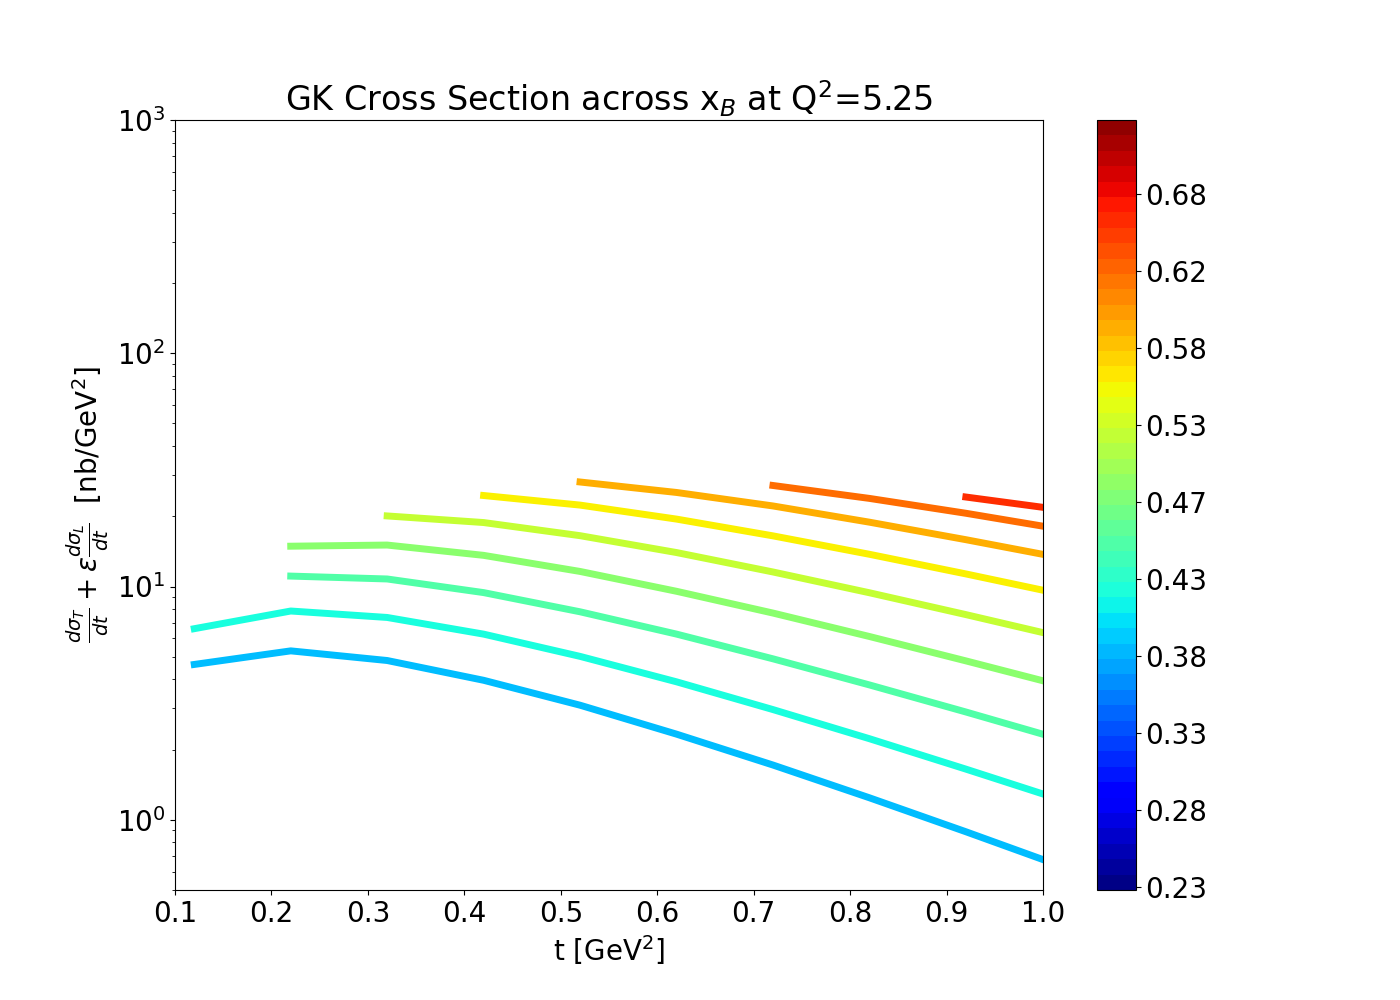
\includegraphics[trim={0 0  0 0cm} ,clip,width=.9882\textwidth]{DNP/gk_q2/fig_8_q2_5.25.png}
                	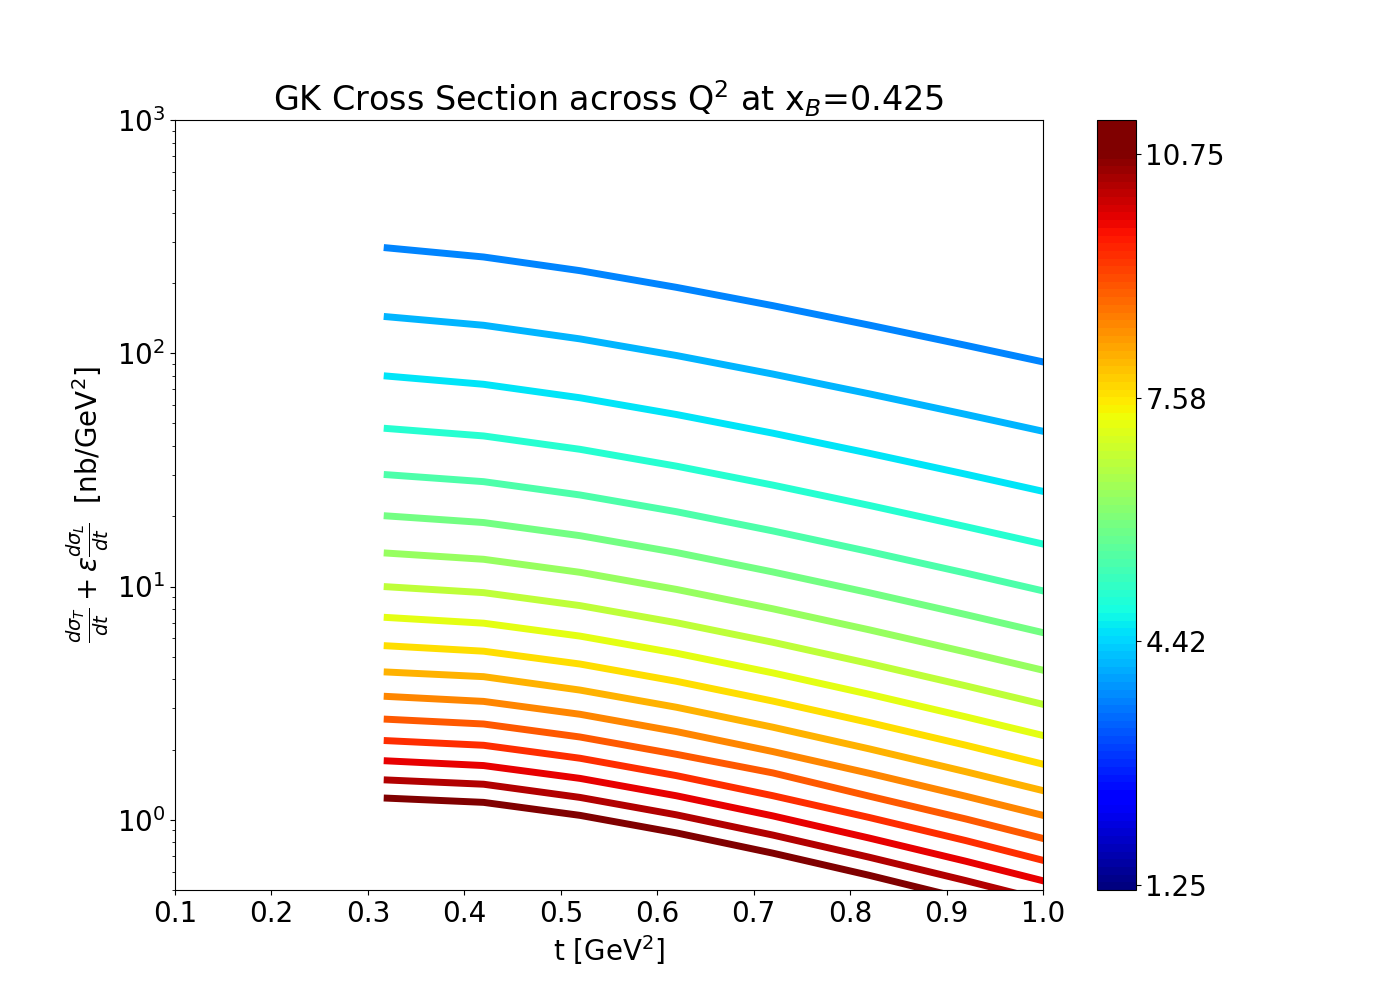
\includegraphics[trim={0 0  0 0cm} ,clip,width=.9882\textwidth]{DNP/gk_xb/fig_4_xb_0.425.png}
                		
            \column{0.3\textwidth}
                \centering
                \vspace{0.2cm}
                GK and CLAS12 Data
                    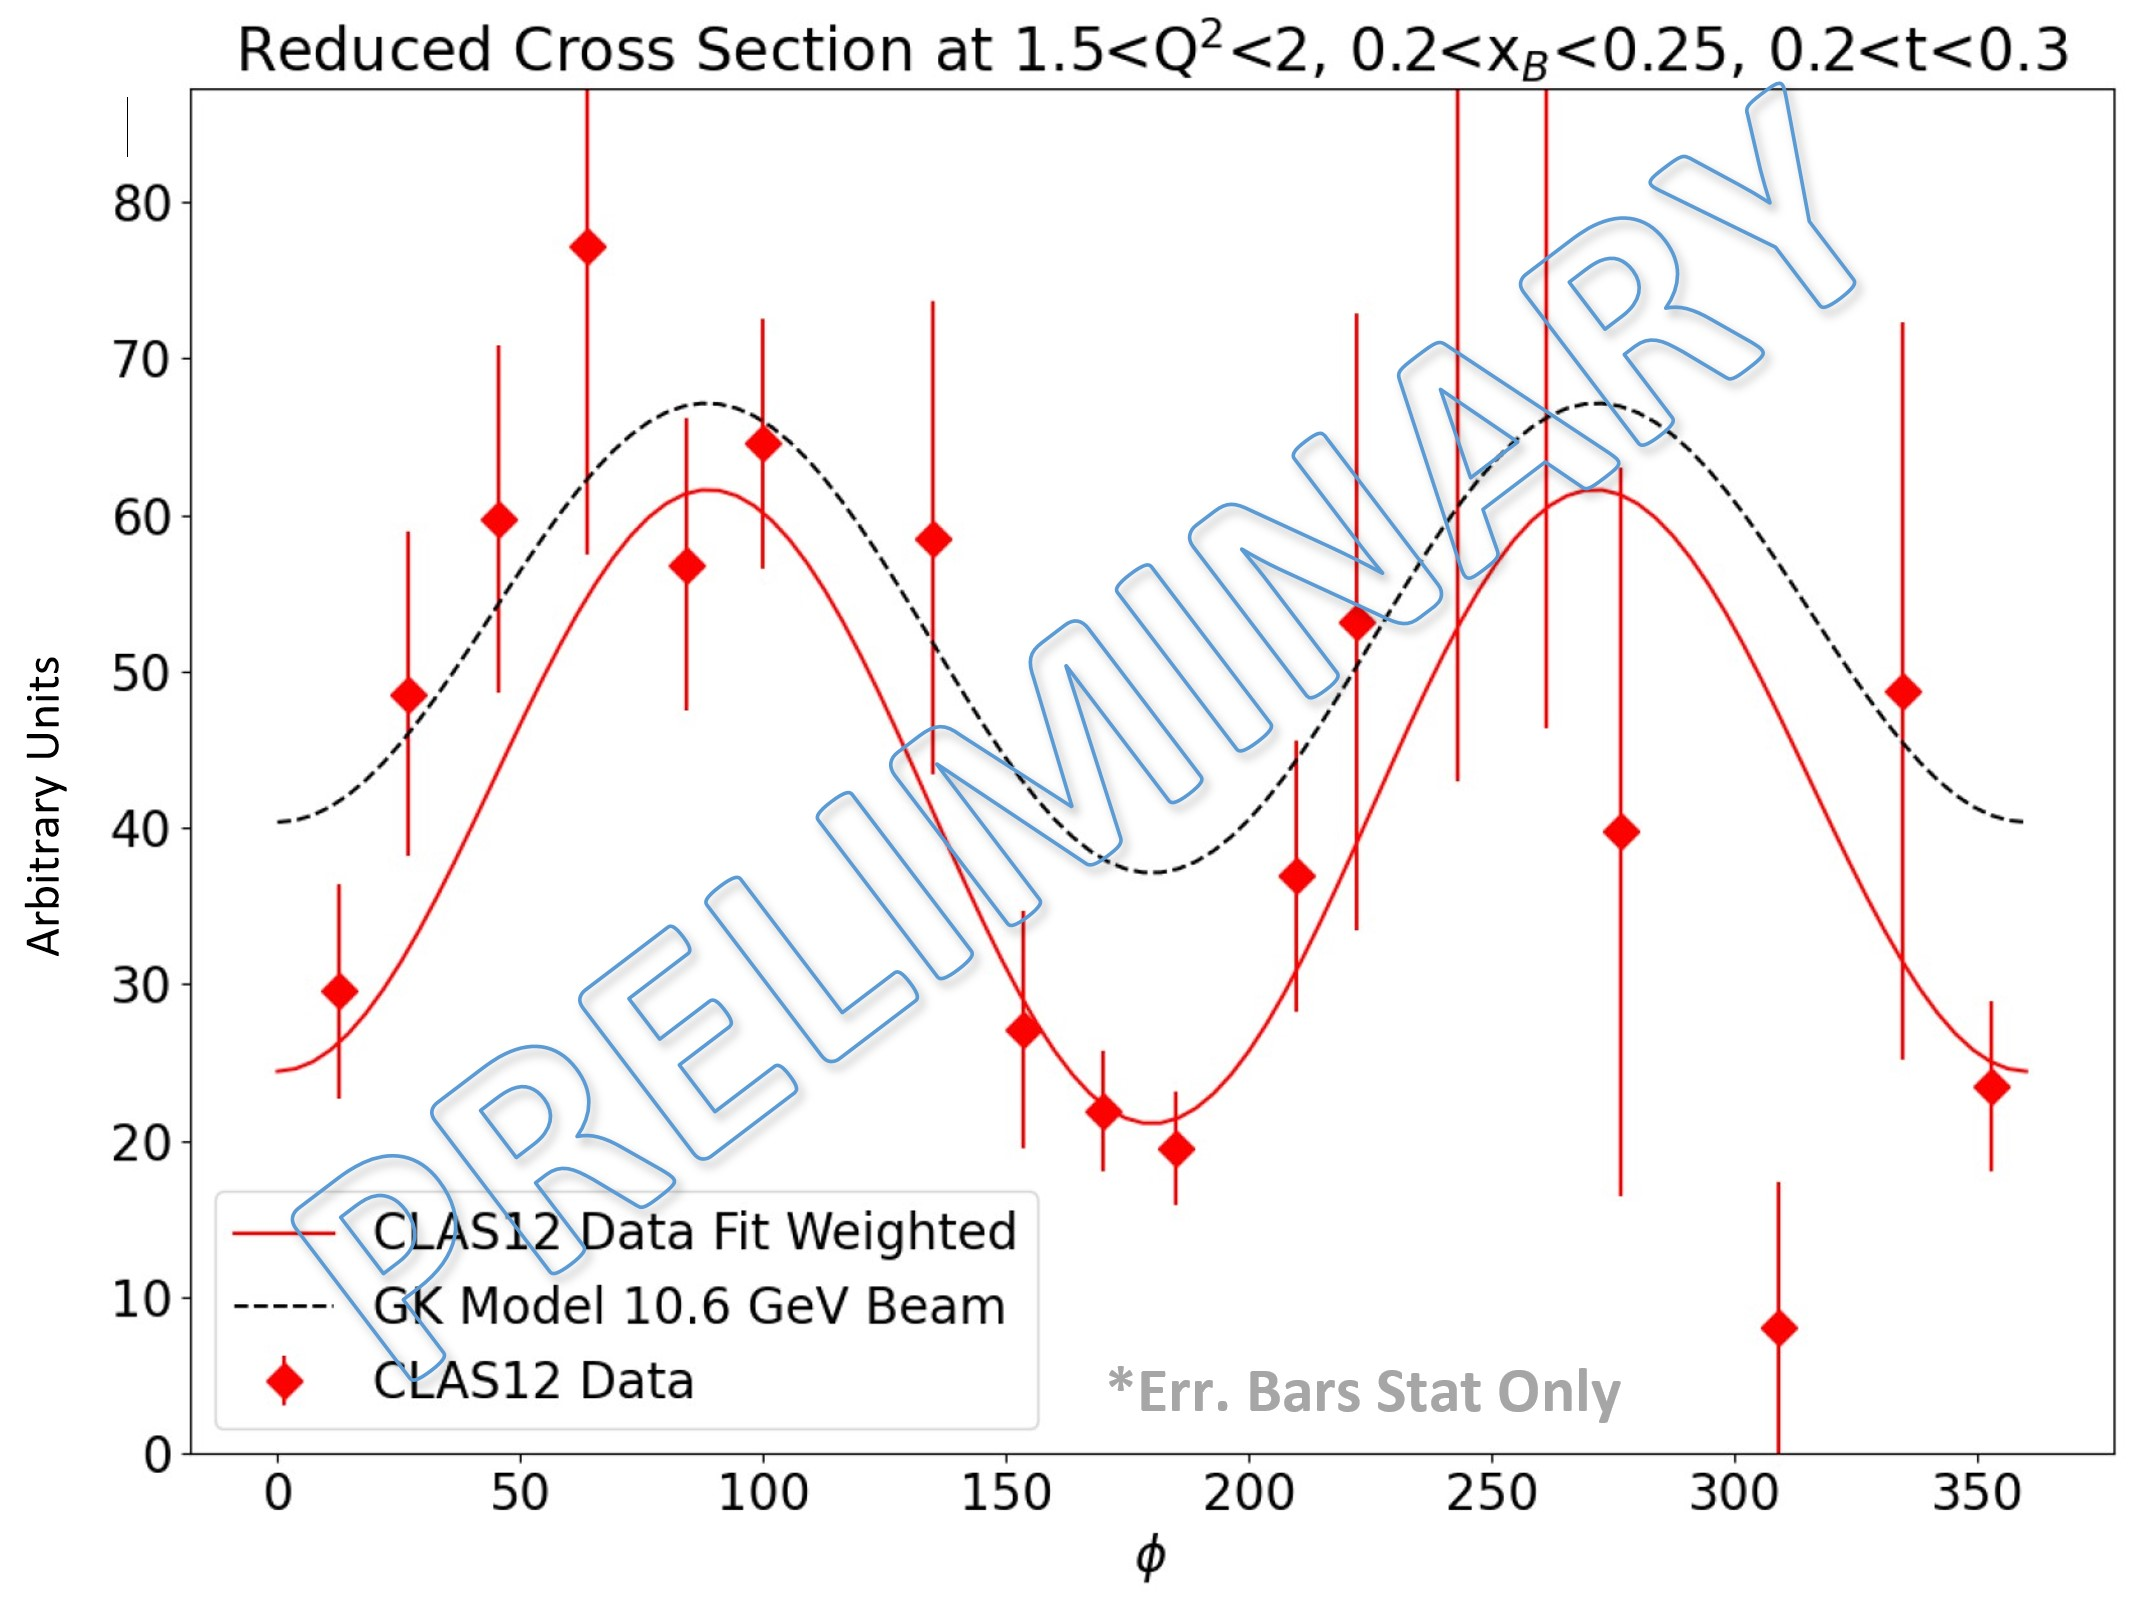
\includegraphics[trim={0 0  0 0cm} ,clip,width=.92\textwidth]{DNP/gk_1.jpg}
                    \vspace{0.1cm}
                	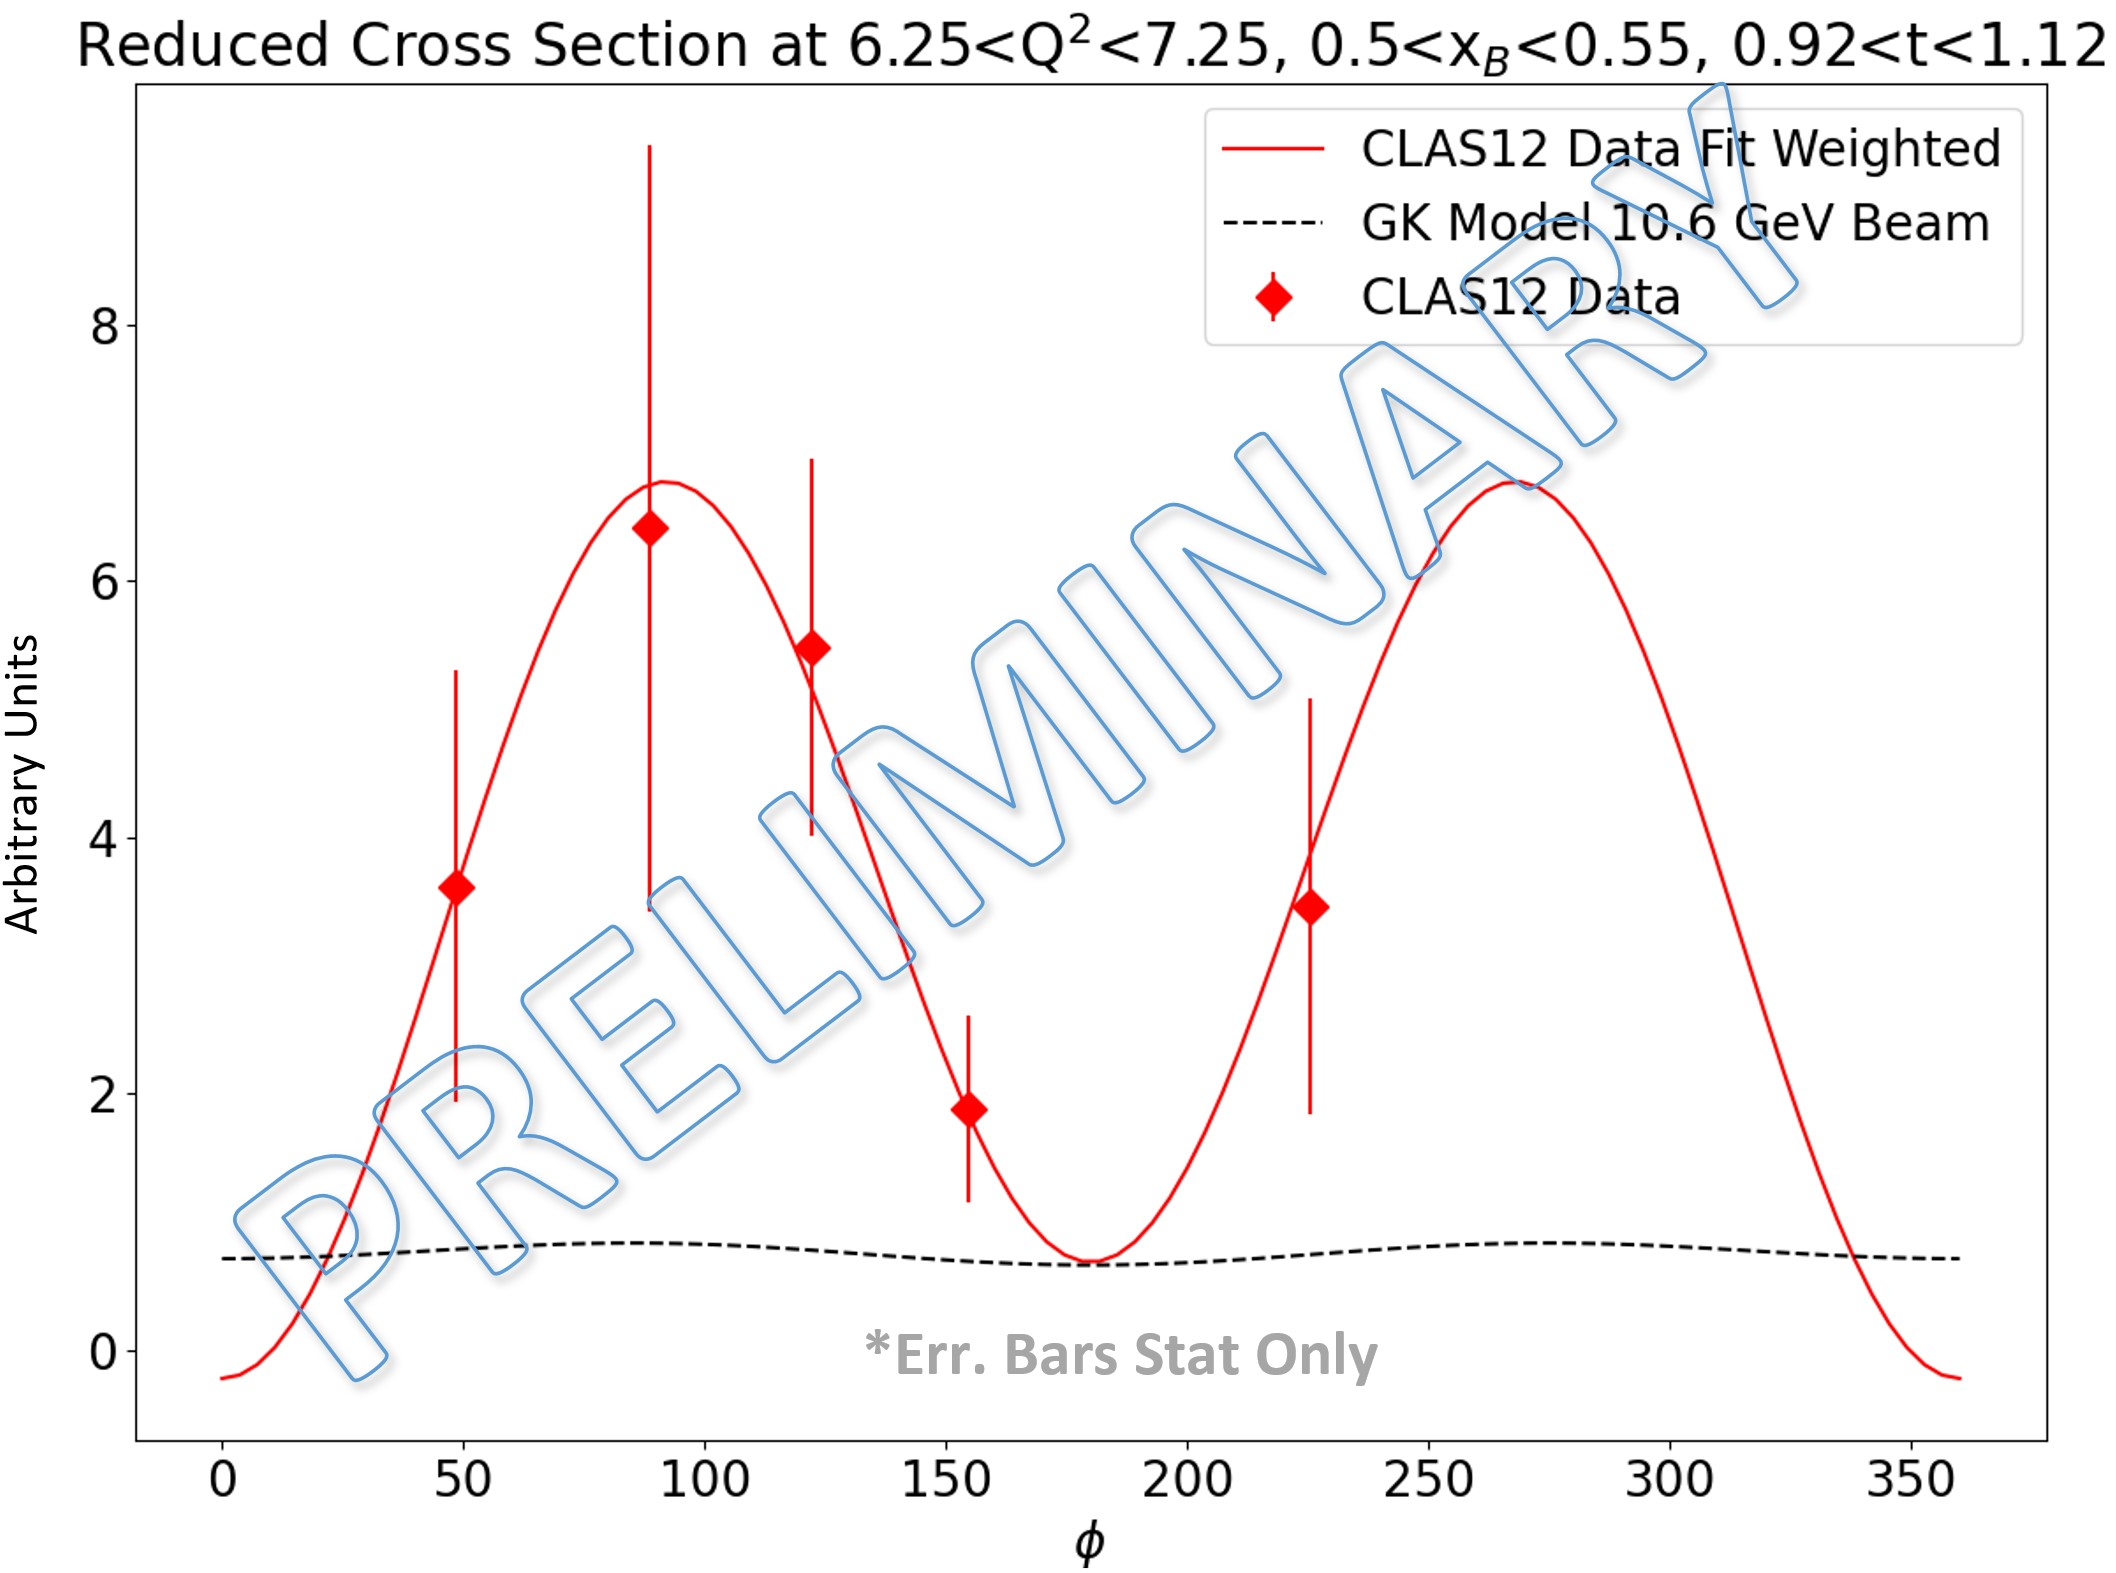
\includegraphics[trim={0 0  0 0cm} ,clip,width=.92\textwidth]{DNP/gk_2.jpg}
                		
                
        \end{columns}
\end{frame}



\begin{frame}{Conclusion - Towards a Full Cross Section}
Preliminary efforts on event selection, simulations, and acceptance corrections yield promising results but more work is needed to extract a complete cross section measurement:
\vspace{0.4cm}
\begin{itemize}
    \setlength\itemsep{1em}
    \item Determination of remaining correction factors - radiative, binning, and absolute normalization
    \item Study of systematic uncertainties 
    \item Quantitative comparisons between data and theory model will be meaningful when uncertainties and binning are more complete
\end{itemize}
    
%Acknowledge: MIT group, Sangbaek Lee, Andrey Kim, CLAS collaboration
\end{frame}



\appendix



\begin{frame}{Finite Bin Volume Corrections}
Bin Average is not the same as bin center


\end{frame}


\begin{frame}{Ditching Binning - OMNIFOLD}
words

\end{frame}

\begin{frame}{Rosenbluth Separation}
Igor Paper

\end{frame}

\begin{frame}{Classifier -- box to manifold}
words

\end{frame}


\begin{frame}{Normalizing Flows}
words

\end{frame}

\begin{frame}{Simulation Based INference}
Words
\end{frame}

\begin{frame}{Extra slides}
Extra Slides

\end{frame}


\begin{frame}{Extra slides}
Extra Slides
Find this on the web at:
https://github.com/robertej19/Thesis-Offense/blob/main/Main/presentation.tex

\end{frame}




\begin{frame}{Backup slides}
      - QCD factorization theorem for DVMP process has only been proven for longitudinally polarized photons\\
    - QCD factorization has been proven for DVCS
 
\end{frame}


\begin{frame}{Acceptance Correction - Bin by Bin Calculation}
\begin{columns}
            \column{0.25\textwidth}
                %\textcolor{white}{blank space}
                     \centering Raw Counts \\
            
                    %#---------------------------------------------
                   	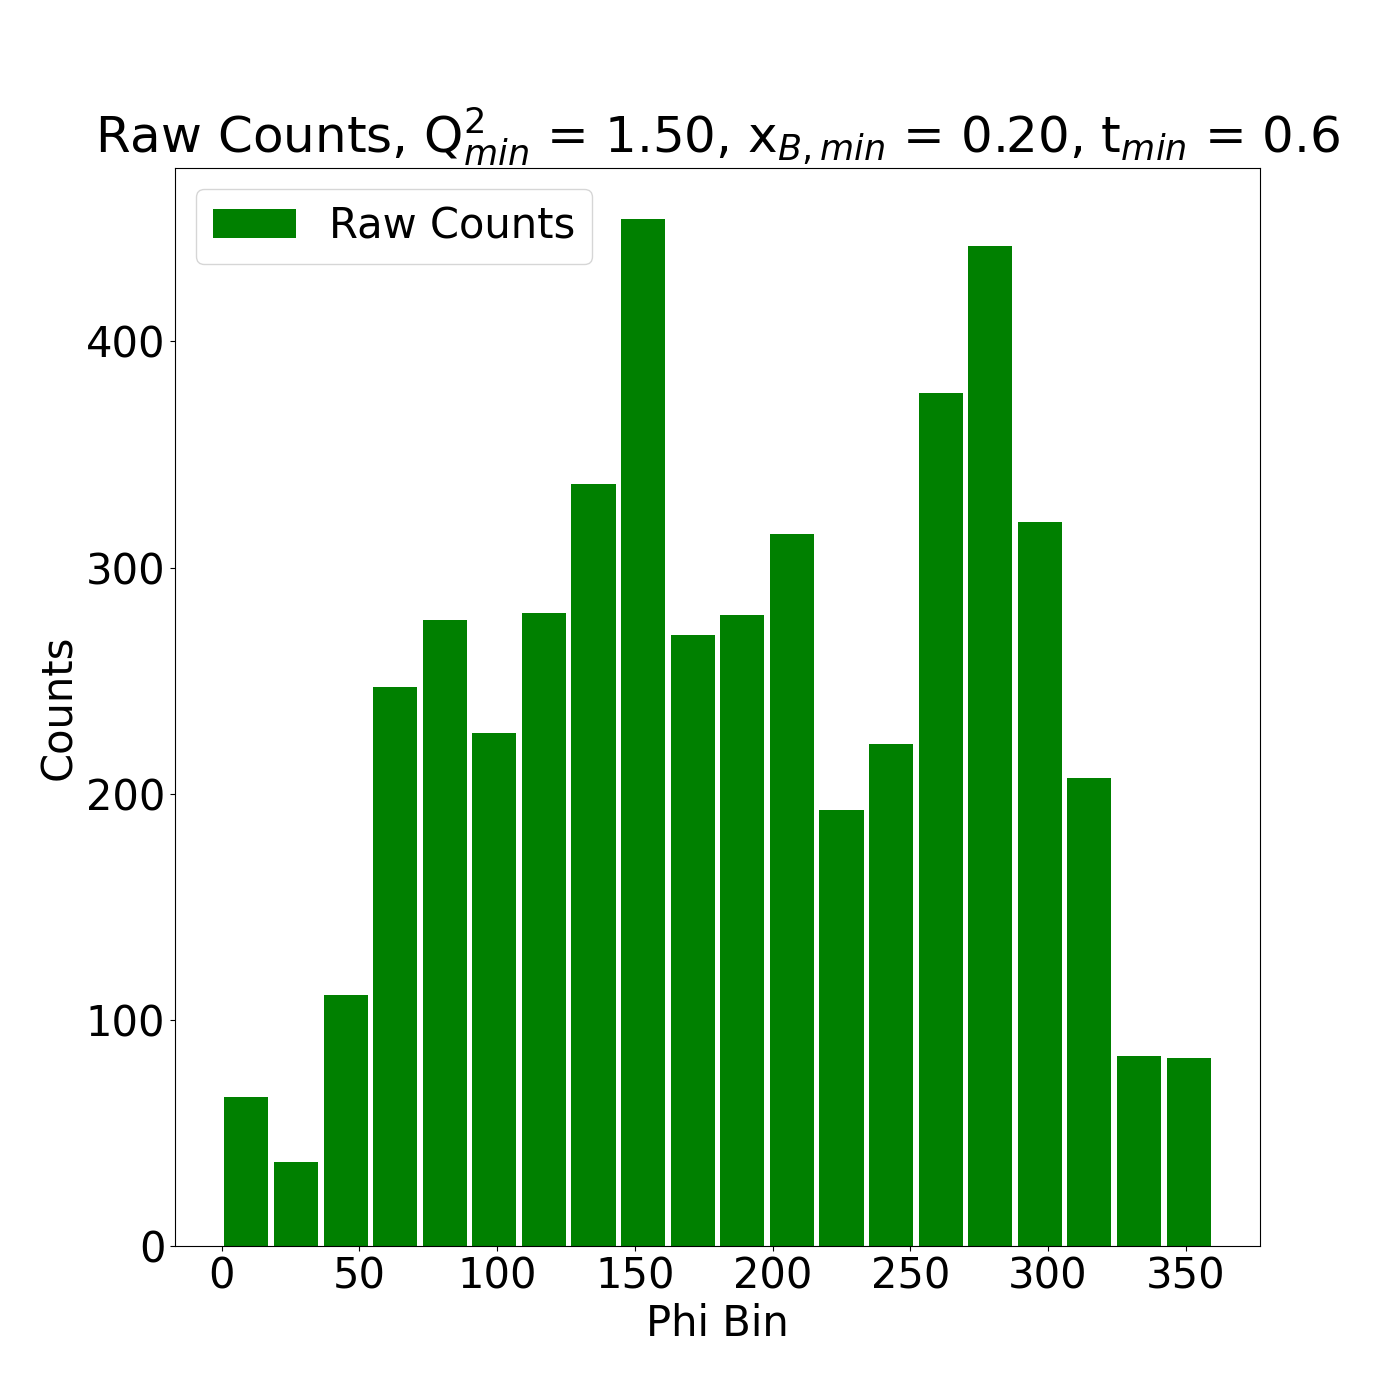
\includegraphics[trim={0 0  0 0cm} ,clip,width=.8982\textwidth]{extra/corrs/raw2.png}


                   	
                	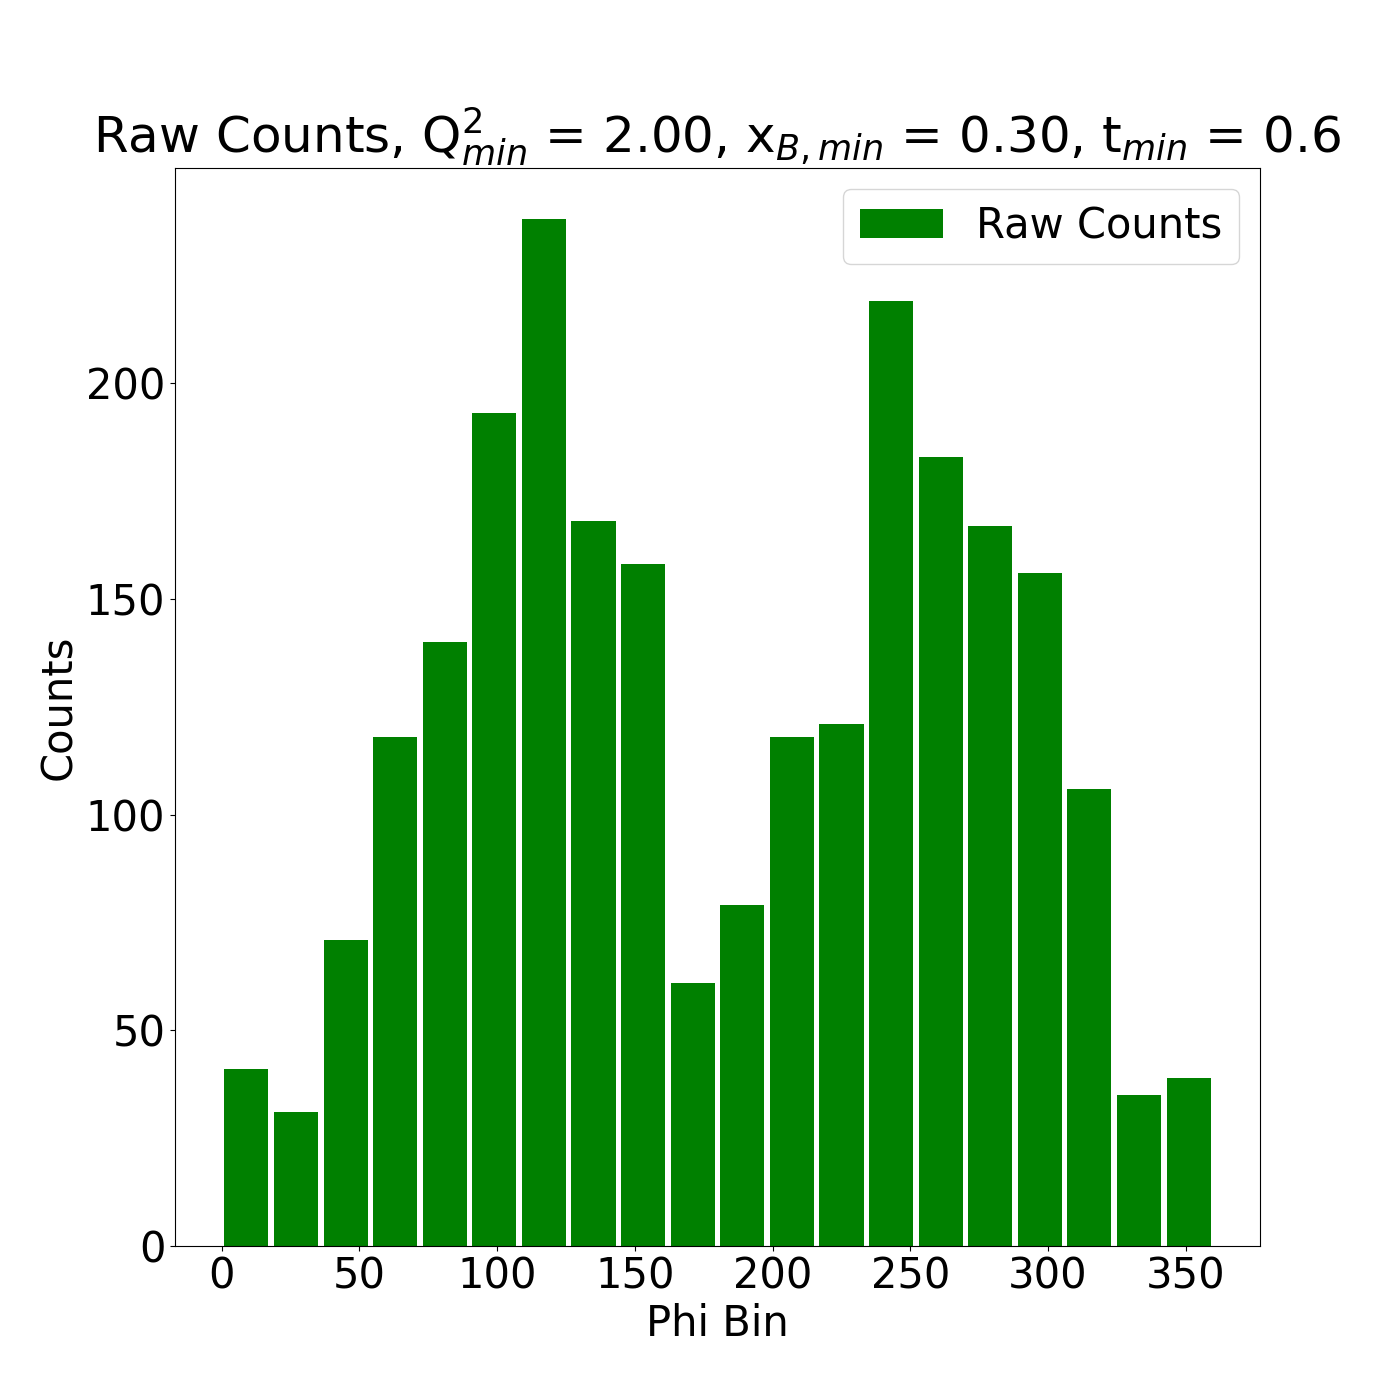
\includegraphics[trim={0 0  0 0cm} ,clip,width=.8982\textwidth]{extra/corrs/raw4.png}


                \column{0.25\textwidth}
     
                       \centering  Simulated $N_{Gen}$, $N_{Rec}$ \\
                	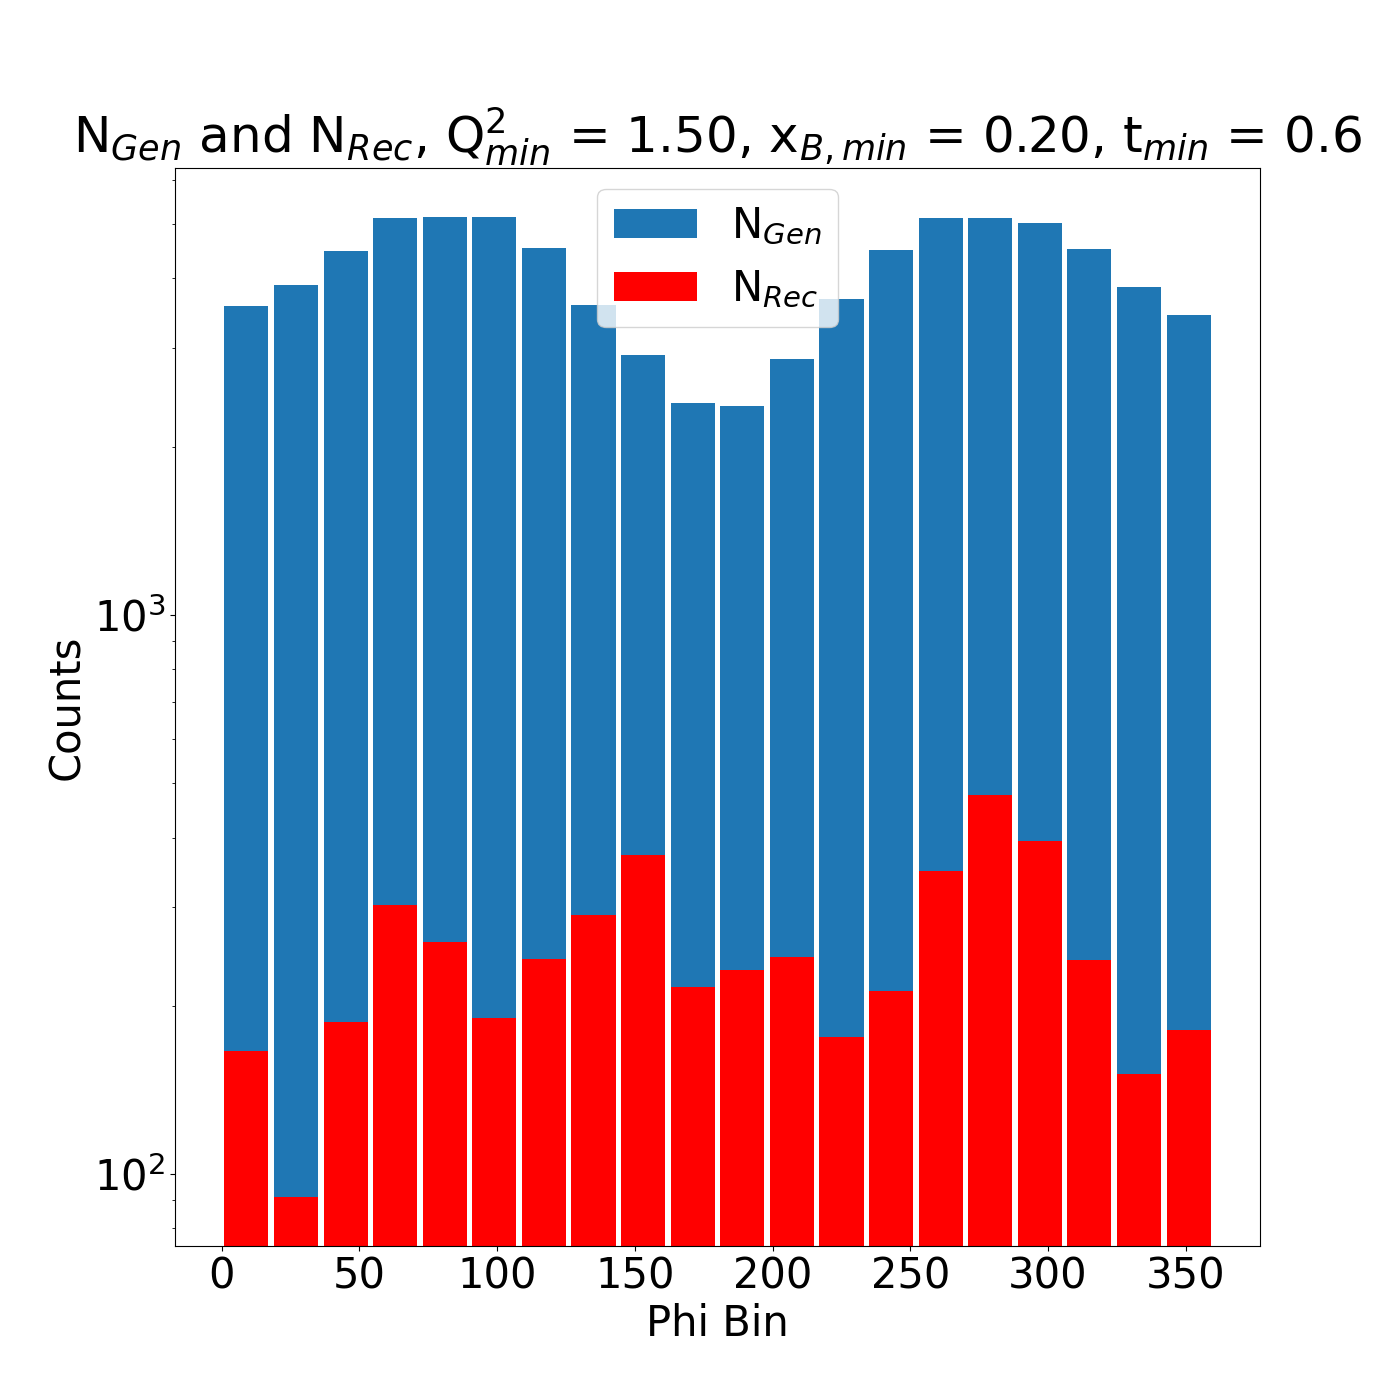
\includegraphics[trim={0 0  0 0cm} ,clip,width=.8982\textwidth]{extra/corrs/acc2.png}
   
                    
                	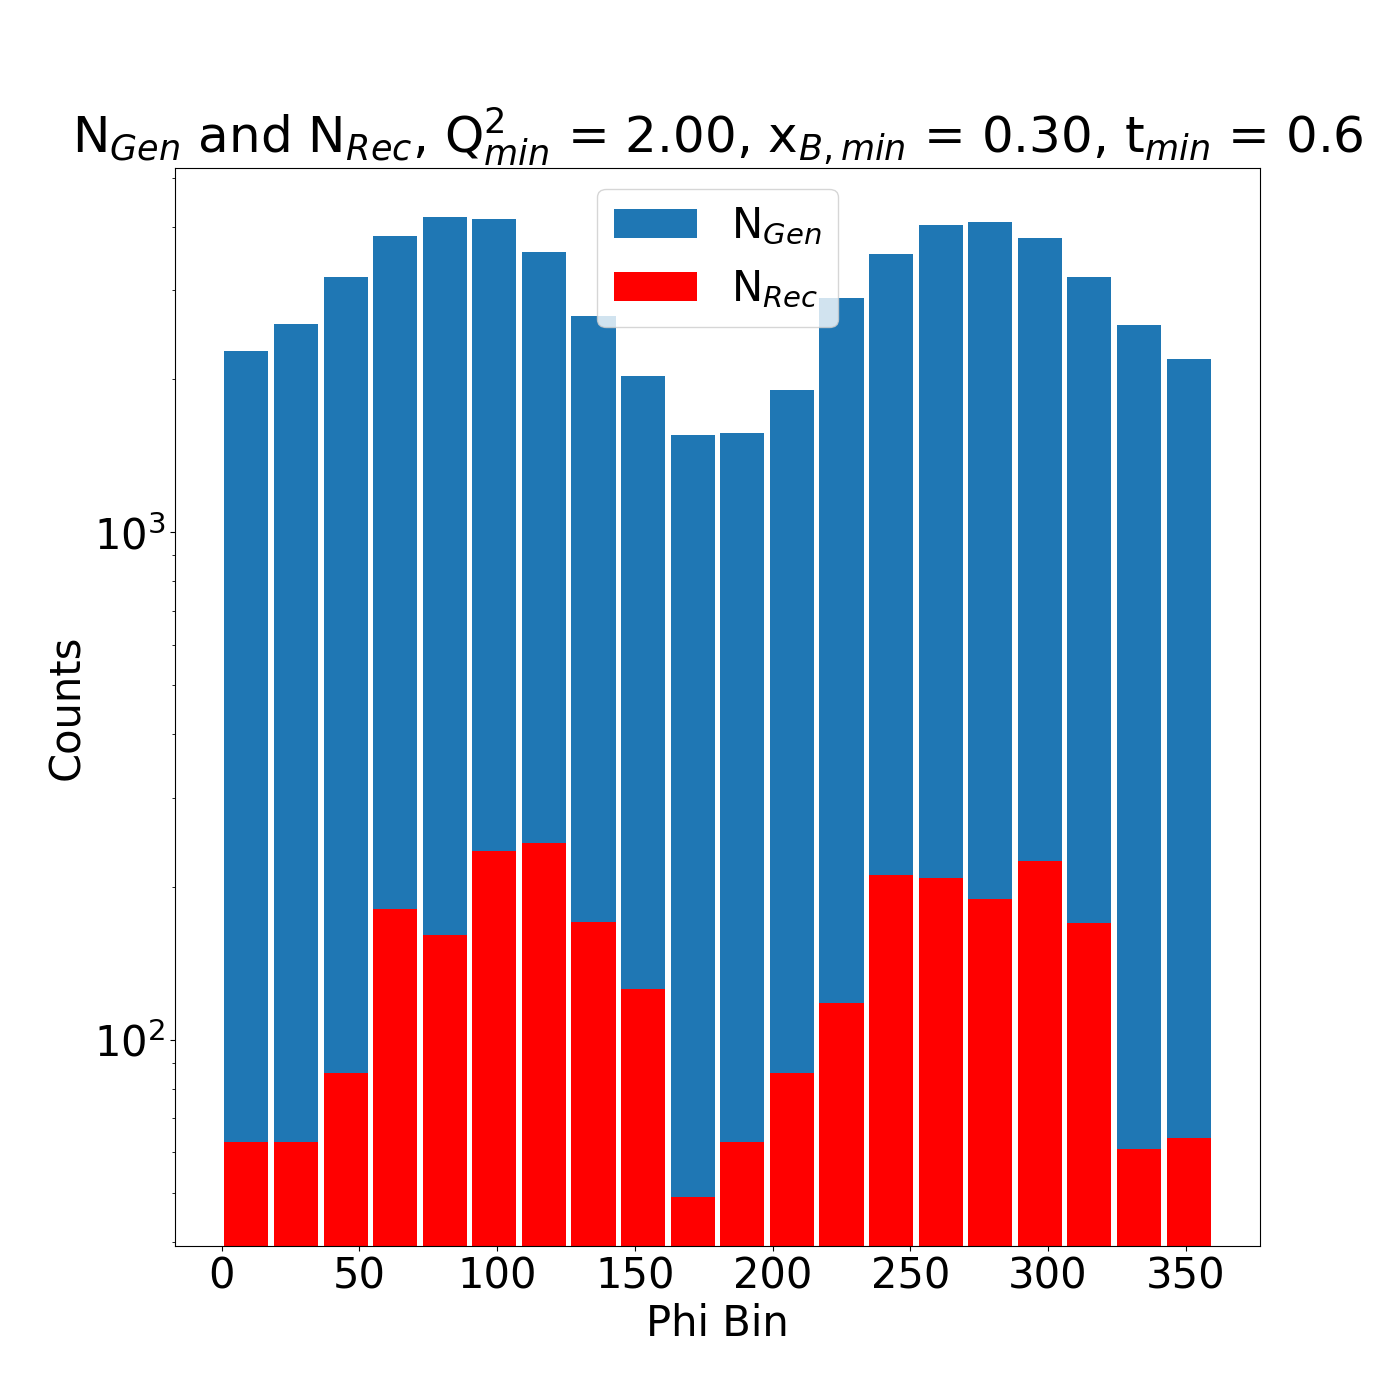
\includegraphics[trim={0 0  0 0cm} ,clip,width=.8982\textwidth]{extra/corrs/acc4.png}

            
            \column{0.25\textwidth}

                    %#---------------------------------------------
                      \centering   Acc. Correction \\
                	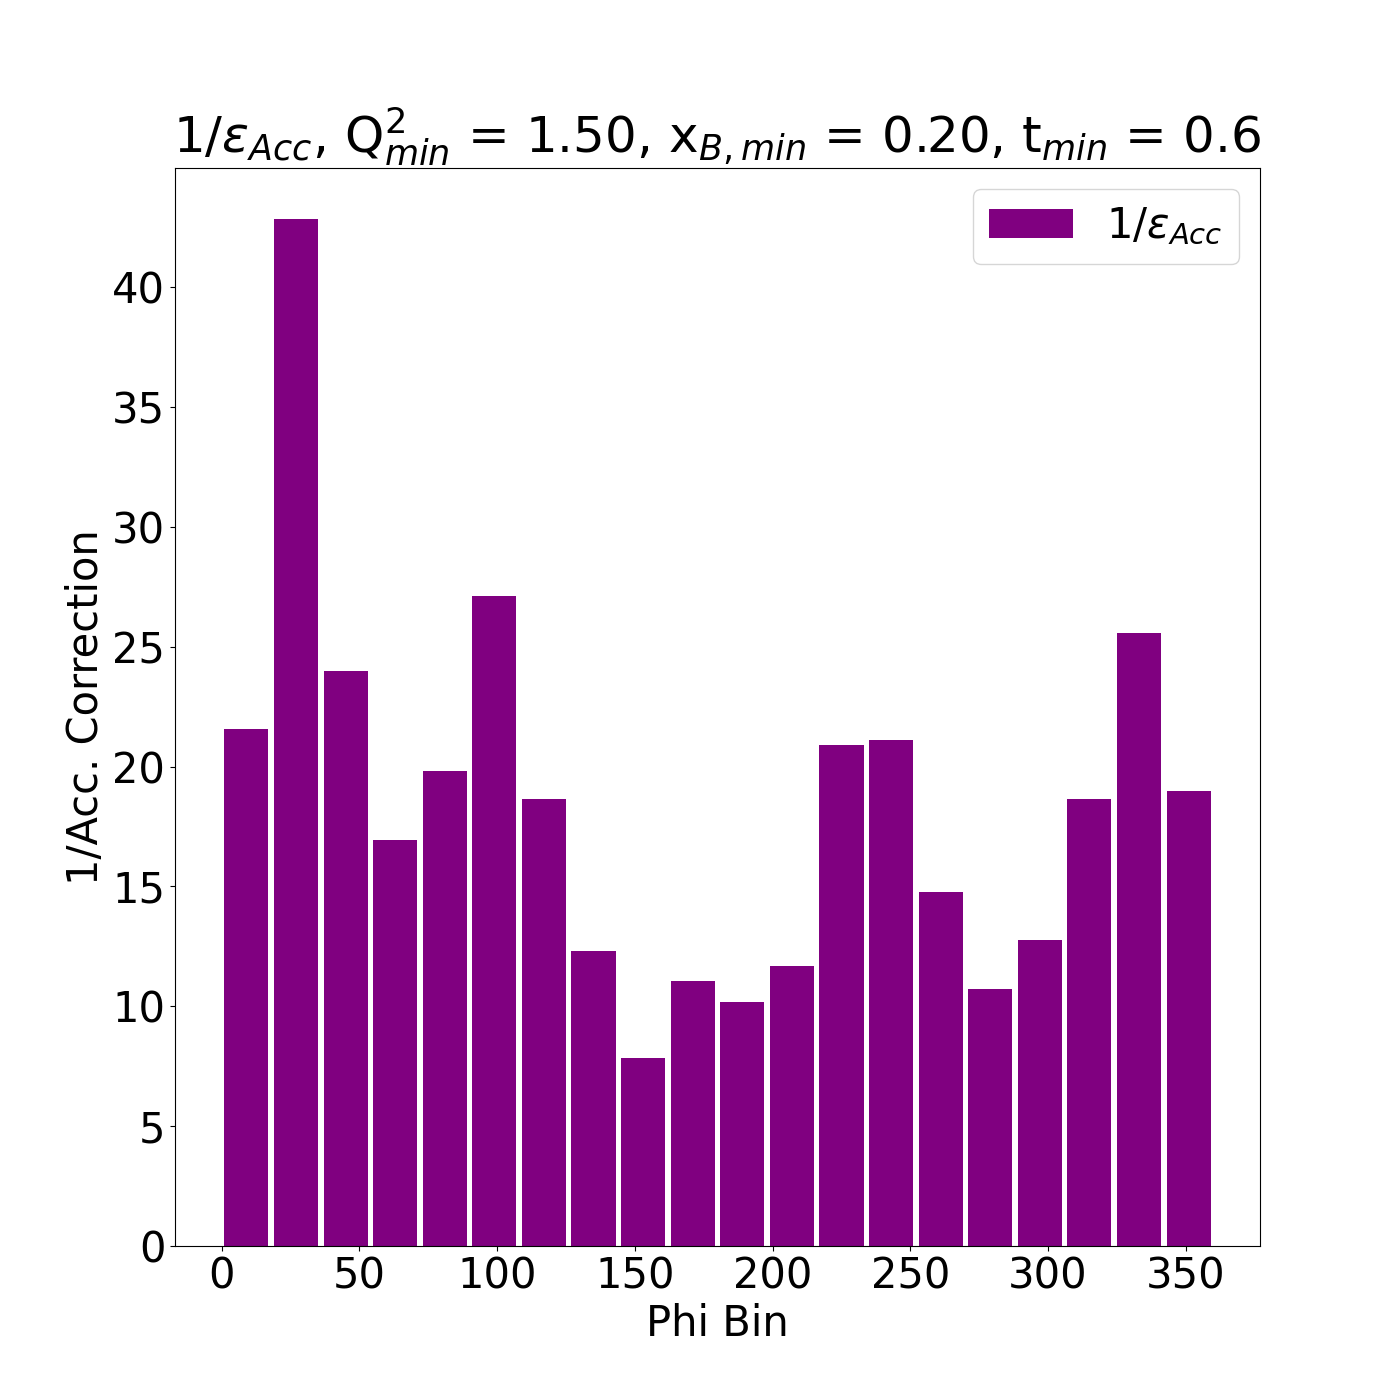
\includegraphics[trim={0 0  0 0cm} ,clip,width=.8982\textwidth]{extra/corrs/raw2acc.png}
 
             
                	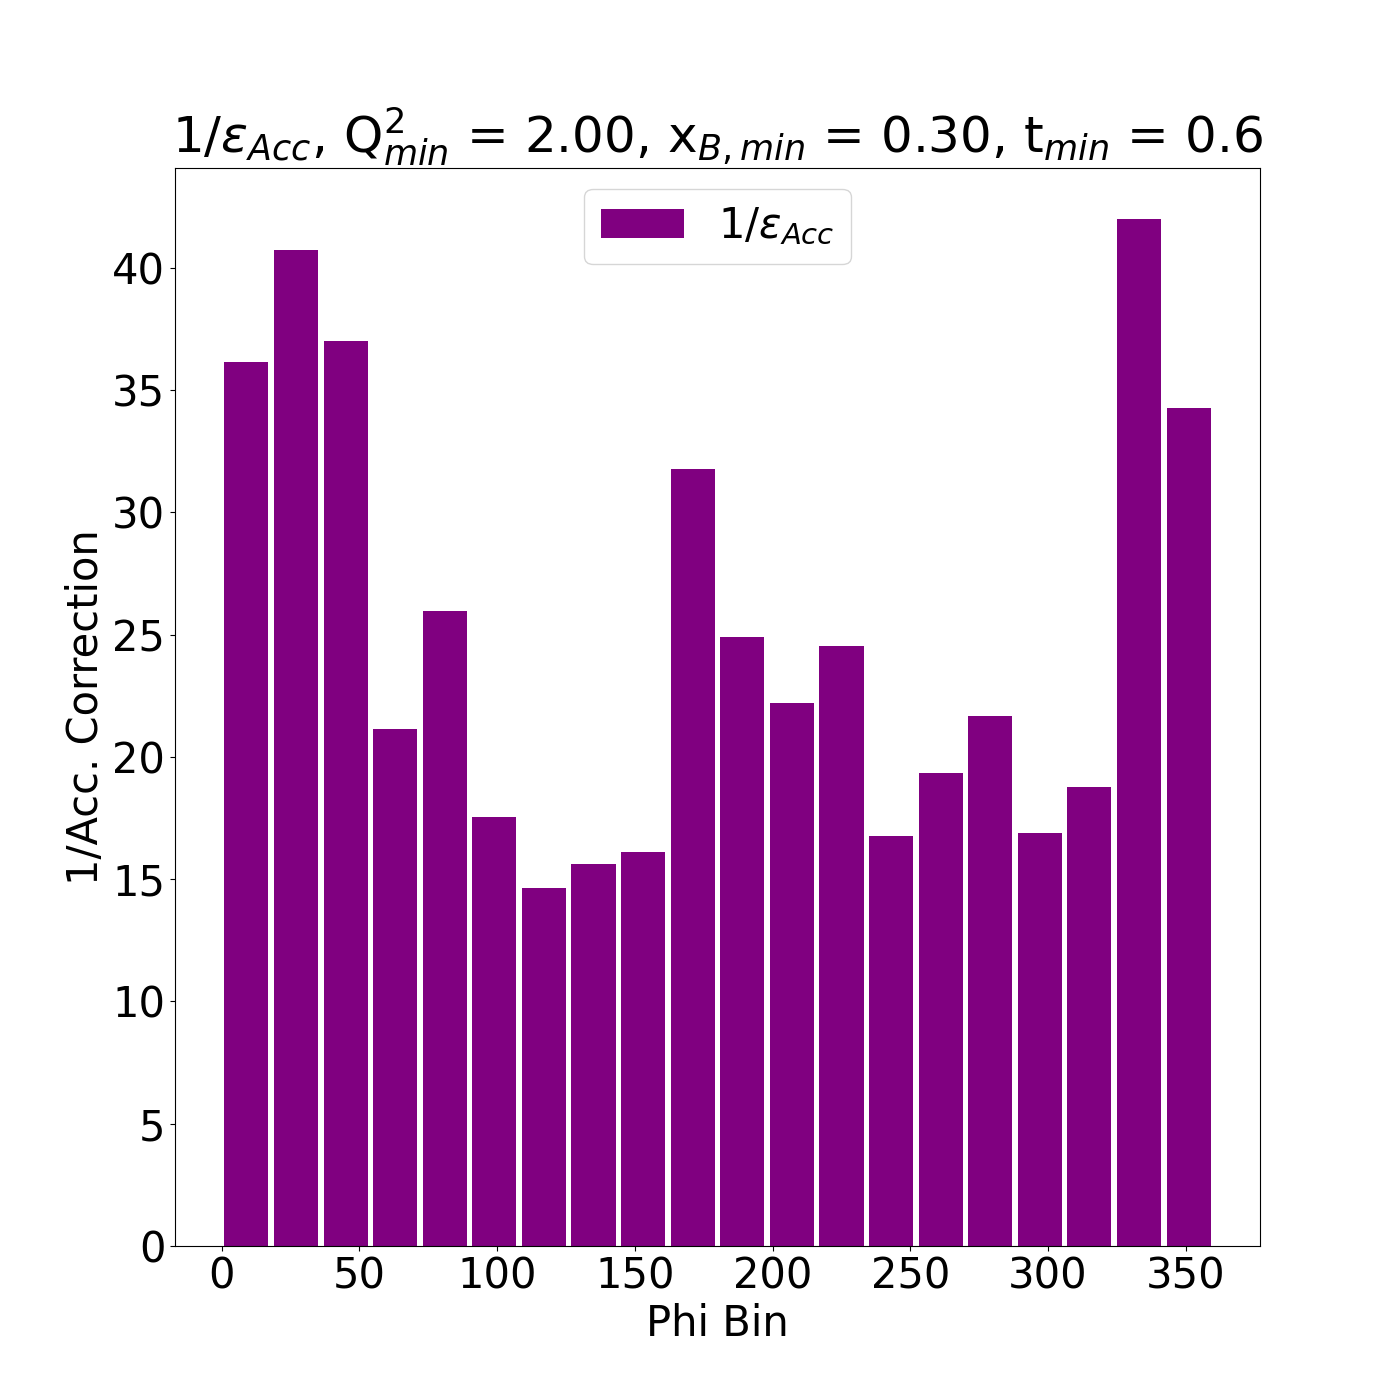
\includegraphics[trim={0 0  0 0cm} ,clip,width=.8982\textwidth]{extra/corrs/acc_3.png}
                	
                	
            \column{0.25\textwidth}

                    %#---------------------------------------------
                      \centering   Acc. Corr. Counts \\
                	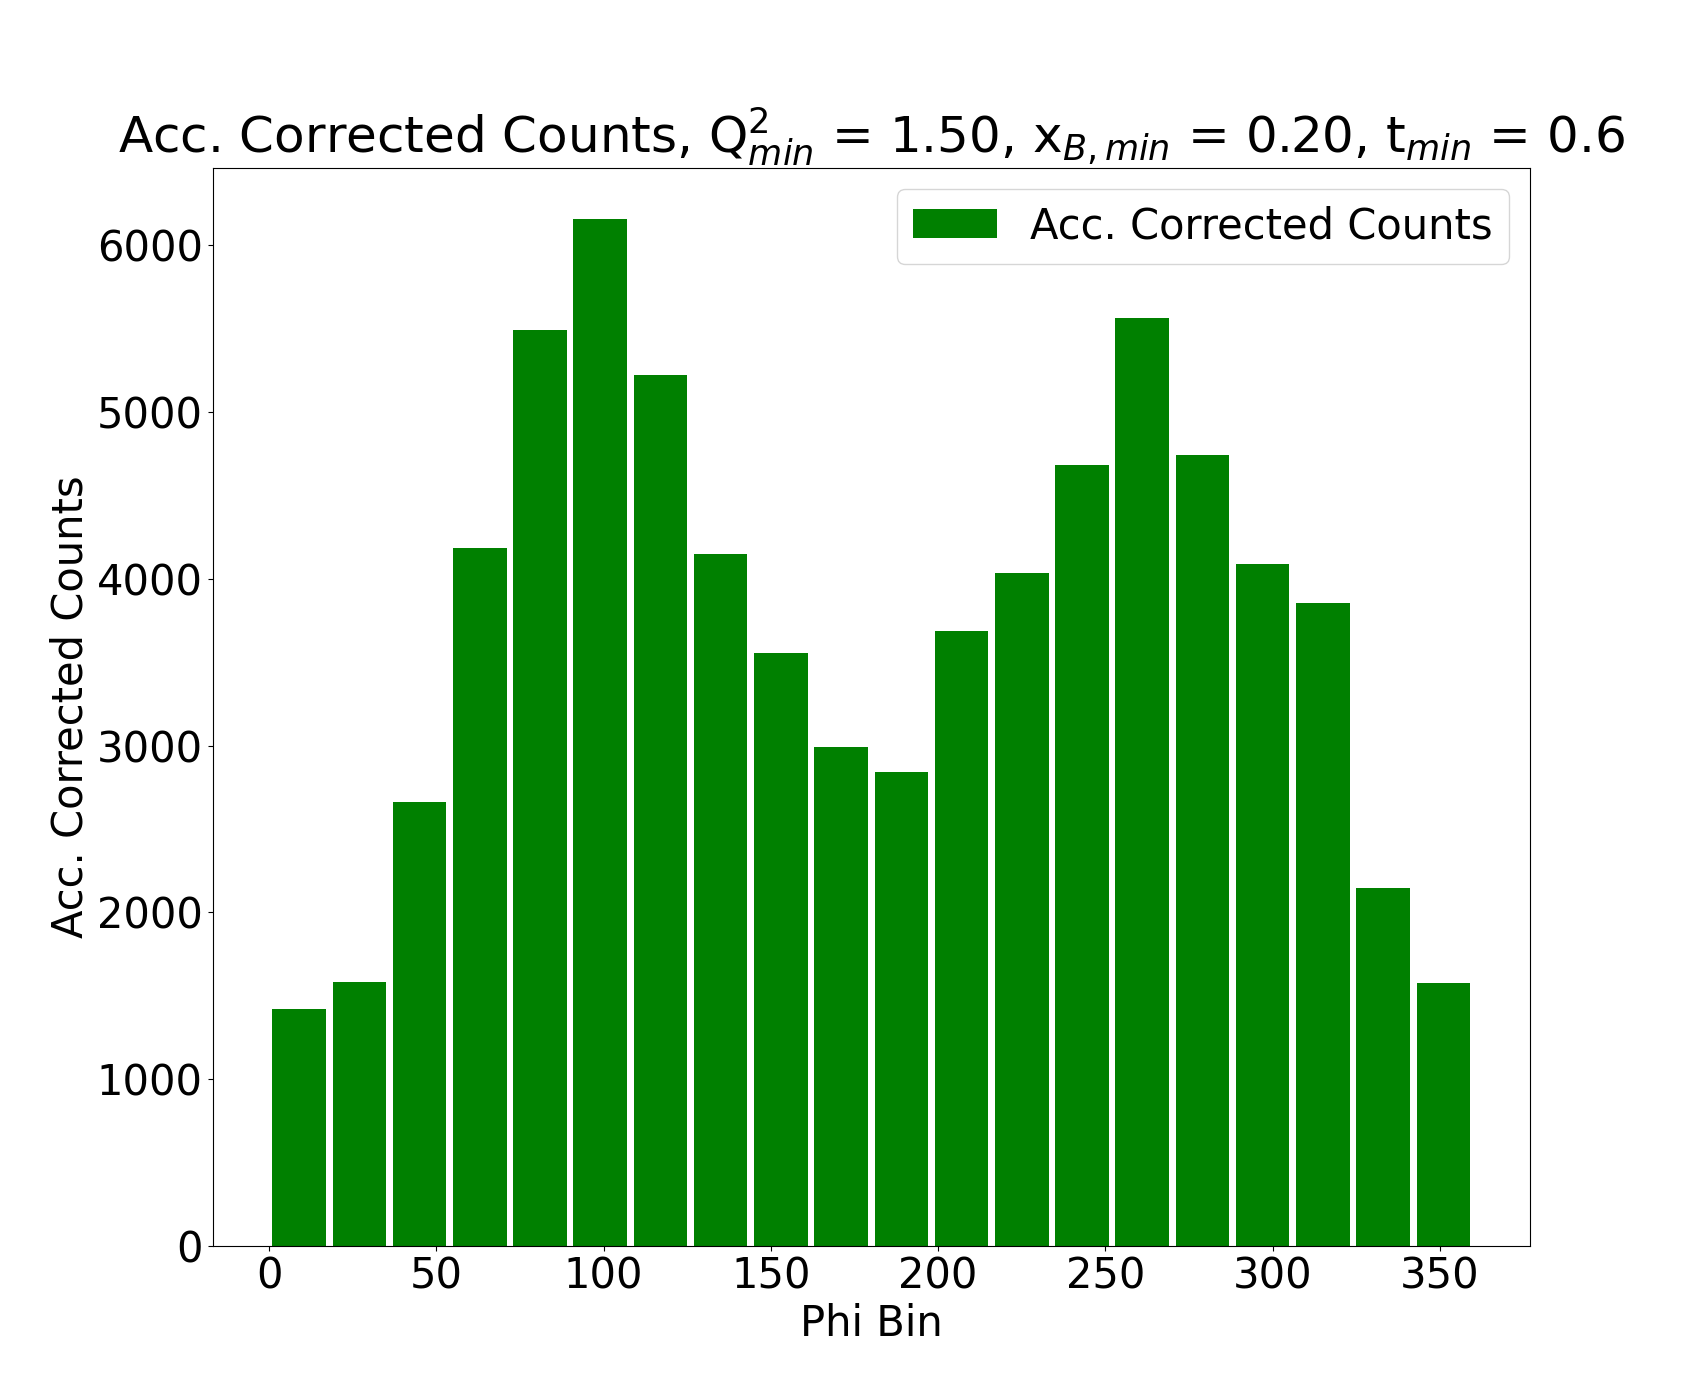
\includegraphics[trim={0 0  0 0cm} ,clip,width=.982\textwidth]{extra/corrs/final1.png}
 
       
                	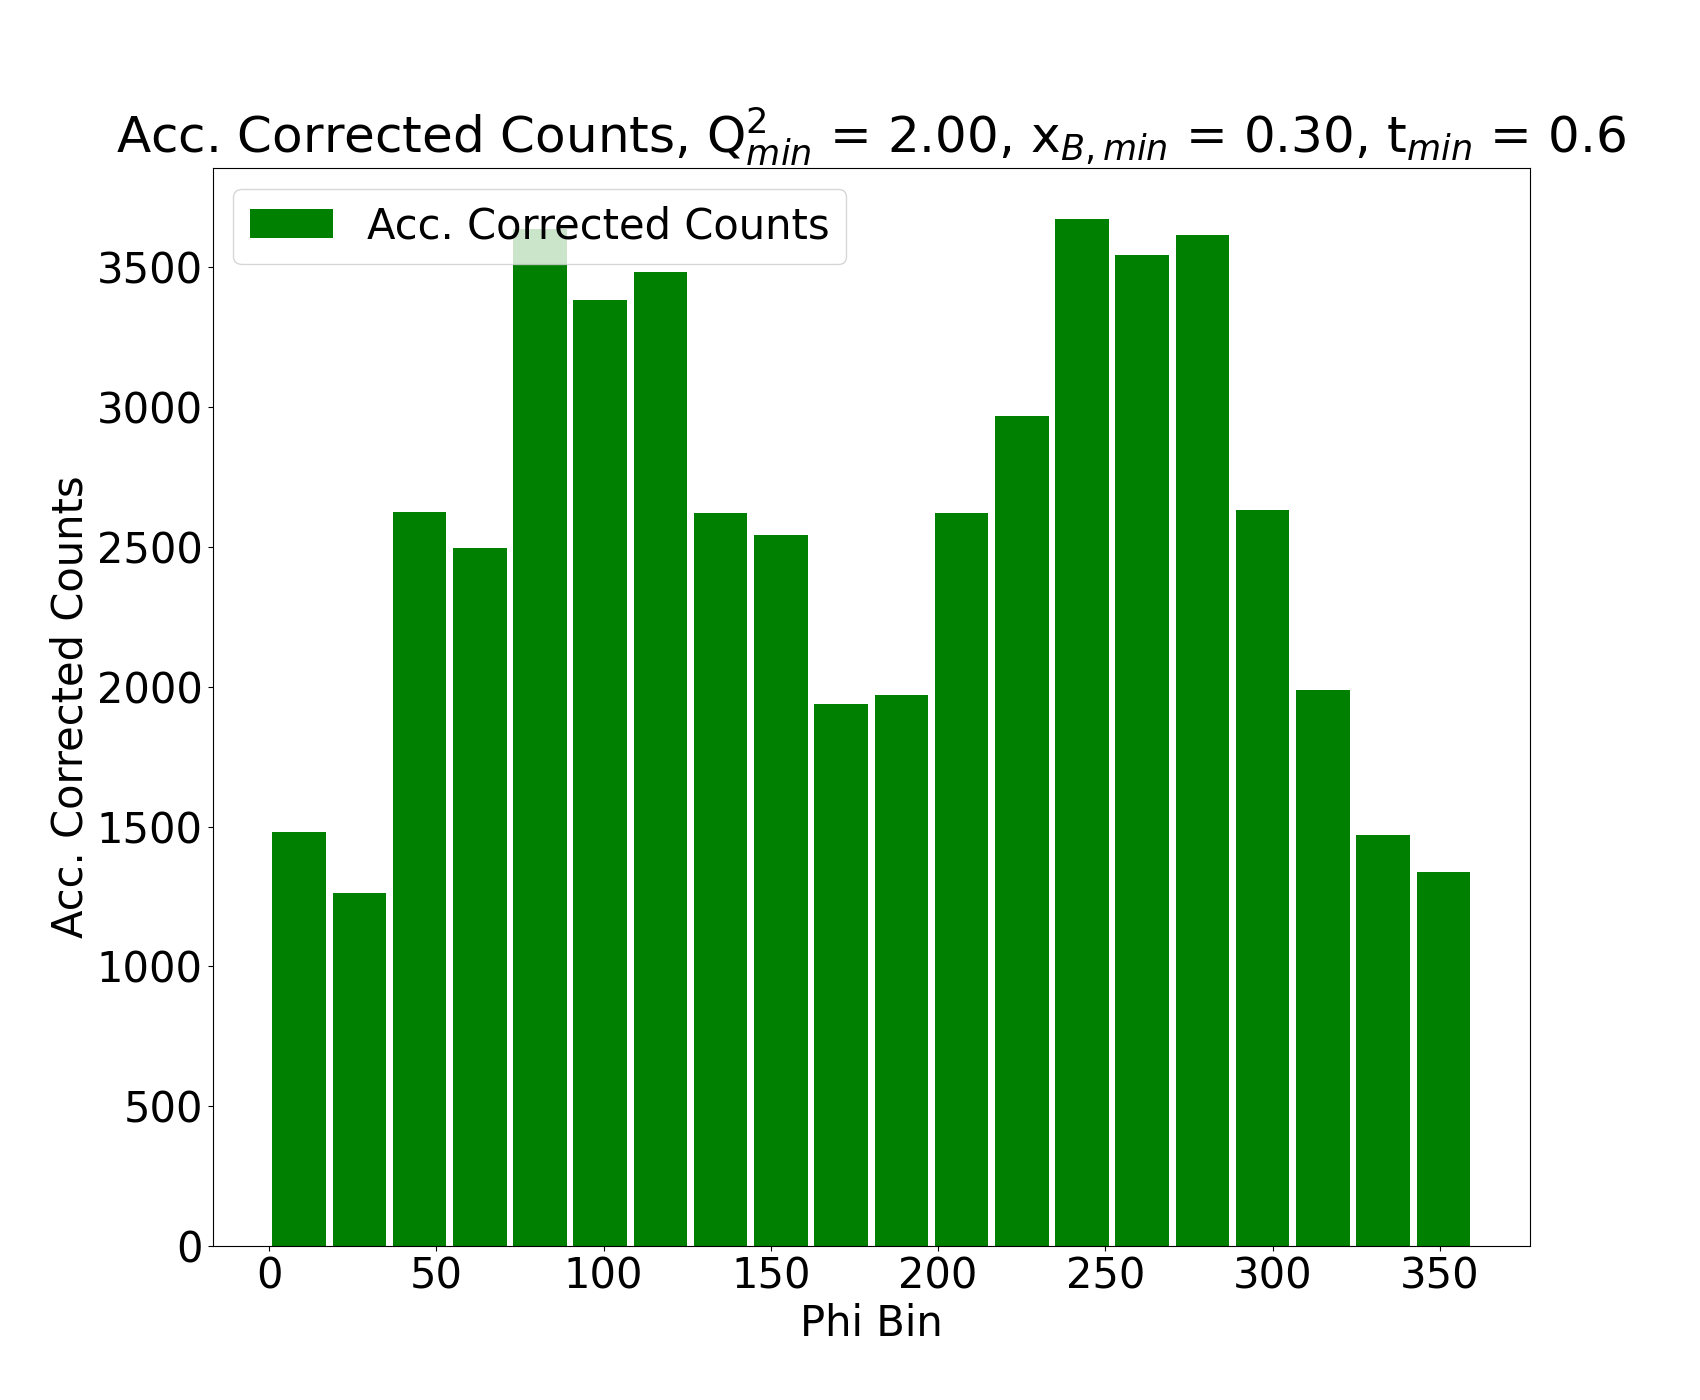
\includegraphics[trim={0 0  0 0cm} ,clip,width=.982\textwidth]{extra/corrs/final2.png}

    \end{columns}
\end{frame}

\begin{frame}{Backup slides}

   \begin{columns}
            \column{0.5\textwidth}
            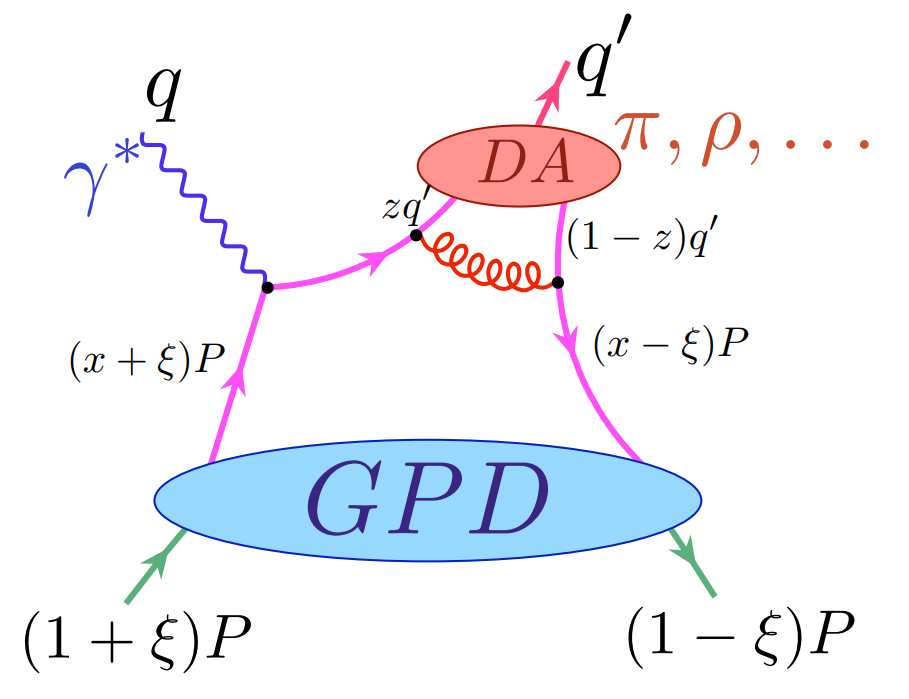
\includegraphics[scale=0.2]{Pics/currentWork/dvpipdiagram.png}\\
            DVMP is sensitive to chiral odd GPDs, distinguishing it from DVCS as a GDP probe\\
            
             \column{0.5\textwidth}
            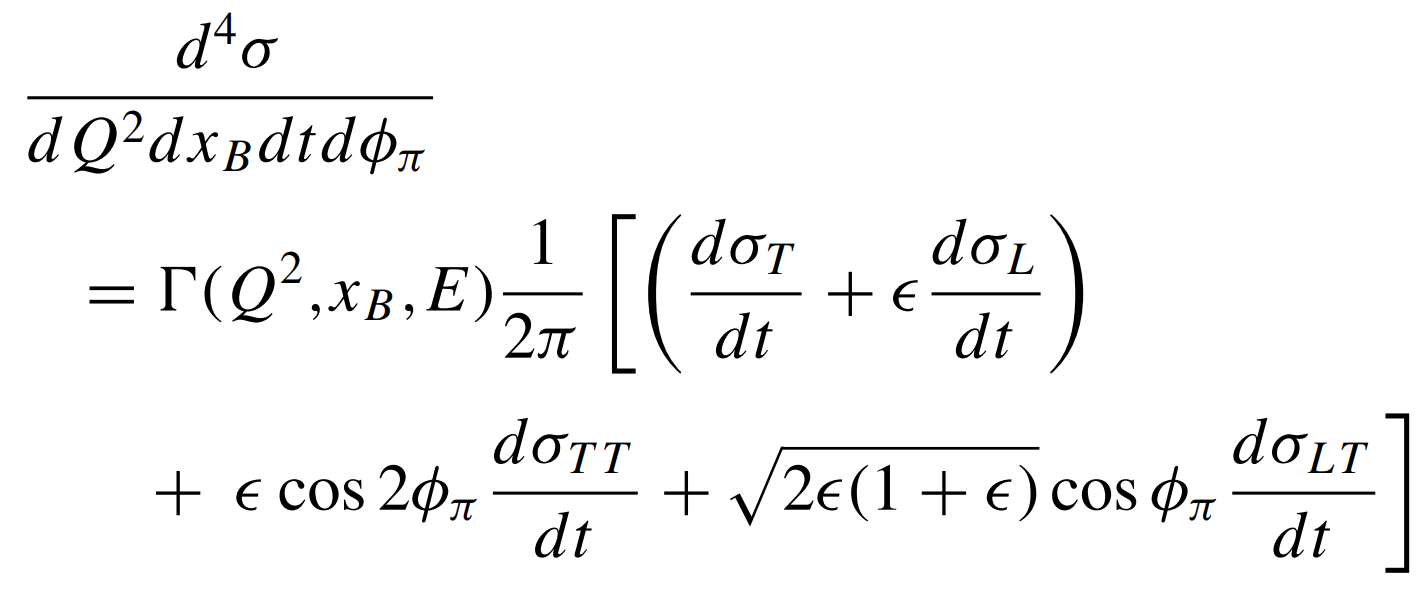
\includegraphics[scale=0.14]{Pics/currentWork/cross-section-formula.png}\\
            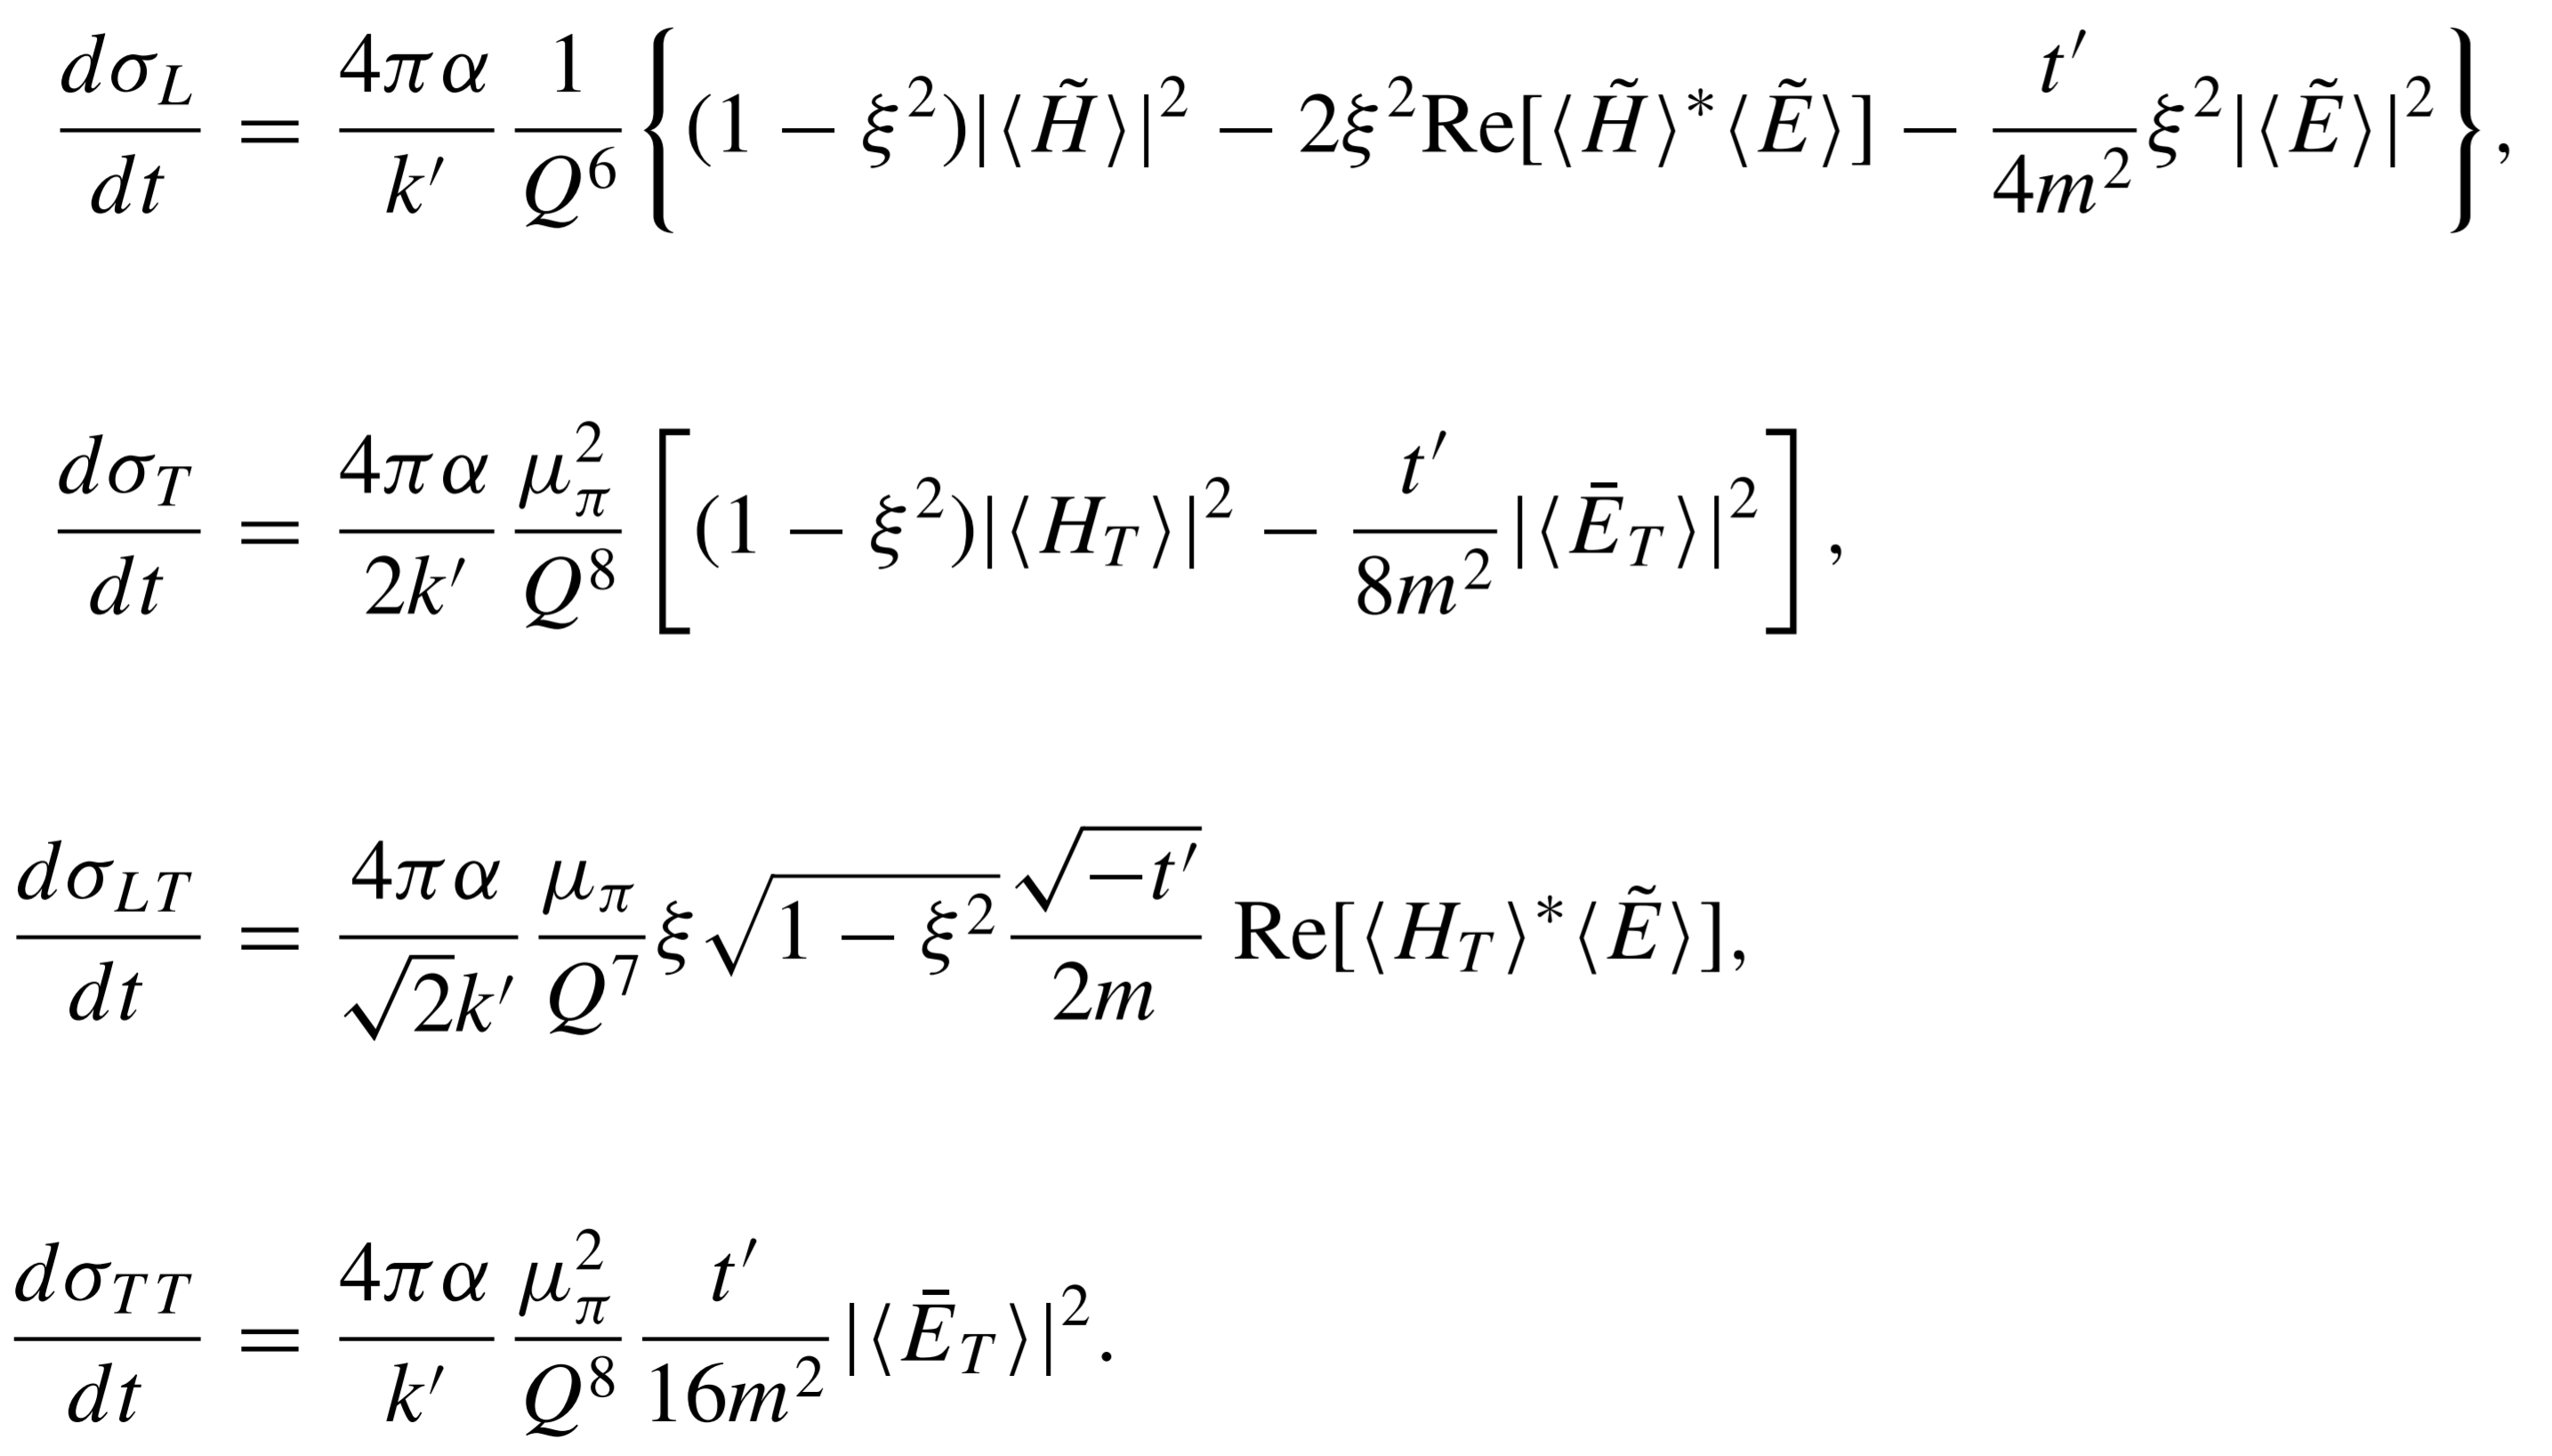
\includegraphics[scale=0.085]{Pics/currentWork/gpds.png}\\
            
    \end{columns}
    
\end{frame}

\begin{frame}{Backup slides}
\centering
Comparision with CLAS6\\

    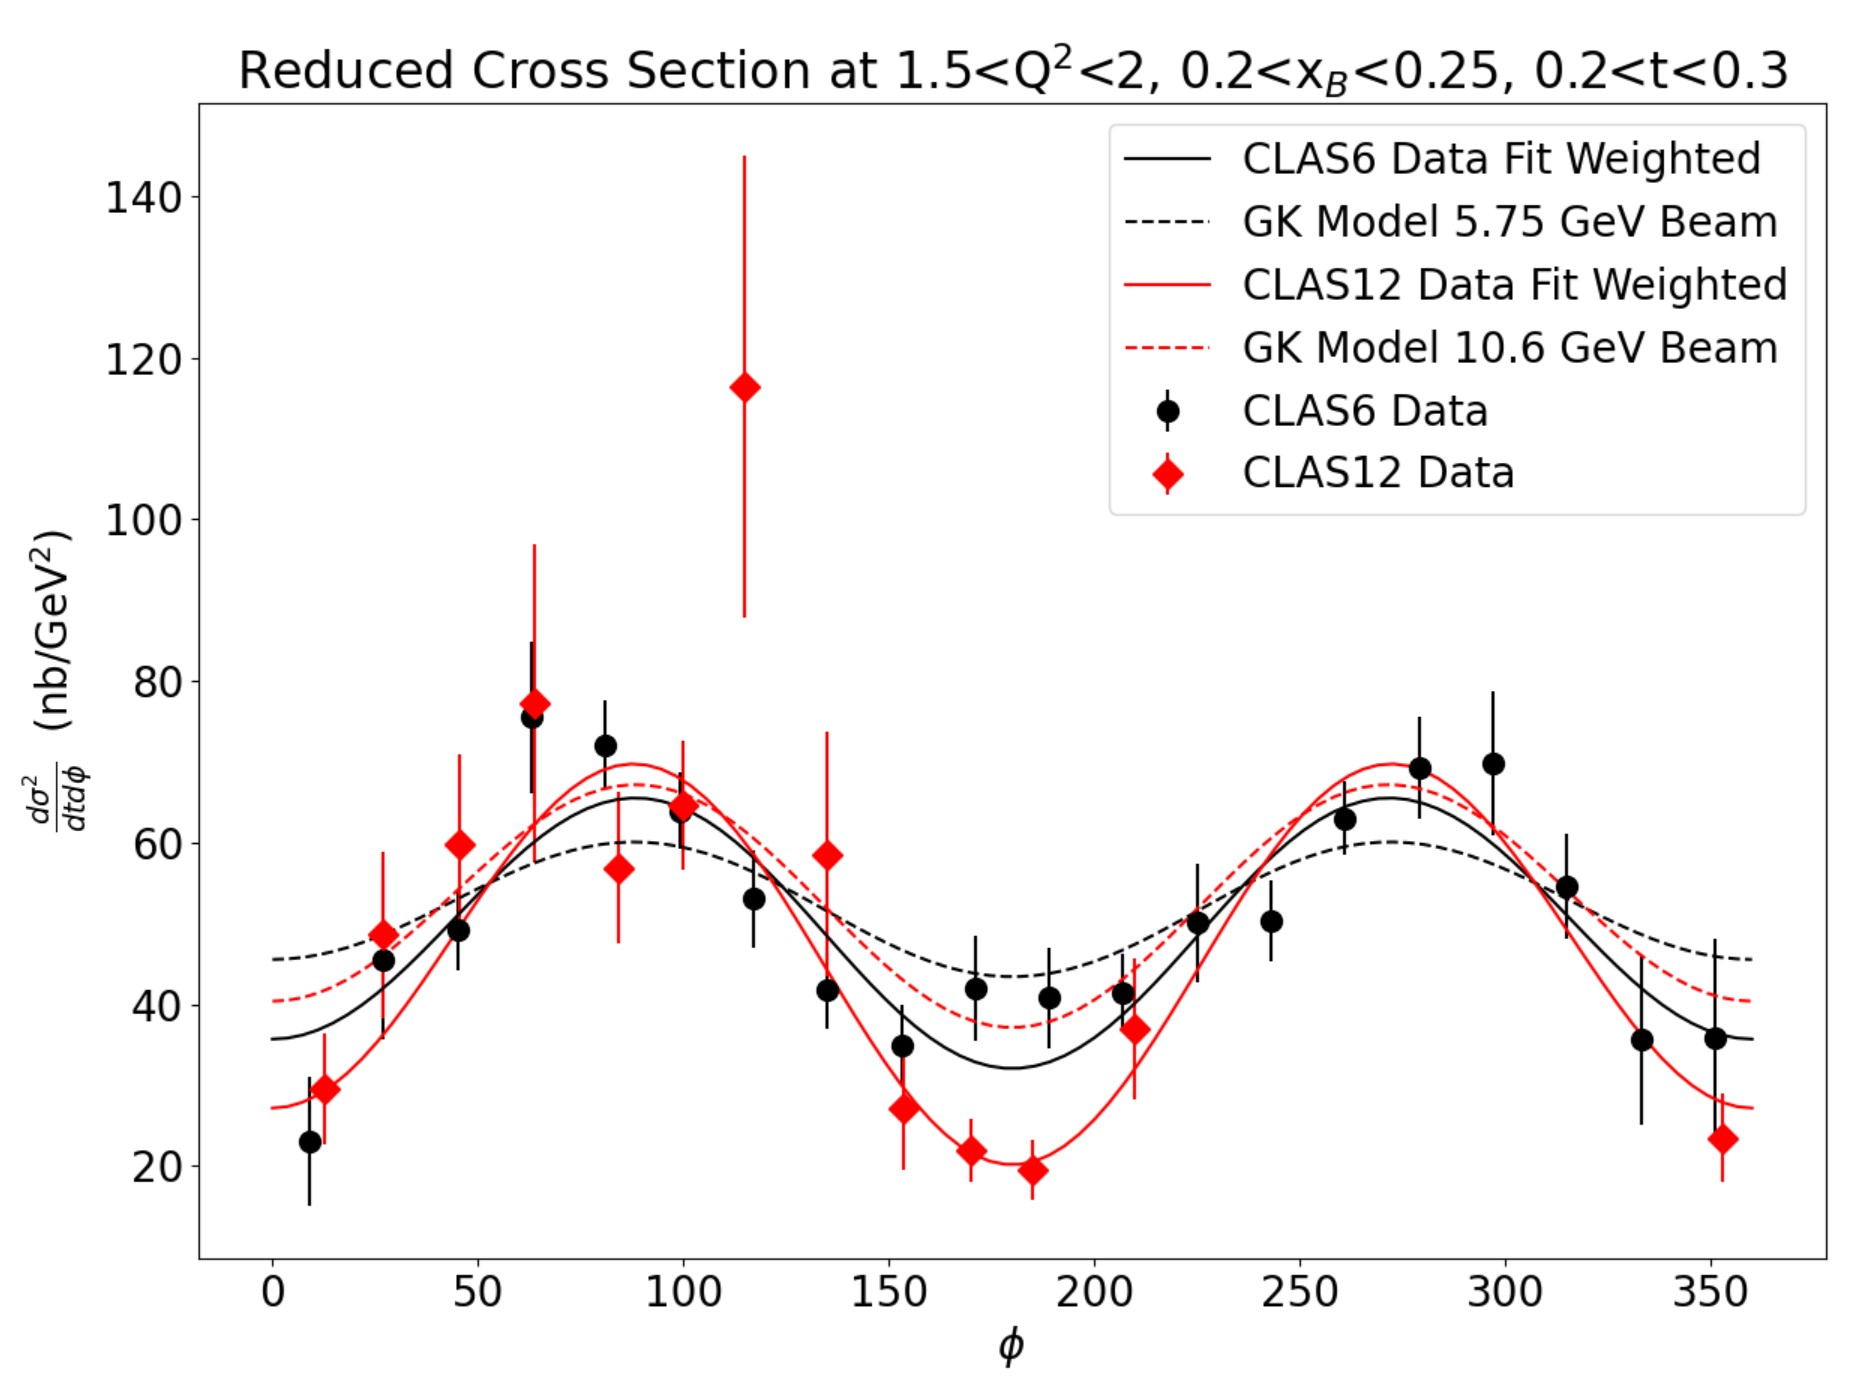
\includegraphics[scale=0.2832]{DNP/comp_c12_gk_c6.jpg}\\
\end{frame}

\begin{frame}{Backup slides}
\centering
Low Q2\\

    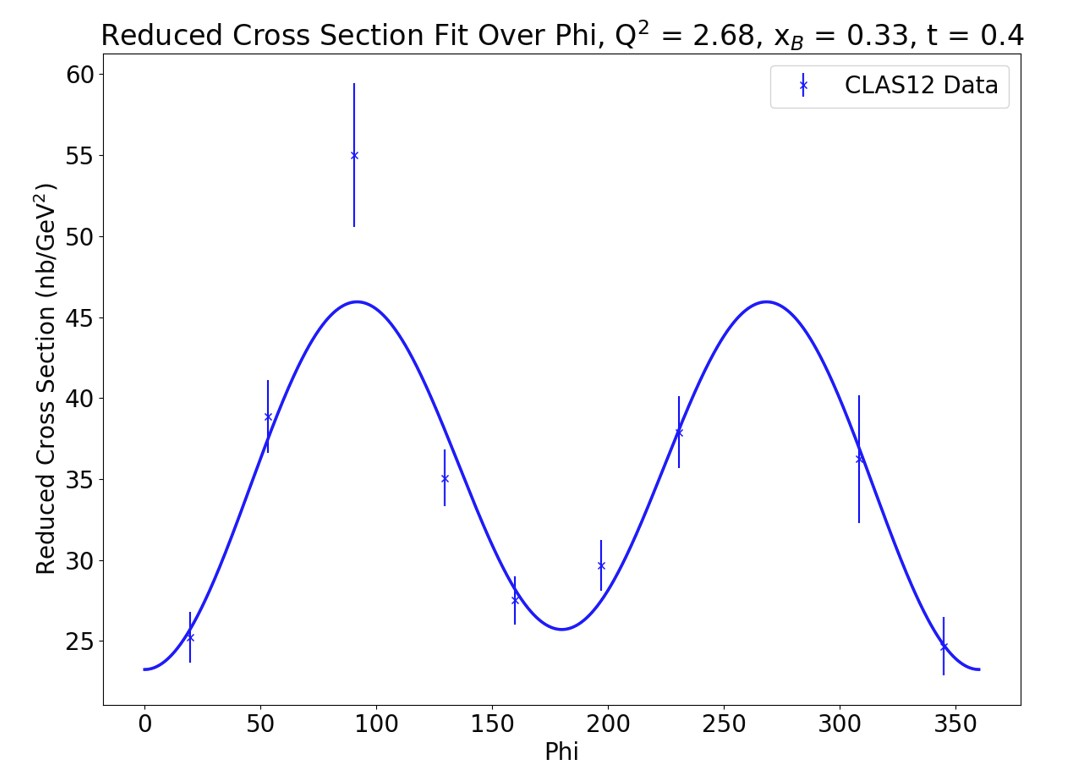
\includegraphics[scale=0.2832]{DNP/beauty_2.jpg}\\
\end{frame}

\begin{frame}{Backup slides}
\centering
Inbending

    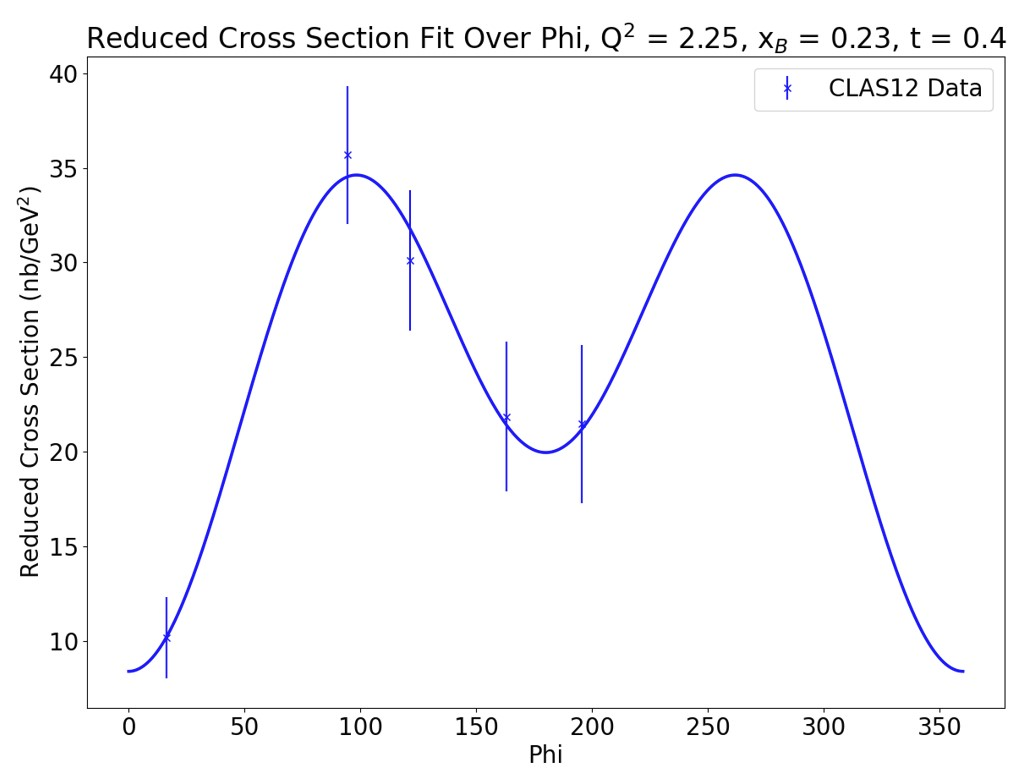
\includegraphics[scale=0.2832]{DNP/nice_inbending.jpg}\\
\end{frame}



\begin{frame}{De-Fence!}
\centering
    

    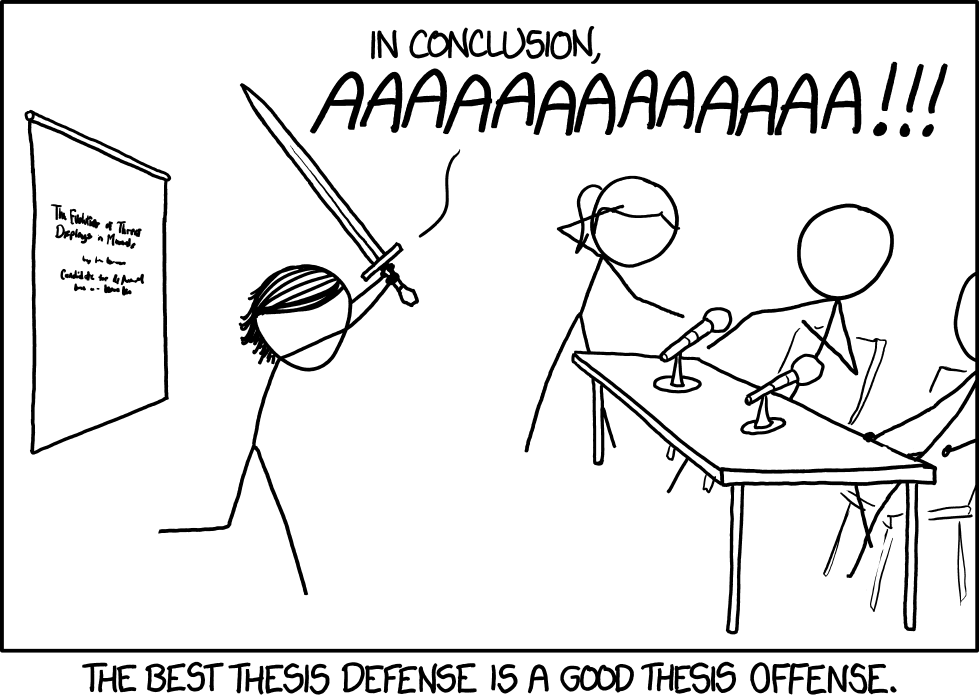
\includegraphics[scale=0.5832]{Main/thesis_defense_2x.png}

    
    {\myfont{\tiny    https://xkcd.com/1403/   }}
\end{frame}




\begin{frame}{Backup slides}
\centering
Other\\

    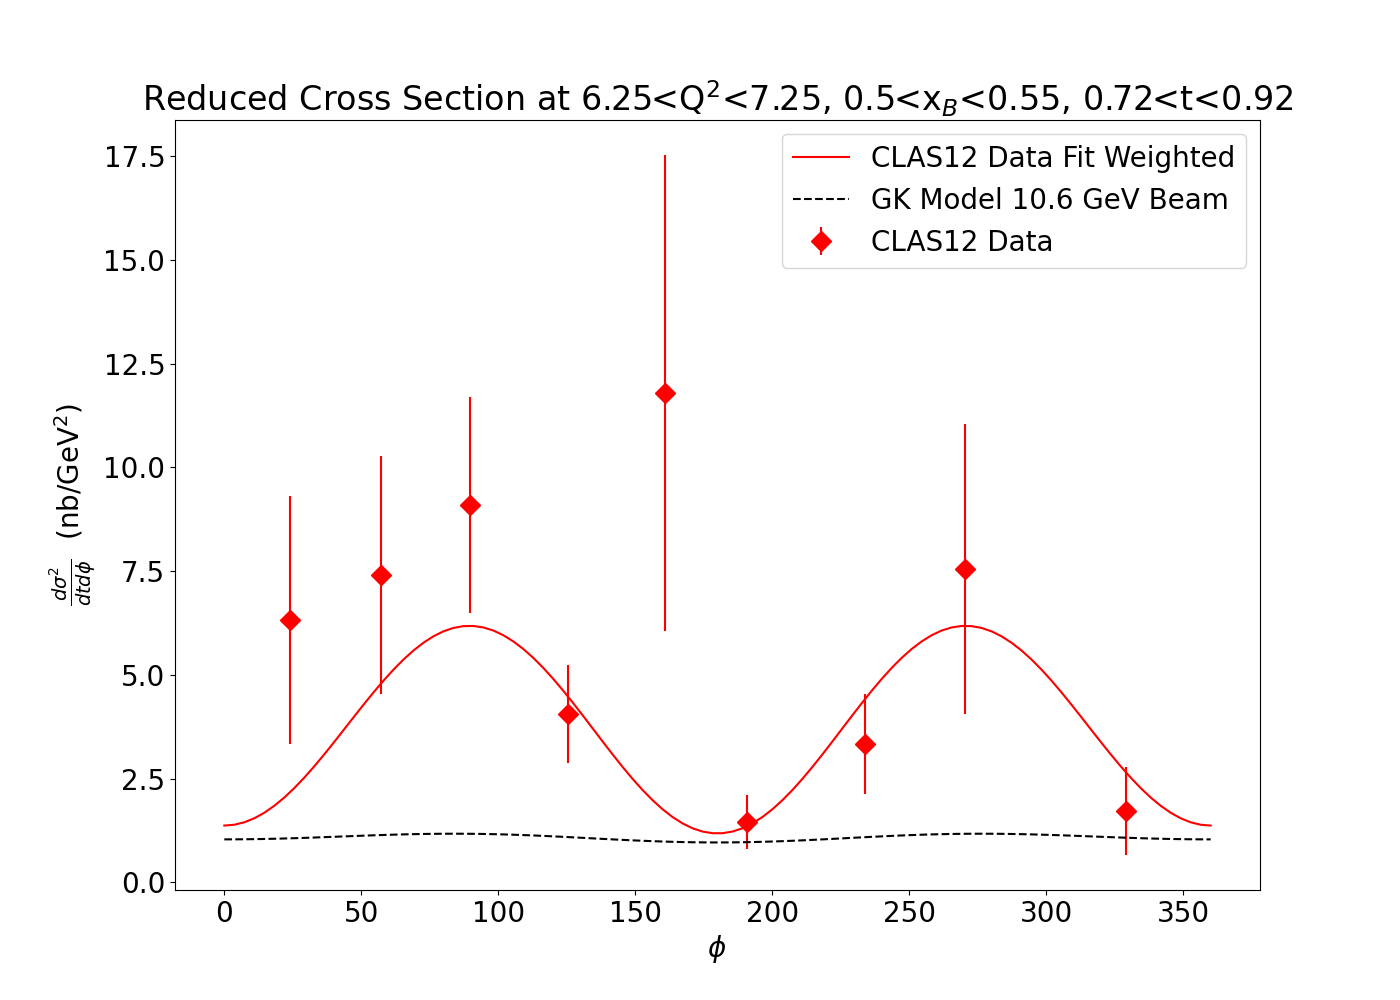
\includegraphics[scale=0.2832]{DNP/finalfig2.png}\\
\end{frame}


\begin{frame}{Backup slides}
\centering
Issues: Misfits\\
    \begin{columns}
             
 
     \column{0.5\textwidth}
    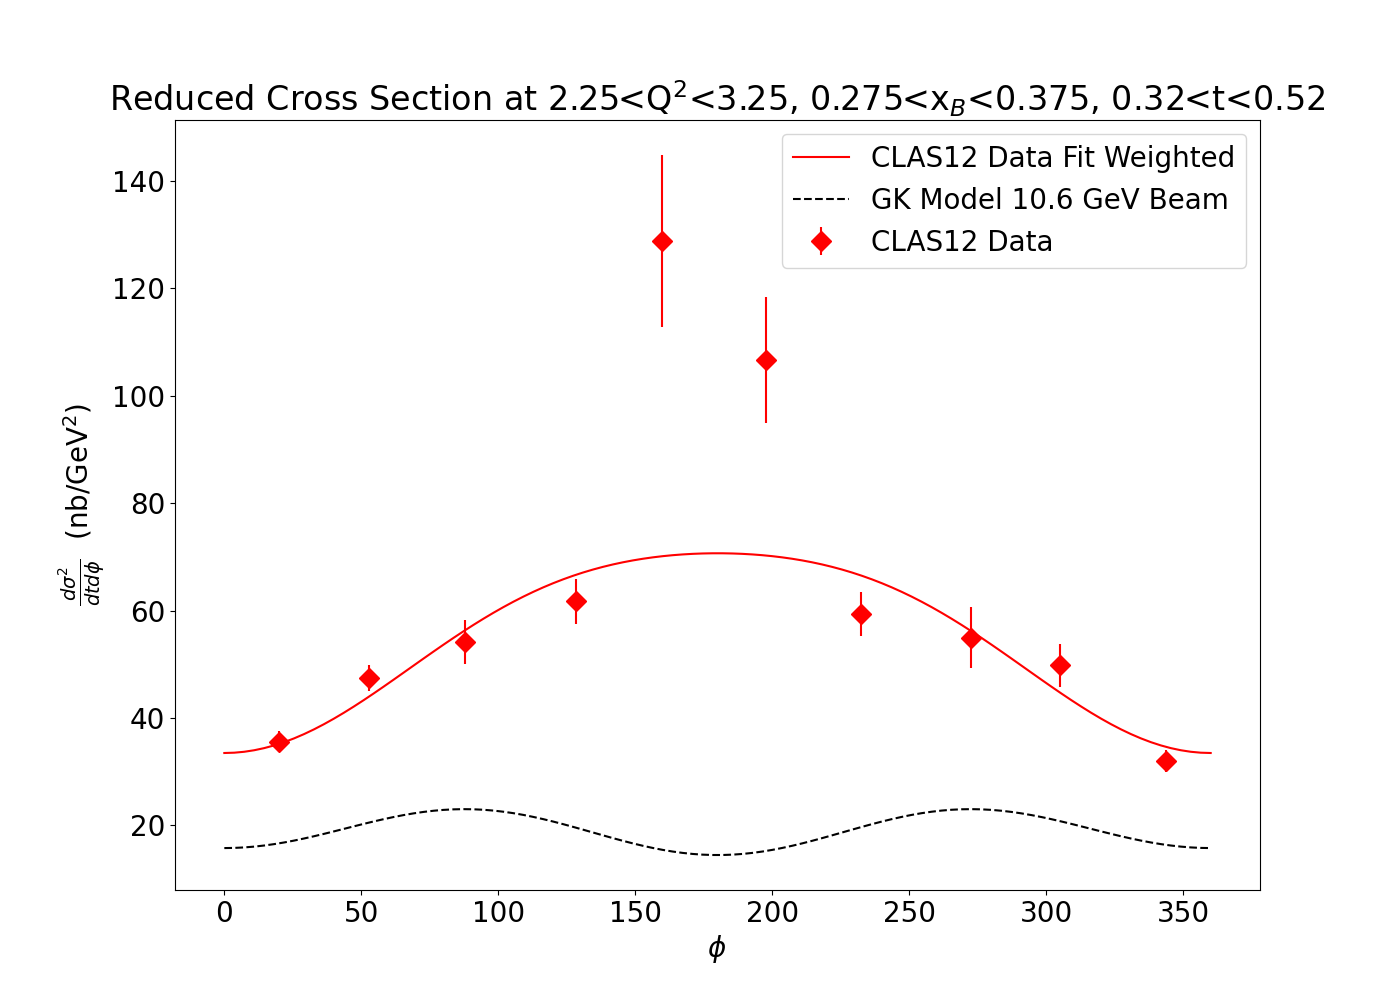
\includegraphics[width=0.95\textwidth]{DNP/misfit_1.png}
     \column{0.5\textwidth}
    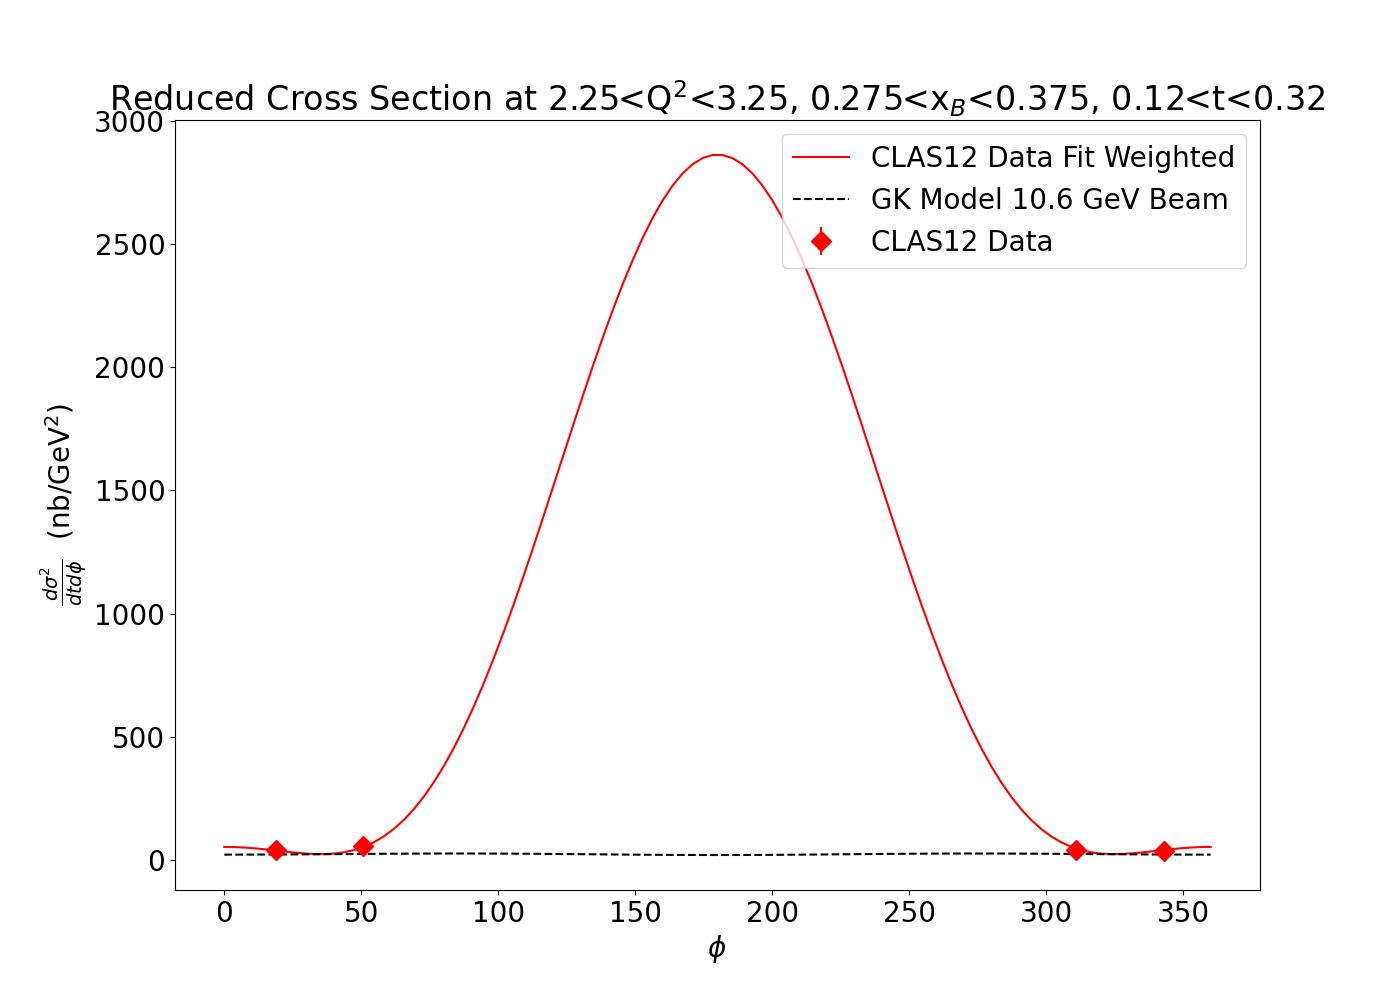
\includegraphics[width=0.95\textwidth]{DNP/misfit_2.png}
       \end{columns}
\end{frame}


\end{document}